\documentclass[11pt,a4paper]{report}

% --- encoding & fonts ---
\usepackage[T1]{fontenc}
\usepackage[utf8]{inputenc}
\usepackage{lmodern}

% --- sane page margins ---
\usepackage[a4paper,margin=2.6cm]{geometry}

% --- typography: this is what fixes the "jumps" ---
\usepackage{microtype}
\usepackage{parskip}
\usepackage{setspace}
\onehalfspacing            % swap to \singlespacing for denser text
\setlength{\emergencystretch}{3em}

% --- figures & tables (array + calc are what make the wide tables render) ---
\usepackage{graphicx}
\usepackage{float}
\usepackage{array}
\usepackage{calc}
\usepackage{longtable}
\usepackage{ltcaption}
\usepackage{booktabs}
\usepackage{caption}
\captionsetup{font=small,labelfont=bf}

% --- math, citations, links ---
\usepackage{amsmath,amssymb}
\usepackage[numbers,sort&compress]{natbib}
\usepackage[hidelinks]{hyperref}

% --- Pandoc helpers still referenced by the chapters ---
\providecommand{\tightlist}{\setlength{\itemsep}{0pt}\setlength{\parskip}{0pt}}
\providecommand{\pandocbounded}[1]{#1}

\begin{document}

% ------------------- Title page (Università di Messina) -------------------
\begin{titlepage}
  \centering
  
\includegraphics[width=0.24\textwidth]{unime-logo.jpg}\\[10pt]
  {\Large\textsc{Universit\`a degli Studi di Messina}}\\[4pt]
  \rule{\linewidth}{0.4mm}\\[6pt]
  {\small\bfseries DIPARTIMENTO DI SCIENZE MATEMATICHE E INFORMATICHE,\\
   SCIENZE FISICHE E SCIENZE DELLA TERRA}\\[6pt]
  {\normalsize Master's Degree in Data Science (LM-DATA)}\\
  {\normalsize Curriculum: Economics}\\[26mm]

  {\LARGE\bfseries Scalable Real-Time Hate Speech Detection}\\[8pt]
  {\large A Big Data Architecture utilizing Stream Processing and\\
   Deep Learning with Automated AI Agents}\\[24mm]

  \noindent
  \begin{minipage}[t]{0.5\textwidth}
    \raggedright\large
    \textbf{Supervisor:}\\ Prof.\ Francesco La Rosa\\[8pt]
    \textbf{Co-Supervisor:}\\ Dr.\ Pierluigi Dell'Acqua
  \end{minipage}\hfill
  \begin{minipage}[t]{0.4\textwidth}
    \raggedleft\large
    \textbf{Candidate:}\\ Parsa Kazemi (560\,180)
  \end{minipage}\\[22mm]

  {\large Academic Year 2025/2026}
\end{titlepage}
\chapter*{Abstract}
Online platforms now produce more speech than any team of humans could hope to read. On a busy live stream the chat moves faster than anyone can read it. The streams watched to build this thesis's benchmark produced close to three hundred messages a minute between them, and buried in that flow are the ones moderation actually exists for: the slur aimed at another viewer, the pile-on, the threat wrapped in a joke. Deciding, in real time, whether a message is fine, merely rude, or genuinely hateful is partly a Big Data problem and partly a language problem, and the two pull against each other. Fast static classifiers keep up with the stream but read words without context, so they confuse offensive language with hate and flag far too much that is innocent. The models that do grasp context, today's Large Language Models (LLMs), are far too slow to run on every message.

This thesis builds a pipeline that refuses to pick a side. Ingestion and storage run on a containerised Big Data stack (Apache Kafka and Elasticsearch, with a Qdrant vector store for semantic search and Apache Spark in place for scaling out), so the stream never blocks. Classification then happens in two tiers. A fine-tuned DistilBERT model, measured here against Logistic Regression and SVM baselines, handles the fast first pass; only the cases it is unsure about are handed up to a second tier, an LLM "judge" that weighs the message in context and explains its verdict, after a light Context Agent has worked out what kind of stream this is and how strict it should be. Several further ideas are then layered onto the judge and tested one at a time: a temporal memory of what a user and a thread have said before, a retrieval step that surfaces similar past cases as precedent, a switchable curated-knowledge backend (an "LLM-Wiki" of policies and glossaries) set against that retrieval, and a multi-agent chain that splits the decision between a Risk Scorer, a Behaviour Profiler, an Escalator, and a Supervisor.

Because real chat is overwhelmingly normal, headline accuracy flatters almost anything, so the evaluation leads instead with toxic-class F1, confusion matrices, and McNemar's test on a hand-labelled benchmark. The two-tier design cuts the static model's false positives sharply, and the multi-agent variant reaches the best toxic-class F1, though it buys that precision by giving up some recall (a tension the thesis examines rather than hides). The central contribution is not any one component but the pipeline as a whole, together with a controlled, honest account of how much each kind of added context is really worth.

Keywords: hate-speech detection, Big Data, stream processing, Apache Kafka, Apache Spark, DistilBERT, LLM-as-a-judge, retrieval-augmented generation, multi-agent systems, content moderation.
\clearpage

% ------------------- front matter -------------------
\tableofcontents
\listoffigures
\listoftables
\clearpage

% ==== Chapters, added ONE BY ONE. Uncomment as we review each. ====
\chapter{Introduction}\label{introduction}

\section{Context and Motivation}\label{context-and-motivation}

Open a popular live stream and watch the chat for a minute. Hundreds, sometimes thousands, of messages go by, and somewhere in that stream are the ones a moderator actually has to catch: the slur aimed at another viewer, the coordinated pile-on, the threat phrased as a joke. Nobody can read all of it in real time, which is why moderation has become an automation problem. It is an awkward one, though, because it sits on top of two hard problems at once, and they do not cooperate: getting the data through fast enough, and understanding it well enough.

The understanding is harder than it looks. Hateful language and ordinary offensive language reach for the same words; what tells them apart is intent and target, not vocabulary \citep{davidson2017}. Work from the words alone and the two keep blurring together. Context only sharpens the trap. ``Kill him'' is a normal thing to shout at a boss fight and an alarming thing to post under a political video, yet the sentence does not change. Sarcasm, in-jokes, reclaimed slurs, deliberate misspellings meant to dodge a filter, all of it depends on where something was said and by whom, and none of it shows up in the isolated string.

The speed side is a Big Data problem in the plain sense of the term. Live chat arrives as an unbounded, bursty stream, and a single-node script falls behind (or quietly drops messages) the moment a stream goes viral. So throughput and fault tolerance have to come first, before any of the clever language work is allowed to matter.

This thesis takes on both at once. It builds a real-time, distributed pipeline for hate-speech detection and then makes it smarter in stages, beginning with a fast classifier that ignores context and ending with a system that weighs the domain, a speaker's history, cases it has seen before, and the pooled judgement of several specialised agents. The engineering keeps the habits of Big Data (throughput, fault tolerance, room to scale sideways); the intelligence comes from what Large Language Models (LLMs) can now do with context that earlier models simply could not.

\section{Problem Statement}\label{problem-statement}

Two weaknesses in the usual approach set up everything that follows.

The first is contextual ambiguity. A static classifier reads a message and nothing around it, but the detail that would settle the hard cases (the platform, the topic, who is speaking and what they have said before) lives in the metadata, not in the message. Cut off from that, these models misjudge domain slang, sarcasm, and coded language, and they fail in one direction more than the other: they over-flag. The signature mistake is a false positive, an ordinary message marked toxic. Getting that under control, without retraining the model every time a new community shows up, is the first challenge.

The second is scale. The models that read context best are LLMs, and they are slow, often several seconds per message where a lightweight classifier needs a few milliseconds. Put one in front of every message on a busy stream and the pipeline stalls; retreat to a single-node classical setup and it collapses at peak load. Real context-awareness and real-time throughput, together, on modest hardware, is the second challenge.

Whatever solves both has to keep the fast part and the smart part apart, spend the expensive reasoning only where it earns its keep, and stay modular enough to take on new sources and new tactics without being rebuilt from scratch.

\section{Research Questions and Objectives}\label{research-questions-and-objectives}

Three questions run through the thesis.

\begin{itemize}
\tightlist
\item \textbf{RQ1 (Infrastructure).} Can a modular, containerised Big Data pipeline, built on Kafka, Spark, and Elasticsearch, classify hate speech across several platforms in real time and at low latency, while staying easy to extend?
\item \textbf{RQ2 (Two tiers).} If a fast static classifier goes first and an LLM auditor is called only for the cases it is unsure about, do the false positives that dog static models actually come down?
\item \textbf{RQ3 (Context).} Past a single LLM verdict, does adding memory of prior behaviour, retrieved precedents, and a multi-agent split of the decision improve detection of the toxic class? And since toxic messages are rare, are those gains real or just noise?
\end{itemize}

The objectives fall out of the questions. Build the streaming pipeline and a shared ingestion format across platforms. Train and benchmark the two-tier classifier against classical baselines. Implement the three context mechanisms and a scoring harness that anyone can re-run. Finally, put every variant up against a hand-labelled benchmark, using metrics that hold their meaning under heavy class imbalance.

\section{Contributions}\label{contributions}

The main contributions are these.

\begin{enumerate}
\def\labelenumi{\arabic{enumi}.}
\item \textbf{A working real-time Big Data moderation pipeline.} A containerised stack that keeps ingestion (Kafka) separate from distributed processing (Spark) and from storage and retrieval (Elasticsearch, and Qdrant for vectors), fed through one common schema by two deliberately unalike producers, YouTube over HTTP polling and Twitch over a live IRC socket, with dashboards for watching it run and for picking apart the evaluation.
\item \textbf{An agentic Context Agent.} Rather than force each stream into a fixed menu of categories, it lets the LLM name the domain and the right level of strictness in free text, then maps that back onto a canonical taxonomy so the analytics stay consistent.
\item \textbf{A two-tier classifier.} A fast DistilBERT model for the first pass (benchmarked here against Logistic Regression and SVM), paired with an LLM judge that looks only at the low-confidence cases and, unlike the classifier, says why.
\item \textbf{Four context mechanisms, each measured on its own.} Temporal memory (a user's and a thread's recent history, plus a short behavioural fingerprint); two interchangeable retrieval backends set head to head, retrieval-augmented moderation over similar past \emph{cases} and a curated-knowledge \emph{LLM-Wiki} over policies and glossaries, chosen by a single configuration flag; and a multi-agent decomposition (risk scoring, behavioural profiling, escalation routing, and a supervisor that reconciles them).
\item \textbf{A Reproducible evaluation.} A hand-labelled benchmark, a scoring harness that re-runs on demand, and an analysis that leads with toxic-class F1 and confusion matrices instead of the flattering headline accuracy, with McNemar's test to see whether the differences actually hold.
\end{enumerate}

The pipeline is deliberately built so that its retrieval backend and its data sources can be swapped, and one of each is exercised here: the vector-RAG and LLM-Wiki backends are chosen by a single flag and evaluated against each other, while a consumer-review source (Trustpilot) was written against the same ingestion contract but blocked at collection, and so remains planned work inside the same evaluation frame.

\section{Scope and Delimitations}\label{scope-and-delimitations}

The thesis stays with English-language, text-only moderation of public live-stream and review content, on free data sources and an open-weight LLM served through Ollama (run on a hosted endpoint here, but swappable for a fully local model on adequate hardware). Images, audio, and video are out of scope, as is non-English coverage and any deployment beyond a single containerised host. Two directions that came up on their own, edge optimisation and federated learning, are discussed but not built, by agreement on scope. Ethics is not left to the end as a formality: stripping personal identifiers at ingestion, and the plain fact that ``safe'' means different things in different domains, are taken up in the final chapter.

\section{Thesis Structure}\label{thesis-structure}

The rest of the thesis runs as follows. \textbf{Chapter 2} reviews the work this one stands on, from hate-speech datasets and classifiers to LLM-as-a-judge, retrieval augmentation, and the evaluation methods that make results trustworthy, and says where the present system fits. \textbf{Chapter 3} lays out the five-layer pipeline and defends each choice of tool and model side by side. \textbf{Chapter 4} is the how: the DistilBERT tier and its classical baselines, the Context Agent, the LLM judge, and the three context mechanisms, prompts included. \textbf{Chapter 5} is the evidence, the benchmark and the comparative results with confusion matrices and significance tests. \textbf{Chapter 6} steps back to weigh what the numbers mean, including the precision-recall trade-off and the places where extra context did not pay off. \textbf{Chapter 7} closes with the contributions, the ethical questions, and the planned extensions.
\chapter{State of the Art}\label{state-of-the-art}

This chapter surveys the work the thesis builds on and, just as importantly, where that work stops. It moves from the classifiers and datasets that define the task, through the large language models and retrieval methods that add context, to the agentic and Big Data ideas that make real-time moderation possible, and closes by naming the gap the thesis sets out to fill. For a recent survey of hate-speech moderation with large models, which maps this same territory in more breadth than a single chapter can, see \citet{hatesurvey2024}.

\section{Detecting hate speech: datasets and a definitional problem}\label{detecting-hate-speech-datasets-and-a-definitional-problem}

The modern study of automated hate-speech detection is shaped by a problem that is as much conceptual as technical. Davidson and colleagues showed that hateful language and merely offensive language draw on the same vocabulary, so any system that treats a word list as a proxy for hate will over-flag ordinary rude speech \citep{davidson2017}. Their three-way split (hate, offensive, neither) became a template for the field precisely because the binary framing hides the cases that matter most.

Later datasets attacked the two hardest parts of the problem. HateXplain added human rationales, marking \emph{which} spans drove an annotator's decision, so that models could be trained and audited for \emph{why} they label something, not only \emph{whether} \citep{hatexplain2021}. ToxiGen went after implicit and adversarial hate, generating large volumes of subtle, machine-written examples that never use an obvious slur \citep{toxigen2022}. Together these three corpora (the ones this thesis fine-tunes on) cover informal slang, explainability, and implicit toxicity.

What they share is also their limit. Each is a fixed, labelled snapshot, and a model trained on them inherits the annotators' context, not the deployment's. When the domain shifts (a gaming stream, a political broadcast, a product review) the same message can flip class, and a statically trained classifier has no way to know. The data got richer; the blindness to live context remained, and that unshaken blindness is the first limitation the design answers: it is why the pipeline does not stop at a statically trained classifier but places a context-aware second tier behind it.

\section{Transformer classifiers: fast, accurate, and context-blind}\label{transformer-classifiers-fast-accurate-and-context-blind}

Transformer encoders are the default tool for text classification, and the family shares one recipe, differing mainly in how hard each pushes it. BERT set the template: bidirectional pretraining that a light head can be fine-tuned on cheaply \citep{bert2019}, with tooling that made such fine-tuning routine \citep{transformers2020}. RoBERTa trades extra pretraining compute for higher accuracy on the same architecture \citep{roberta2019}, while DeBERTa's disentangled attention buys a further step in benchmark scores at the price of more architectural complexity \citep{deberta2021}. HateBERT strikes a different bargain, keeping BERT's design but re-pretraining on abusive English to gain a strong in-domain prior on exactly the task this thesis addresses, at the cost of generality \citep{hatebert2021}. What none of them escapes is the same trade-off between capability and cost, and it is on the cost side that the choice for a live stream is actually made.


Accuracy, though, is not the only axis. Real-time chat needs a classifier that keeps up with the stream, and here DistilBERT is the pragmatic choice: a distilled, six-layer model that keeps most of BERT's quality at a fraction of its size and latency \citep{distilbert2019}. That speed is exactly why this thesis uses it for the first pass.

But every model in this family shares one flaw. Their decision boundary is fixed at training time. They cannot loosen for gaming banter or tighten for a political broadcast, they struggle with sarcasm and coded language, and adapting them to a new domain means retraining. Recent work goes so far as to argue that large language models could replace these traditional classifiers for hate detection outright \citep{rethinkhate2025}, though the cost of doing so per message keeps a fast static tier necessary. A better transformer raises the ceiling; it does not remove the blindness. That is the wall this thesis's second tier is built to get over.

\section{Large language models for content moderation}\label{llms-for-moderation}

Large language models changed what ``reading a message in context'' can mean. Rather than train a fresh classifier, one can prompt an LLM to weigh a message against instructions, and the LLM-as-a-judge line of work showed these models agree with human judgement well enough to serve as evaluators in their own right \citep{llmjudge2023}. Purpose-built safety models followed: Llama Guard frames moderation as an instruction-tuned input-output classifier \citep{llamaguard2023}, riding on the broader capability of the Llama 3 family \citep{llama3_2024}, demonstrating how industry-grade pipelines productionize LLMs for safety. The wider architectural blueprints for deploying these models across enterprise trust-and-safety systems are now surveyed in their own right \citep{platformintegrity2025}, though adapting a model to moderation by fine-tuning is known to carry its own data-engineering pitfalls \citep{adaptmoderation2023}.
There is a trade-off, though: cost. A large model spends orders of magnitude more time per message than a distilled classifier, which makes running one synchronously over a live chat stream impractical. The literature's own framing, an LLM as a careful \emph{judge} rather than a bulk \emph{labeller}, points to the resolution this thesis adopts: use the expensive reasoner selectively, on the cases a fast model cannot settle, and keep it off the hot path.
\section{The fallible judge: how far an LLM evaluator can be trusted}\label{llm-as-a-judge}

The previous section took the reliability of an LLM judge largely for granted; a careful state of the art cannot. The same flexibility that makes these models useful evaluators also makes their judgements fragile in ways a moderation pipeline has to reckon with. A recent survey of the LLM-as-a-judge paradigm catalogues both its appeal as a scalable evaluator and the reliability hazards that come with it \citep{llmjudgesurvey2025} , hazards that weigh all the more in moderation, where the decisive cases are the hard, adversarial ones rather than the average example.

The specific failure modes are by now well documented. Large-scale evaluations find judge models only inconsistently reliable, with high agreement that does not translate into validity and that swings sharply from one benchmark to another \citep{judgereliability2026}. The biases are systematic rather than random: judges favour longer answers, are swayed by the order in which options are presented, and rate outputs from their own model family more highly \citep{llmjudge2023}, and further work shows a verdict can move with the language or surface form of a text rather than its content \citep{judgebias2026}. For moderation in particular, Masud and colleagues show that an LLM asked to moderate can be steered by the persona it is given, returning different verdicts on the same message \citep{hatepersonified2024}. Related work finds LLM moderators carry association biases that make them over-sensitive to particular groups \citep{moderationbias2025}, and the judge is itself an attack surface, as a recent security systematisation makes plain \citep{judgesecurity2026}.

None of this makes an LLM judge unusable; it makes an unexamined one dangerous. The strength of the paradigm, flexible and explainable judgement without a fresh training set, is exactly why this thesis builds its second tier on it. The limitation the literature exposes is that reliability is measured almost entirely in offline, single-shot settings on general benchmarks, and rarely for a judge applied selectively to the uncertain slice of a live moderation stream. This thesis narrows that gap in ways that follow directly from the biases above: it pins the judge to a deterministic, temperature-zero setting to blunt surface-form variance, and it treats the judge as one configuration among several, measured head to head against a static baseline and against a multi-agent decomposition, so its verdicts are reported as evidence rather than trusted on faith.

\section{Beyond the verdict: rationale generation and its faithfulness}\label{explainability-rationale}

A verdict a moderator cannot question is a verdict a moderator cannot trust. This matters most for a system whose second tier overturns the first: when the slow judge contradicts the fast classifier, a human reviewer needs to see why before accepting the reversal. The field recognised this early. HateXplain paired every label with human rationales, the specific spans that drove the decision, so that a model could be trained and audited for why it flags something and not only whether \citep{hatexplain2021}. The harder question, which rationales can actually be believed, was formalised by DeYoung and colleagues, whose ERASER benchmark measures an explanation's faithfulness, whether removing the highlighted evidence actually changes the prediction, rather than merely its plausibility to a reader \citep{deyoung2020eraser}.

Large language models shifted explanation from highlighting spans to writing out reasoning. Recent moderation work asks the model to show its steps: Yang and colleagues generate an explicit chain of reasoning alongside the label, so the explanation is the argument rather than a gloss added afterwards \citep{hare2023}, while others use the model to extract human-readable rationales that make an otherwise opaque classifier interpretable \citep{llmrationales2024}. Purpose-built explainable detectors now ship the label together with a generated rationale, whether extracted from the text \citep{targe2025} or grounded in moral-foundations reasoning \citep{smra2026}, though recent work cautions that even the human rationales used as ground truth disagree, which complicates how such explanations ought to be judged \citep{disagreerationales2026}. This suits an LLM judge, which already emits text: the same call that decides can also justify.

The strength of this line for a two-tier design is plain, since an explanation turns an overturned verdict from an unexplained veto into an auditable decision, exactly what a human in the loop needs. The limitation is equally plain, and recent work is blunt about it. Masud and colleagues show that when LLMs act as moderators their explanations can be fluent yet unfaithful, confidently rationalising decisions that shift with the persona or framing they are handed \citep{hatepersonified2024}, and the faithfulness measures behind ERASER are seldom applied to moderation rationales at all, still less to ones produced live over a stream. The gap this thesis occupies is therefore practical rather than metrological. Its Tier-2 judge must return a written justification with every verdict, not as decoration but as the artefact a reviewer reads when deciding whether to trust an overturn, and the multi-agent variant records the intermediate reasoning of each specialist alongside the final decision, so a wrong verdict can be traced to the step that produced it. What this thesis does not do is score those explanations for faithfulness in the ERASER sense; the explanations are used qualitatively, to diagnose how the judge fails (Section~\ref{how-the-judge-fails}), and measuring their faithfulness is left open.

\section{Grounding the judge: retrieval-augmented generation and its newer forms}\label{retrieval-augmented-generation}

One way to make an LLM's judgement less arbitrary is to ground it in retrieved evidence. Retrieval-augmented generation fetches relevant passages from an external store and conditions the model on them, improving factuality and letting the knowledge change without retraining the model \citep{rag2020}. The retrieval half rests on dense sentence embeddings, following Sentence-BERT \citep{sbert2019}, with model choice guided by benchmarks such as MTEB \citep{mteb2023}. On the storage side, retrieval at scale rests on an approximate-nearest-neighbour index over those embeddings, the core technique behind modern vector databases, from the Hierarchical Navigable Small World graphs that back stores such as Qdrant \citep{hnsw2020} to GPU-scale libraries like FAISS \citep{faiss2021}, whose designs and trade-offs are surveyed by Pan and colleagues \citep{vecdbsurvey2024}.

Retrieval has not stood still since. A systematic review of the area traces the progression from naive passage retrieval to advanced, modular pipelines that rerank, fuse, and iterate \citep{ragreview2025}, and the current frontier is agentic retrieval, in which the model itself decides what to fetch, when, and how to use it, rather than following a fixed retrieve-then-read recipe \citep{agenticragsurvey2025}. A parallel line replaces flat passages with structured knowledge: graph-based retrieval, and for moderation specifically a meta-toxic knowledge graph that hands the model related toxic concepts rather than loose text \citep{metatoxicKG2024}. However, building and updating a knowledge graph in real-time over a high-volume chat stream introduces substantial latency and state-management overhead. The limitation, for its purposes, is that this machinery is developed and benchmarked for open-domain question answering, where the goal is factual recall, not for a low-latency moderation decision. The thesis therefore uses vector retrieval in the deliberately simple, evaluable form set out below, and leaves graph-structured retrieval as future work.

Applied to moderation, RAG is naturally read as \emph{precedent}: retrieve past cases that resemble the current message and let them inform the verdict, the way a moderator recalls similar rulings. It is a strong idea, but it inherits the quality of its corpus, and it retrieves \emph{examples} rather than \emph{rules}. A store of past cases can tell the judge ``we saw something like this before''; it is less suited to telling it ``here is the policy that governs this.'' That distinction motivates one of the thesis's own experiments, and it is taken up next.

\section{Knowledge-grounded moderation and the LLM-Wiki}\label{knowledge-grounded-moderation-and-the-llm-wiki}

Not all retrieval targets are alike. Where RAG typically indexes a corpus of raw documents or past examples, a parallel idea is to consult a \emph{curated, structured} knowledge base: policies, definitions, glossaries, and edge-case rulings organised as interlinked pages rather than as loose text. Karpathy's ``LLM-Wiki'' pattern is a recent articulation of this \citep{karpathy2026llmwiki}, in which an LLM reads sources once and maintains a persistent, cross-referenced wiki that compounds over time, rather than re-querying raw documents on every question. Notably, at the scale that pattern is aimed at it needs no retrieval machinery: an index page tells the model which pages to open and they are read straight into context, with search suggested only once a wiki outgrows that.

For moderation the contrast is sharp and, as far as the surveyed literature goes, under-explored: vector RAG retrieves similar past \emph{cases} (bottom-up, example-driven), while a wiki-style knowledge base supplies curated \emph{knowledge} (top-down, rule- and definition-driven), including the coded language and contextual exceptions that rarely surface as clean nearest neighbours. The pieces exist separately: Lewis et al. \citep{rag2020} retrieve document passages by similarity, while safety systems such as Llama Guard \citep{llamaguard2023} classify with no external retrieval at all. Neither weighs a curated wiki-style knowledge backend against vector retrieval for a moderation decision. This thesis treats the two as switchable backends behind the same judge and runs exactly that comparison. Graph-structured retrieval (for example GraphRAG) is a further step along this axis and is noted as future work.

\section{From one prompt to many agents: decomposition and orchestration}\label{agentic-and-multi-agent-systems-for-trust-and-safety}

Beyond a single prompted call, agentic methods let a model reason and act in steps. ReAct interleaves reasoning traces with tool use, so a model can gather evidence before committing to an answer \citep{react2023}. The natural extension for moderation is to decompose the decision across specialists (a risk assessor, a behavioural profiler, an escalation router, a supervisor) rather than ask one prompt to do everything at once.

The single-agent, single-call picture has since grown into a field of its own. Recent surveys of LLM multi-agent orchestration organise the design space by how agents are coordinated, distinguishing centralised, decentralised, and hierarchical topologies, the last of which places a supervisor over specialised workers \citep{maorchestration2026}, while companion work catalogues the architectures and protocols by which such systems hand off work and reconcile conflicting outputs \citep{orchestrationarch2026}. The moderation decomposition this thesis adopts, a risk scorer and a behavioural profiler feeding an escalation router and a final supervisor, is a hierarchical, supervisor-led instance of exactly this pattern. What the orchestration literature adds is both vocabulary and caution: these same surveys report that a large share of multi-agent systems fail in production through mis-specification and unreconciled disagreement, which is precisely why this thesis keeps its chain short, fixed, and measured rather than open-ended. Moderation-specific instances of the pattern are beginning to appear: Gajewska and colleagues, for instance, pair a central moderator agent with dynamically constructed community agents that each contribute a demographic group's perspective, improving implicit-hate detection on ToxiGen \citep{communitymod2026}. Such systems are still evaluated offline on fixed benchmarks and run as standalone detectors, however, rather than as a selective tier behind a fast classifier on a live stream , the setting this thesis targets.

Two limitations follow the specific work. ReAct \citep{react2023} is demonstrated on offline question-answering and interactive-decision benchmarks, not on a live moderation stream, and it keeps the reasoning in a single agent rather than splitting it across specialists. Where a specialist decomposition is proposed for Trust and Safety, it is usually described rather than measured against the monolithic judge it replaces. This thesis addresses both: it runs the agent chain asynchronously on flagged cases so the stream is never blocked, and it evaluates the multi-agent verdict head to head against the single-judge baseline.

\section{The moderator stays in the loop: people and machines together}\label{human-in-the-loop}

Automated moderation does not run in a vacuum; it sits inside a human system, and the literature that takes that system seriously is a necessary counterweight to any claim of full automation. Gillespie frames platform moderation as a set of hidden, consequential human decisions rather than a solved engineering problem \citep{gillespie2018custodians}, and Roberts documents the human labour that industrial-scale moderation actually rests on, the reviewers who see what the classifiers miss \citep{roberts2019behindscreen}. The lesson both draw is that the real design question is not whether to replace human moderators but where to place machine and human so that each does what it is best at.

A concrete line of systems work builds exactly that division of labour. Jhaver and colleagues study Reddit's Automoderator and show how a rule-based bot and human moderators share the load, the machine taking the clear cases and the people the judgement calls \citep{jhaver2019automod}, and Chandrasekharan and colleagues go further with Crossmod, a machine-learning system that surfaces borderline content for human moderators instead of deciding for them \citep{chandrasekharan2019crossmod}. The pattern is consistent: automation as a filter and a triage layer, with the human kept in the loop for the decisions that carry the most risk.

On live-streaming platforms specifically, the domain this thesis targets, that division of labour is carried almost entirely by unpaid volunteer moderators. Wohn's study of Twitch moderators documents who they are and the emotional labour the role demands \citep{wohn2019volunteer}; Seering and Kairam quantify what they actually do and how heavily they lean on the platform's own tools, chiefly Twitch's AutoMod word filter and the ban, timeout, and delete commands, supplemented by third-party bots built on the open moderation API \citep{seering2023who}; and Cai and colleagues show that on larger channels moderation is not a solo task at all but a coordinated team effort, with several moderators dividing real-time chat duty, agreeing rulebooks off-stream, and handing off to one another during a raid or a pile-on \citep{cai2022coordination}. The tooling that supports them today is overwhelmingly rule-based, a blocklist and a set of manual actions, which is precisely the ceiling that an automated, context-aware tier is meant to raise.

The arrival of large language models has sharpened this pattern rather than dissolved it. Park and colleagues build an explicitly collaborative system in which an LLM and human moderators divide cross-cultural hate-speech decisions between them \citep{llmc3mod2025}; Bachar and colleagues learn when an automated tier should hand a case up to a human at all, treating escalation itself as a prediction problem \citep{escalate2026}; and, against the assumption that bigger is always better, Zhan and colleagues find that small specialised models can outperform large ones at moderation \citep{slmmod2024}, a finding this thesis takes literally rather than as a challenge to it: the fine-tuned DistilBERT does the high-volume first pass cheaply, and the large model is reserved only for the selective, context-heavy judgements a small model cannot make.

What this literature settles is a principle worth stating plainly: \textbf{effective moderation is a human--AI collaboration, in which the machine's job is to filter, triage, and escalate, not to have the last word on the hardest cases}. What it mostly stops short of is wiring that principle into a running real-time pipeline with a measured escalation boundary. This thesis takes the principle literally. Its multi-agent tier ends in an escalation router whose available actions include sending a case to human review, which is the Crossmod and Automoderator idea expressed as one component of a streaming system, and its two-tier structure, a cheap fast filter with an expensive reasoner reserved for the uncertain minority, is the cascade this line of work recommends, made concrete and then measured. The human is not simulated in the experiments, but the seam where a human would take over is built, named, and evaluated as part of the pipeline.

\section{No message is an island: conversation and author history}\label{contextual-behavioural}

A single message is a thin basis for a decision. A borderline line from a first-time poster and the same words from a serial offender deserve different treatment, and a reply that reads as an attack in isolation may be ordinary banter given the thread that came before it. This is more than intuition. Pavlopoulos and colleagues found that annotators who are shown the preceding conversation revise their toxicity judgements often enough to matter, and that a classifier given no context systematically misreads exactly the borderline cases where the decision is hardest \citep{pavlopoulos2020context}. The setting itself was charted earlier by Wulczyn, Thain and Dixon, who studied personal attacks at the scale of entire conversations rather than as isolated strings \citep{wulczyn2017exmachina}.

Two strands develop the idea. The first is conversational: what came before shapes what a message means. Zhang and colleagues forecast when a still-civil exchange is about to turn hostile from the conversation's early history alone, evidence that the thread carries a signal any single line hides \citep{zhang2018awry}, and more recent work extends the same logic to implicit hate that only resolves once the surrounding turns are read \citep{ghosh2023cosyn}. The second strand is behavioural: who is speaking matters as much as what is said. Mishra and colleagues build a profile of an author from their earlier posts and show that this history improves abuse detection over content taken in isolation \citep{mishra2018author}.

The most recent work sharpens the framing rather than settling it. Berezin and colleagues argue that toxicity is better measured as contextual harm than as a fixed property of the text, which is precisely the reorientation a context-aware moderator needs \citep{contextualharm2025}, and current large-language-model detectors fold the surrounding context directly into the prompt to catch implicit cases that a context-blind classifier lets through \citep{implicitctx2025}.

What this body of work establishes is, for the design of a second tier, foundational: context and history change the correct answer, and sometimes by a measurable margin. What most of it leaves open is acting on that under live conditions. These studies run on fixed, offline datasets, usually one platform at a time, and they treat context as a static feature bundled in at training time rather than as a signal assembled on demand while a stream flows past. The behavioural half is thinner still, because public corpora rarely follow the same author across enough messages to build a dependable profile. The recommendation to use history is common; a system that assembles a user's recent record, the current thread, and a short behavioural fingerprint at the moment of judgement, injects that bundle as one switchable module, and then measures whether it actually changed the verdict, is not. That gap is what the temporal-memory module of this thesis is built to fill, and its effect, positive or not, is reported in the evaluation chapter.

\section{Moving the stream at scale: Big Data infrastructure for real-time moderation}\label{big-data-streaming-for-real-time-nlp}

The reasoning above is moot if the data cannot be moved. Real-time moderation is a streaming problem, and the standard tools are a durable log for ingestion and a distributed engine for processing: Apache Kafka for high-throughput, replayable queues \citep{kafka2011} and Apache Spark for distributed computation over them \citep{spark2016}, typically arranged as a stream-first (Kappa) pipeline. Kafka's fitness for exactly this high-throughput ingestion role is not taken on trust here: it has been evaluated directly for big-data streaming workloads \citep{kafkaeval2017}, and the trade-offs among competing stream-processing frameworks are themselves a subject of systematic study rather than a matter of taste \citep{streamframeworks2019}. The deeper appeal is scalability: because a partitioned log and a distributed compute engine both grow by adding nodes rather than by rewriting the design, the same architecture that serves one stream serves many, and the storage-centric layout lets new context modules and even new platforms be attached without disturbing the flow beneath them, so the system's capacity expands with the hardware rather than being capped by its structure. Close to this thesis's setting, Poornima and colleagues built a real-time sentiment system over YouTube live chat on exactly this Spark-and-Kafka backbone \citep{poornima2025}, demonstrating the pattern's fit for live social streams. What that line of work establishes is the plumbing; what it does not attempt is to layer selective LLM reasoning and multiple forms of context on top, which is where this thesis extends it.

\section{Evaluating under heavy class imbalance}\label{evaluating-under-heavy-class-imbalance}

A final thread concerns how results are judged. Real moderation traffic is overwhelmingly normal, so a model that never flags anything can score very high accuracy while catching nothing, which makes raw accuracy actively misleading. The honest alternative is to lead with precision, recall, and F1 on the toxic class, and to test whether a difference between two systems is real rather than noise. McNemar's test is the standard paired test for exactly this comparison of two classifiers on the same data \citep{mcnemar1947}, as argued in the classic treatment of statistical tests for learning algorithms \citep{dietterich1998}, with bootstrap confidence intervals a common complement \citep{efron1993}. Evaluation is itself being rethought for LLM-based moderators, with frameworks that fold in socio-cultural context rather than a single global label \citep{socioculturaleval2024}. This thesis adopts that significance-tested, imbalance-aware methodology throughout.

\section{Positioning: the gap this thesis fills}\label{positioning-the-gap-this-thesis-fills}

Read together, these works supply strong parts that no single system assembles, and naming the specific limitation of each is what defines the gap. Davidson and colleagues \citep{davidson2017}, and the transformer classifiers that followed such as HateBERT \citep{hatebert2021}, deliver a fast first pass, but each fixes its decision boundary at training time and so cannot adjust to a live domain without retraining. The LLM-as-a-judge line \citep{llmjudge2023} shows a large model can judge about as reliably as a human, yet more recent evaluation is blunt that this reliability is inconsistent and biased \citep{judgereliability2026, judgebias2026} and is measured offline rather than per message over a stream; Llama Guard \citep{llamaguard2023} brings that judgement to moderation but runs its model on every input in a single pass, with no fast tier to make stream-scale use affordable. The explainability literature can produce a rationale for a verdict \citep{deyoung2020eraser} but warns that LLM explanations are often fluent rather than faithful \citep{hatepersonified2024}. Lewis and colleagues \citep{rag2020} ground a model in retrieved passages, and moderation systems that borrow the pattern retrieve past \emph{cases} as precedent, but none weigh that retrieval against a curated, wiki-style \emph{knowledge} base. ReAct \citep{react2023} interleaves reasoning and action on offline benchmarks, not a live stream, and does not split the safety decision into specialised agents or measure such a split. The human-in-the-loop tradition recommends exactly the machine-triage-with-human-escalation cascade this problem needs \citep{chandrasekharan2019crossmod, escalate2026}, but rarely wires it into a measured real-time pipeline. And Poornima and colleagues \citep{poornima2025} carry real-time analysis on a Kafka-and-Spark backbone, but with a lightweight sentiment model rather than a tiered LLM reasoner.

Each of these limitations maps directly onto a choice in the proposed architecture, and making that mapping explicit is the point of this section. Because a fast classifier is context-blind while a large model is too slow to run on every message, the pipeline splits into a static Tier-1 and a selective Tier-2 behind a confidence gate, so speed and context are not traded against each other. Because context and history change the right answer yet are usually left as an offline recommendation, that context is assembled at judgement time into a temporal-memory module. Because retrieved cases are not the same as curated rules, RAG and an LLM-Wiki are built as switchable backends and compared head to head. Because a single agent leaves the safety decision undifferentiated, the judge is decomposed into a risk scorer, a behavioural profiler, an escalation router and a supervisor, a hierarchical topology whose documented failure modes are the reason the chain is kept short and fixed. Because an LLM judge is unreliable and biased, it is pinned to a deterministic setting and reported as one measured configuration among several rather than trusted on faith. Because explanations can be unfaithful, the judge must return a written justification with every verdict, and the multi-agent chain stores each specialist's reasoning separately, so a verdict can be traced step by step rather than taken on trust. Because effective moderation is a collaboration, the escalation router's available actions include handing a case to a human. And because throughput cannot be an afterthought, the whole pipeline sits on a Kafka-and-Spark streaming backbone whose fitness for the role is established rather than assumed \citep{kafkaeval2017}.

The gap, then, is not any one of these capabilities but their combination, and the honest evaluation of it. No surveyed system decouples a fast static tier from a selective LLM tier, injects temporal, retrieved, and multi-agent context as independently switchable modules, sets vector RAG against a curated-knowledge backend, requires an explanation with every reversal, reserves a route to human review, and measures each configuration under the class imbalance that real traffic imposes. That is what this thesis builds and tests: a single real-time pipeline that (1) keeps a fast static tier and a slow LLM tier apart so context and throughput coexist, (2) injects temporal memory, retrieved precedent, and a multi-agent decomposition as separate, switchable modules, (3) adds a curated-knowledge LLM-Wiki backend and compares it head to head with vector RAG, (4) treats the LLM judge as a fallible component, pinned to determinism, made to explain itself, and left open to human escalation rather than trusted outright, and (5) reports every configuration with imbalance-aware, significance-tested metrics. The chapters that follow describe that system and put each claim to the test.
\chapter{System Architecture}\label{system-architecture}

The architecture presented in this chapter is strictly constraint-driven. Each research question sets a requirement the system has to meet, each requirement forces a design decision, and each decision is later put to a specific test. Table~\ref{tab:rq-design} states those chains up front, so the rest of the chapter can be read as the argument for the middle column, and Chapter 5 as the verdict on the right. The layers that follow develop that argument, and where one of them answers squarely to a single research question it is noted at the head of the section.

% Add this right before your table
\renewcommand{\arraystretch}{1.5} 

\begin{longtable}{@{}
  >{\raggedright\arraybackslash}p{\dimexpr 0.08\linewidth - 1.6\tabcolsep \relax}
  >{\raggedright\arraybackslash}p{\dimexpr 0.30\linewidth - 1.6\tabcolsep \relax}
  >{\raggedright\arraybackslash}p{\dimexpr 0.37\linewidth - 1.6\tabcolsep \relax}
  >{\raggedright\arraybackslash}p{\dimexpr 0.25\linewidth - 1.6\tabcolsep \relax}@{}}
\caption{From research question to design requirement to the architectural choice that meets it, with the section that develops it and the experiment that tests it.}\label{tab:rq-design}\tabularnewline
\toprule
\textbf{RQ} & \textbf{Design requirement} & \textbf{Architectural choice (section)} & \textbf{Tested by} \\
\midrule
\endfirsthead
\toprule
\textbf{RQ} & \textbf{Design requirement} & \textbf{Architectural choice (section)} & \textbf{Tested by} \\
\midrule
\endhead
\bottomrule
\endlastfoot

\textbf{RQ1} & Ingest several platforms through one format, never block the stream, and stay open to extension & One adapter per platform behind a Universal Schema; a durable Kafka log between producers and consumers; storage as the seam so slow work runs off the hot path (Sections~\ref{layer-1-ingestion-and-the-context-agent}, \ref{layer-2-the-streaming-backbone}, \ref{the-universal-schema}) & Latency, throughput, scaling and resource use (Sections~\ref{latency-and-computational-cost}--\ref{throughput-scalability}) \\
\addlinespace[1em] % Forces a distinct physical gap

\textbf{RQ2} & Read context without paying LLM latency on every message & Two tiers split by a confidence gate, with the judge reading its work from storage asynchronously (Sections~\ref{layer-3-two-tier-classification}, \ref{layer-4-storage-and-retrieval}) & Tier-1 against Tier-2 on the same benchmark (Table~\ref{tab:headline}) \\
\addlinespace[1em] % Forces a distinct physical gap

\textbf{RQ3} & Add each kind of context independently, so its effect can be isolated & Context strategies as separate modules feeding one prompt slot, selected by configuration rather than code (Section~\ref{layer-5-context-injection-and-the-analyst-surface}) & One variant at a time, with significance testing (Table~\ref{tab:headline} and Section~\ref{statistical-significance}) \\

\end{longtable}
% Reset arraystretch after the table if needed
\renewcommand{\arraystretch}{1.0}
One decision came early and shaped everything after it, to keep the fast part and add the smart part to it.

A small model can label a message in milliseconds. A large one needs seconds, but understands what it is reading. The pipeline needs both, and there is no single model that is both, so instead of settling for something in the middle the two run in sequence and each does the job it is suited to. Ingestion and first-pass labelling move at stream speed. The expensive reasoning happens off to the side, on a thin slice of the traffic, and its latency never reaches the live path. The system is therefore never blocked by its own intelligence.

Three principles hold the rest of the design together.

\textbf{Decoupling.} Producers never talk to the classifier. They write to a broker, and whatever reads from that broker can change, restart, or scale without the producers noticing. One level up, the same idea repeats: the slow LLM auditor reads from storage instead of sitting in the line, so a slow model cannot slow the stream.

\textbf{Modularity.} Layers speak to each other through fixed contracts, not shared code. A new data source is just another producer emitting the same schema. A new reasoning strategy is just another consumer of the same records. Nothing downstream gets rewritten when something upstream is added, and that is exactly what allows memory, retrieval, and the multi-agent design to be added as separate pieces that can each be measured on their own instead of as edits to one tangled program.

\textbf{Stream-first thinking.} There is no batch pipeline running quietly alongside a real-time one. Data arrives as a stream, is processed as a stream, and is stored so later analysis can query it. Even historical work, re-judging old records or rebuilding the retrieval index, is written as another pass over that same stored stream. This is the Kappa approach, and its practical benefit is that there is only ever one set of logic to keep correct.

\section{The pipeline at a glance}\label{the-pipeline-at-a-glance}

Five layers, each with one responsibility. Figure 3.1 shows the whole path; the sections after it take the layers one at a time.

\begin{figure}[H]
\centering
\includegraphics[width=0.95\linewidth,height=0.85\textheight,keepaspectratio]{figures/arch3.png}
\caption{Five-layer architecture. Storage is the seam of the pipeline: Tier-1 writes every labelled message to Elasticsearch on the hot path, and Tier-2 with its reasoning strategies runs asynchronously off that store rather than inline. The dashed arrows out of storage are those asynchronous reads (the low-confidence sweep and the memory, RAG, and Wiki context lookups); the solid arrows are the live hot path.}
\end{figure}

\begin{enumerate}
\def\labelenumi{\arabic{enumi}.}
\tightlist
\item \textbf{Ingestion and context.} Platform producers pull live messages, and a Context Agent tags each stream with its domain and how strictly it should be moderated.
\item \textbf{Streaming backbone.} Apache Kafka queues the tagged messages; Apache Spark is the distributed processing engine that the design scales out onto.
\item \textbf{Two-tier classification.} A fast DistilBERT model labels every message; uncertain cases are escalated to an LLM judge.
\item \textbf{Storage and retrieval.} Elasticsearch holds every record and its verdicts, Qdrant holds the vectors that power semantic retrieval, and Kibana visualises the stream.
\item \textbf{Context injection and analyst surface.} Temporal memory, retrieval, and the multi-agent decomposition feed the judge; a dashboard and an analyst console sit on top for the humans in the loop.
\end{enumerate}

All five come up from one \texttt{docker-compose} definition. For a Big Data system that matters as much as any design decision, because it makes the architecture something a reader can run rather than only something they can read about.

\section{Layer 1 : Ingestion and the Context Agent}\label{layer-1-ingestion-and-the-context-agent}

Can one pipeline take in several platforms and stay cheap to add to? That is RQ1, and this layer is where it is decided.

Chat arrives messy and platform-specific. This layer turns it into one clean format.

Every platform gets its own producer, called an adapter, and the two used in this thesis were picked partly because they are so unalike. The YouTube adapter polls live chat over HTTP through \texttt{pytchat}. The Twitch adapter holds open an anonymous IRC socket and needs no credentials at all. Different transport, different pacing, different metadata, one output format. That contrast is what gives the multi-platform claim its evidence: the schema had to absorb two genuinely different kinds of source, not two flavours of the same one. Routing between them is trivial. A small script, \texttt{omni\_ingest.py}, reads a pasted URL and hands off to whichever adapter fits, so adding a platform costs one adapter and one line, and nothing else in the system is touched.

Whatever the source be added into the system, everyone of them emits the same \textbf{Universal Schema} (Section~\ref{the-universal-schema}). Downstream code never has to know where a message came from.

There is one more step before a message leaves this layer, and it is the first place the system does something a plain classifier cannot. The \textbf{Context Agent} reads the stream's metadata, its title, its channel, its description, and works out what kind of space this is. Not by picking from a fixed menu, which would turn discovery into guesswork the moment a stream fits nothing on the list, but by describing it in free text and saying how strict moderation ought to be. A gaming stream where ``you're dead'' is ordinary trash talk gets tagged \emph{low} strictness. A political broadcast gets \emph{high}. The free-text answer is then mapped onto a stable taxonomy so the analytics stay consistent, and the model's original wording is kept alongside it, because that wording is data in its own right, a record of the categories the model reached for unprompted. How all this works, and why discovery beats classification here, is Chapter 4's business. What matters architecturally is only this: context is attached at the very edge, before anything else sees the message.

\section{Layer 2 : The streaming backbone}\label{layer-2-the-streaming-backbone}

This is the part of the system grows into the Big Data, using Kafka and Spark.
\textbf{Apache Kafka} is the broker in this design. Producers write to one topic, \texttt{universal\_stream}, and every consumer reads from it at its own pace. Decoupling, made concrete. A viral stream can flood the topic and the classifier just works through the backlog; if the classifier crashes and comes back, Kafka still holds everything it had not yet read. Ordering and fault tolerance come almost free, which a hand-rolled queue would never give. It is deliberately the one component nothing else can bypass.

The deployed settings need stating plainly, because they bound what Chapter 5's throughput numbers can claim. The broker runs as a single node. The topic is created automatically with Kafka's default of one partition and a replication factor of one, and messages are kept for twenty-four hours or one gigabyte, whichever comes first. Partitions are what limit consumer parallelism in Kafka, since a consumer group can have at most as many active consumers as the topic has partitions. With one partition, exactly one Tier-1 process draws from the stream at a time. A single process already sustains far more throughput than the live sources produce (Section~\ref{throughput-scalability}). Raising the ceiling means raising the partition count first, and after that consumers can be added on this machine or on others, with no change to producers, schema, or anything downstream. The design is partitioned. This deployment simply never needed to be.

\textbf{Apache Spark} is the distributed processing engine, and here precision matters more than ambition. In the deployed stack Spark runs as a master with one worker, ready to spread classification across executors as volume grows. But the Tier-1 processor as implemented consumes from Kafka directly and runs DistilBERT in-process, which is comfortably fast enough for a single machine. Spark is the horizontal path the architecture is built to grow into, holding the same Kafka contract on either side. Saying it this way keeps the thesis straight about what runs today and what the design merely supports.

Lighter alternatives to Kafka exist, and the choice is worth defending rather than assuming. Table~\ref{tab:brokers} sets them side by side.
\renewcommand{\arraystretch}{1.5} 

\begin{longtable}{@{}
  >{\raggedright\arraybackslash}p{\dimexpr 0.3333\linewidth - 1.33\tabcolsep \relax}
  >{\raggedright\arraybackslash}p{\dimexpr 0.3333\linewidth - 1.33\tabcolsep \relax}
  >{\raggedright\arraybackslash}p{\dimexpr 0.3333\linewidth - 1.33\tabcolsep \relax}@{}}
\caption{Message brokers considered for ingestion, against Kafka.}\label{tab:brokers}\tabularnewline
\toprule
\textbf{Broker} & \textbf{Versus Kafka} & \textbf{Why not here} \\
\midrule
\endfirsthead
\toprule
\textbf{Broker} & \textbf{Versus Kafka} & \textbf{Why not here} \\
\midrule
\endhead
\bottomrule
\endlastfoot

\textbf{RabbitMQ} & Mature, widely deployed broker with flexible routing and easy setup & Built as a task queue where messages are consumed and discarded, so it offers no native replay and lower sustained throughput on high-volume streams \\
\addlinespace[1em]

\textbf{Redis Streams} & In-memory speed, trivial to stand up & Memory-bound, so long or large backlogs become expensive, and durability and replay are add-ons rather than the core model \\
\addlinespace[1em]

\textbf{AWS Kinesis / GCP Pub/Sub} & Fully managed, elastic, no operations burden & Per-throughput billing and vendor lock-in, which conflicts with the free, self-hosted, reproducible goal of the project \\
\addlinespace[1em]

\textbf{A plain Python queue} & Zero dependencies, nothing extra to run & No durability, ordering, replay, or fault tolerance, precisely the guarantees a live stream depends on \\
\addlinespace[1em]

\textbf{Apache Kafka} (chosen) & Durable, partitioned commit log with replay and horizontally scalable throughput & The de-facto standard for high-volume, replayable streaming, and it scales by adding partitions rather than by redesigning \\

\end{longtable}
% Reset arraystretch to default so subsequent tables in the chapter aren't affected
\renewcommand{\arraystretch}{1.0}

Kafka wins because this is the exact problem it was built for \citep{kafka2011}. The difference from the alternatives is architectural rather than cosmetic. RabbitMQ is built for task queues, where a message is delivered once and then gone; Kafka keeps an ordered log on disk, so throughput grows with the partition count and any consumer can rewind and replay. That replay matters more than it sounds: retrain a model, or fix a bug, and the whole backlog can be run again. None of this is asserted on faith either. Direct evaluations report Kafka sustaining substantially higher throughput than queue-oriented brokers on streaming workloads \citep{kafkaeval2017}, and systematic comparisons of stream-processing stacks treat the log-versus-queue decision as a first-order design axis rather than a matter of taste \citep{streamframeworks2019}. Spark is the natural partner for distributed computation over that log \citep{spark2016}. Pairing the two is a well-worn Big Data pattern, not an experiment, and because both grow by adding partitions and workers, the throughput ceiling rises with the hardware instead of being fixed by the design.

\section{Layer 3 : Two-tier classification}\label{layer-3-two-tier-classification}

This is the layer RQ2 turns on. Having a fast model and a slow one is easy; the question is whether the slow one can be handed the cases it needs to correct without ever standing in the stream's way.

This is where the design philosophy pays for itself.

Every message off Kafka gets labelled by \textbf{Tier-1}, a fine-tuned DistilBERT, in tens of milliseconds. The label comes with a confidence score, and that score is used as a gate. Confident, and the verdict stands and the message is stored. Not confident, meaning below 0.80, and the message is flagged for \textbf{Tier-2}, the LLM judge, which will look at it later with full context and, unlike Tier-1, explain itself.

The gate is the whole trick. It means the expensive model is only ever asked about the small slice of traffic where it can actually help, the ambiguous and context-dependent cases, while the great mass of obviously-normal messages never costs an LLM call at all. Tier-2 also runs asynchronously, reading its work from storage instead of blocking the stream, so its multi-second latency is invisible to the live pipeline. Why DistilBERT for the fast tier and a 120-billion-parameter open-weight model for the slow one is a question for Chapter 4. The point here is structural: two tiers, one gate, and the expensive intelligence kept off the hot path.

\section{Layer 4 : Storage and retrieval}\label{layer-4-storage-and-retrieval}

A labelled message has to live somewhere that people can query, machines can search, and later reasoning steps can draw on. Three tools share the job.

\textbf{Elasticsearch} is the primary store. Every record becomes a document in the \texttt{real\_time\_analysis} index: the message, its metadata, Tier-1's verdict, and whatever Tier-2 later overlays on top. Calling it a database undersells it, though. Its real value is that it searches and aggregates, which is precisely what the agents and dashboards downstream need. Counting toxic messages per domain, pulling one author's recent history, filtering by platform, all of it is a fast query instead of a full scan.

The built system departs from the original design here, and the departure is worth recording. The first plan paired MongoDB for storage with the ELK stack for search and dashboards. That turned out to be two tools doing one job, since Elasticsearch stores documents perfectly well by itself. Dropping MongoDB removed a moving part and cost nothing.
\renewcommand{\arraystretch}{1.5} 

\begin{longtable}{@{}
  >{\raggedright\arraybackslash}p{\dimexpr 0.3333\linewidth - 1.33\tabcolsep \relax}
  >{\raggedright\arraybackslash}p{\dimexpr 0.3333\linewidth - 1.33\tabcolsep \relax}
  >{\raggedright\arraybackslash}p{\dimexpr 0.3333\linewidth - 1.33\tabcolsep \relax}@{}}
\caption{Storage engines considered, against Elasticsearch.}\label{tab:stores}\tabularnewline
\toprule
\textbf{Store} & \textbf{Versus Elasticsearch} & \textbf{Why not (here)} \\
\midrule
\endfirsthead
\toprule
\textbf{Store} & \textbf{Versus Elasticsearch} & \textbf{Why not (here)} \\
\midrule
\endhead
\bottomrule
\endlastfoot

\textbf{MongoDB} & Excellent document store with a flexible schema & Answers key and exact-match queries well, but would still need Elasticsearch for full-text search and aggregation, making it a redundant second system \\
\addlinespace[1em]

\textbf{PostgreSQL} & Rock-solid relational engine with good JSON support & Full-text search and large-scale analytics are add-on extensions, not the core strength the workload here leans on \\
\addlinespace[1em]

\textbf{Plain files / CSV} & Trivial to write, zero infrastructure & No query engine, no aggregation, and no way to back a real-time dashboard \\
\addlinespace[1em]

\textbf{Elasticsearch} (chosen) & Storage, near-real-time full-text search, and aggregation in one engine & A single store covers document storage, the agents' retrieval, and the dashboard analytics at once \\

\end{longtable}
% Reset arraystretch to default for the rest of the document
\renewcommand{\arraystretch}{1.0}

The deeper reason these are not interchangeable is about workload. MongoDB and PostgreSQL both keep records well and answer exact-match or key queries well. But this pipeline's dominant workload is neither of those. It is full-text search over message bodies together with fast aggregation across millions of records. Elasticsearch is built for exactly that pairing, an inverted index for near-real-time text search alongside a columnar aggregation engine, so one store serves the record, the agents' retrieval, and the dashboard at once. Adding Mongo or Postgres beside it would mean running a second system to do what the first already does, which is the redundancy the original design carried and this one dropped.

\textbf{Qdrant} handles a different kind of lookup entirely. Elasticsearch finds messages by their words and fields; Qdrant finds them by \emph{meaning}. Each past case is stored as a 384-dimensional embedding, and a query returns the handful of semantically closest cases by cosine similarity. This is the engine behind retrieval-augmented moderation in Chapter 4. It runs as one container, persists to disk, and ships with an inspection interface.
\renewcommand{\arraystretch}{1.5} 

\begin{longtable}{@{}
  >{\raggedright\arraybackslash}p{\dimexpr 0.3333\linewidth - 1.33\tabcolsep \relax}
  >{\raggedright\arraybackslash}p{\dimexpr 0.3333\linewidth - 1.33\tabcolsep \relax}
  >{\raggedright\arraybackslash}p{\dimexpr 0.3333\linewidth - 1.33\tabcolsep \relax}@{}}
\caption{Vector stores considered, against Qdrant.}\label{tab:vectorstores}\tabularnewline
\toprule
\textbf{Vector store} & \textbf{Versus Qdrant} & \textbf{Trade-off} \\
\midrule
\endfirsthead
\toprule
\textbf{Vector store} & \textbf{Versus Qdrant} & \textbf{Trade-off} \\
\midrule
\endhead
\bottomrule
\endlastfoot

\textbf{FAISS} & Reference ANN library, unmatched raw and GPU-accelerated search speed & A library, not a server: persistence, serving, and concurrency are left for the caller to build and operate \\
\addlinespace[1em]

\textbf{Chroma} & Python-native and in-process, very quick to prototype & Convenient for a single script, but harder to run as a persistent, shared service across the stack \\
\addlinespace[1em]

\textbf{pgvector} & Adds vector search inside an existing PostgreSQL & Only sensible when Postgres is already part of the stack, which it is not here \\
\addlinespace[1em]

\textbf{Pinecone} & Fully managed with an excellent developer experience & Paid and external, cutting against the free, self-hosted, reproducible design goal \\
\addlinespace[1em]

\textbf{Qdrant} (chosen) & Docker-native HNSW server with cosine search, disk persistence, and an inspection UI & Production-grade and free, wrapping the same index class as FAISS in a deployable service that fits the container stack \\

\end{longtable}
% Reset arraystretch to default for the rest of the document
\renewcommand{\arraystretch}{1.0}

Choosing between vector stores is really choosing between packagings of one component: the approximate-nearest-neighbour index that makes semantic search tractable at all. The dominant algorithm is the Hierarchical Navigable Small World graph, which gives up a small, bounded amount of recall in exchange for search that stays fast across millions of vectors \citep{hnsw2020}, and it is what Qdrant runs internally. FAISS is the reference implementation of these techniques and is very hard to beat on raw GPU-accelerated throughput \citep{faiss2021}. It is also a library, which means persistence, serving, and concurrency are the caller's problem. Qdrant wraps the same class of index in a Docker-native server with disk persistence and a management API, and that difference, between an algorithm and a deployable service, is what decided it. The wider landscape of such systems is surveyed in its own right \citep{vecdbsurvey2024}; Qdrant sits where this project needs it, production-grade and self-hosted, with none of the recurring cost or lock-in of a managed service like Pinecone.

\textbf{Kibana} comes with the stack and renders dashboards straight off Elasticsearch. It is kept for quick, throwaway exploration of the index. It is not the primary operator surface, though; that role belongs to a purpose-built application described in Section~\ref{layer-5-context-injection-and-the-analyst-surface}, for reasons taken up there.

\section{Layer 5 : Context injection and the analyst surface}\label{layer-5-context-injection-and-the-analyst-surface}

RQ3 rests on isolation as much as on context, because modules that could not be switched independently would leave Chapter 5 able to compare them but unable to say which one did the work.

The top layer is where the thesis's contributions plug in, and the architecture treats them as literally that: pluggable. The Tier-2 judge has no context baked into it. Several strategies can shape its decision instead, each one evaluated on its own:

\begin{itemize}
\tightlist
\item \textbf{Temporal memory} reads a user's and a thread's recent history back out of Elasticsearch, so the judge sees a pattern of behaviour rather than a single isolated line.
\item \textbf{Retrieval} grounds the judge in relevant context in either of two interchangeable forms, chosen by a single flag: RAG pulls semantically similar past cases from Qdrant, and the LLM-Wiki pulls curated policy and glossary knowledge from a version-controlled knowledge base.
\item \textbf{The multi-agent decomposition} replaces the single judge with a short chain of specialists (a risk scorer, a behavioural profiler, an escalation router, and a supervisor that reconciles them).
\end{itemize}

Each of these feeds the same prompt slot, which is why they can be switched on and off one at a time. That is what turns Chapter 5 into a controlled comparison instead of a tangle. The human-facing surfaces described next are separate from all of it, reading from storage and shaping no verdict.

That human side is where the pipeline makes another deliberate departure. Kibana is in the stack. The surface an operator actually uses is not Kibana but a purpose-built Streamlit application, paired with a second Streamlit app offering a natural-language chat.

The dashboard gathers everything a reviewer needs into one tabbed view (Figure 3.2): a live status strip showing whether data is flowing and services are up, an overview of volume and label mix, a record inspector that traces a single message through every stage, and dedicated tabs for the evaluation comparison, the RAG store, the LLM-Wiki, and the multi-agent breakdown. The chat application (Figure 3.3) sits on the same data behind a small, fixed tool registry, turning a plain question, ``show me the worst offenders on Twitch'', into an Elasticsearch query. A moderator who does not write code can still interrogate the stream.

There are some reason for using another tool, while kibana was already part of the system and the most important one is having control over everything on the dashboard. Kibana is genuinely good at what it does, standard charts over an index, and it is bounded by exactly that. It cannot show a record's stage-by-stage trace, render a bespoke per-variant comparison, run a live RAG or Wiki retrieval on demand, or host a conversational agent. A hand-built surface does all four, in one layout the developer controls completely. The distinction matters more for a research system than a production one. A thesis has to make its own internals legible, and a generic business-intelligence dashboard is built to chart an index, not to expose a pipeline's reasoning. Streamlit keeps that surface in the same language and repository as the pipeline, so what an operator sees is generated by the system under study rather than rebuilt in a separate tool. Kibana stays for the fast, disposable queries it does well. It is simply not asked to be the main surface. Table~\ref{tab:operator-surface} lays out the trade.

\begin{longtable}{@{}lll@{}}
\caption{Operator surface: Streamlit (chosen) against Kibana.}\label{tab:operator-surface}\tabularnewline
\toprule
Capability & Streamlit & Kibana \\
\midrule
\endfirsthead
\toprule
Capability & Streamlit & Kibana \\
\midrule
\endhead
\bottomrule
\endlastfoot
Standard charts over Elasticsearch & Yes & Yes \\
Custom layout and components & Full control & Kibana widgets only \\
Per-record stage trace and evaluation views & Yes & No \\
Live RAG / LLM-Wiki retrieval demo & Yes & No \\
Conversational analyst agent & Yes (second app) & No \\
Setup cost & Must be built & Ready out of the box \\
\end{longtable}

\begin{figure}[H]
\centering
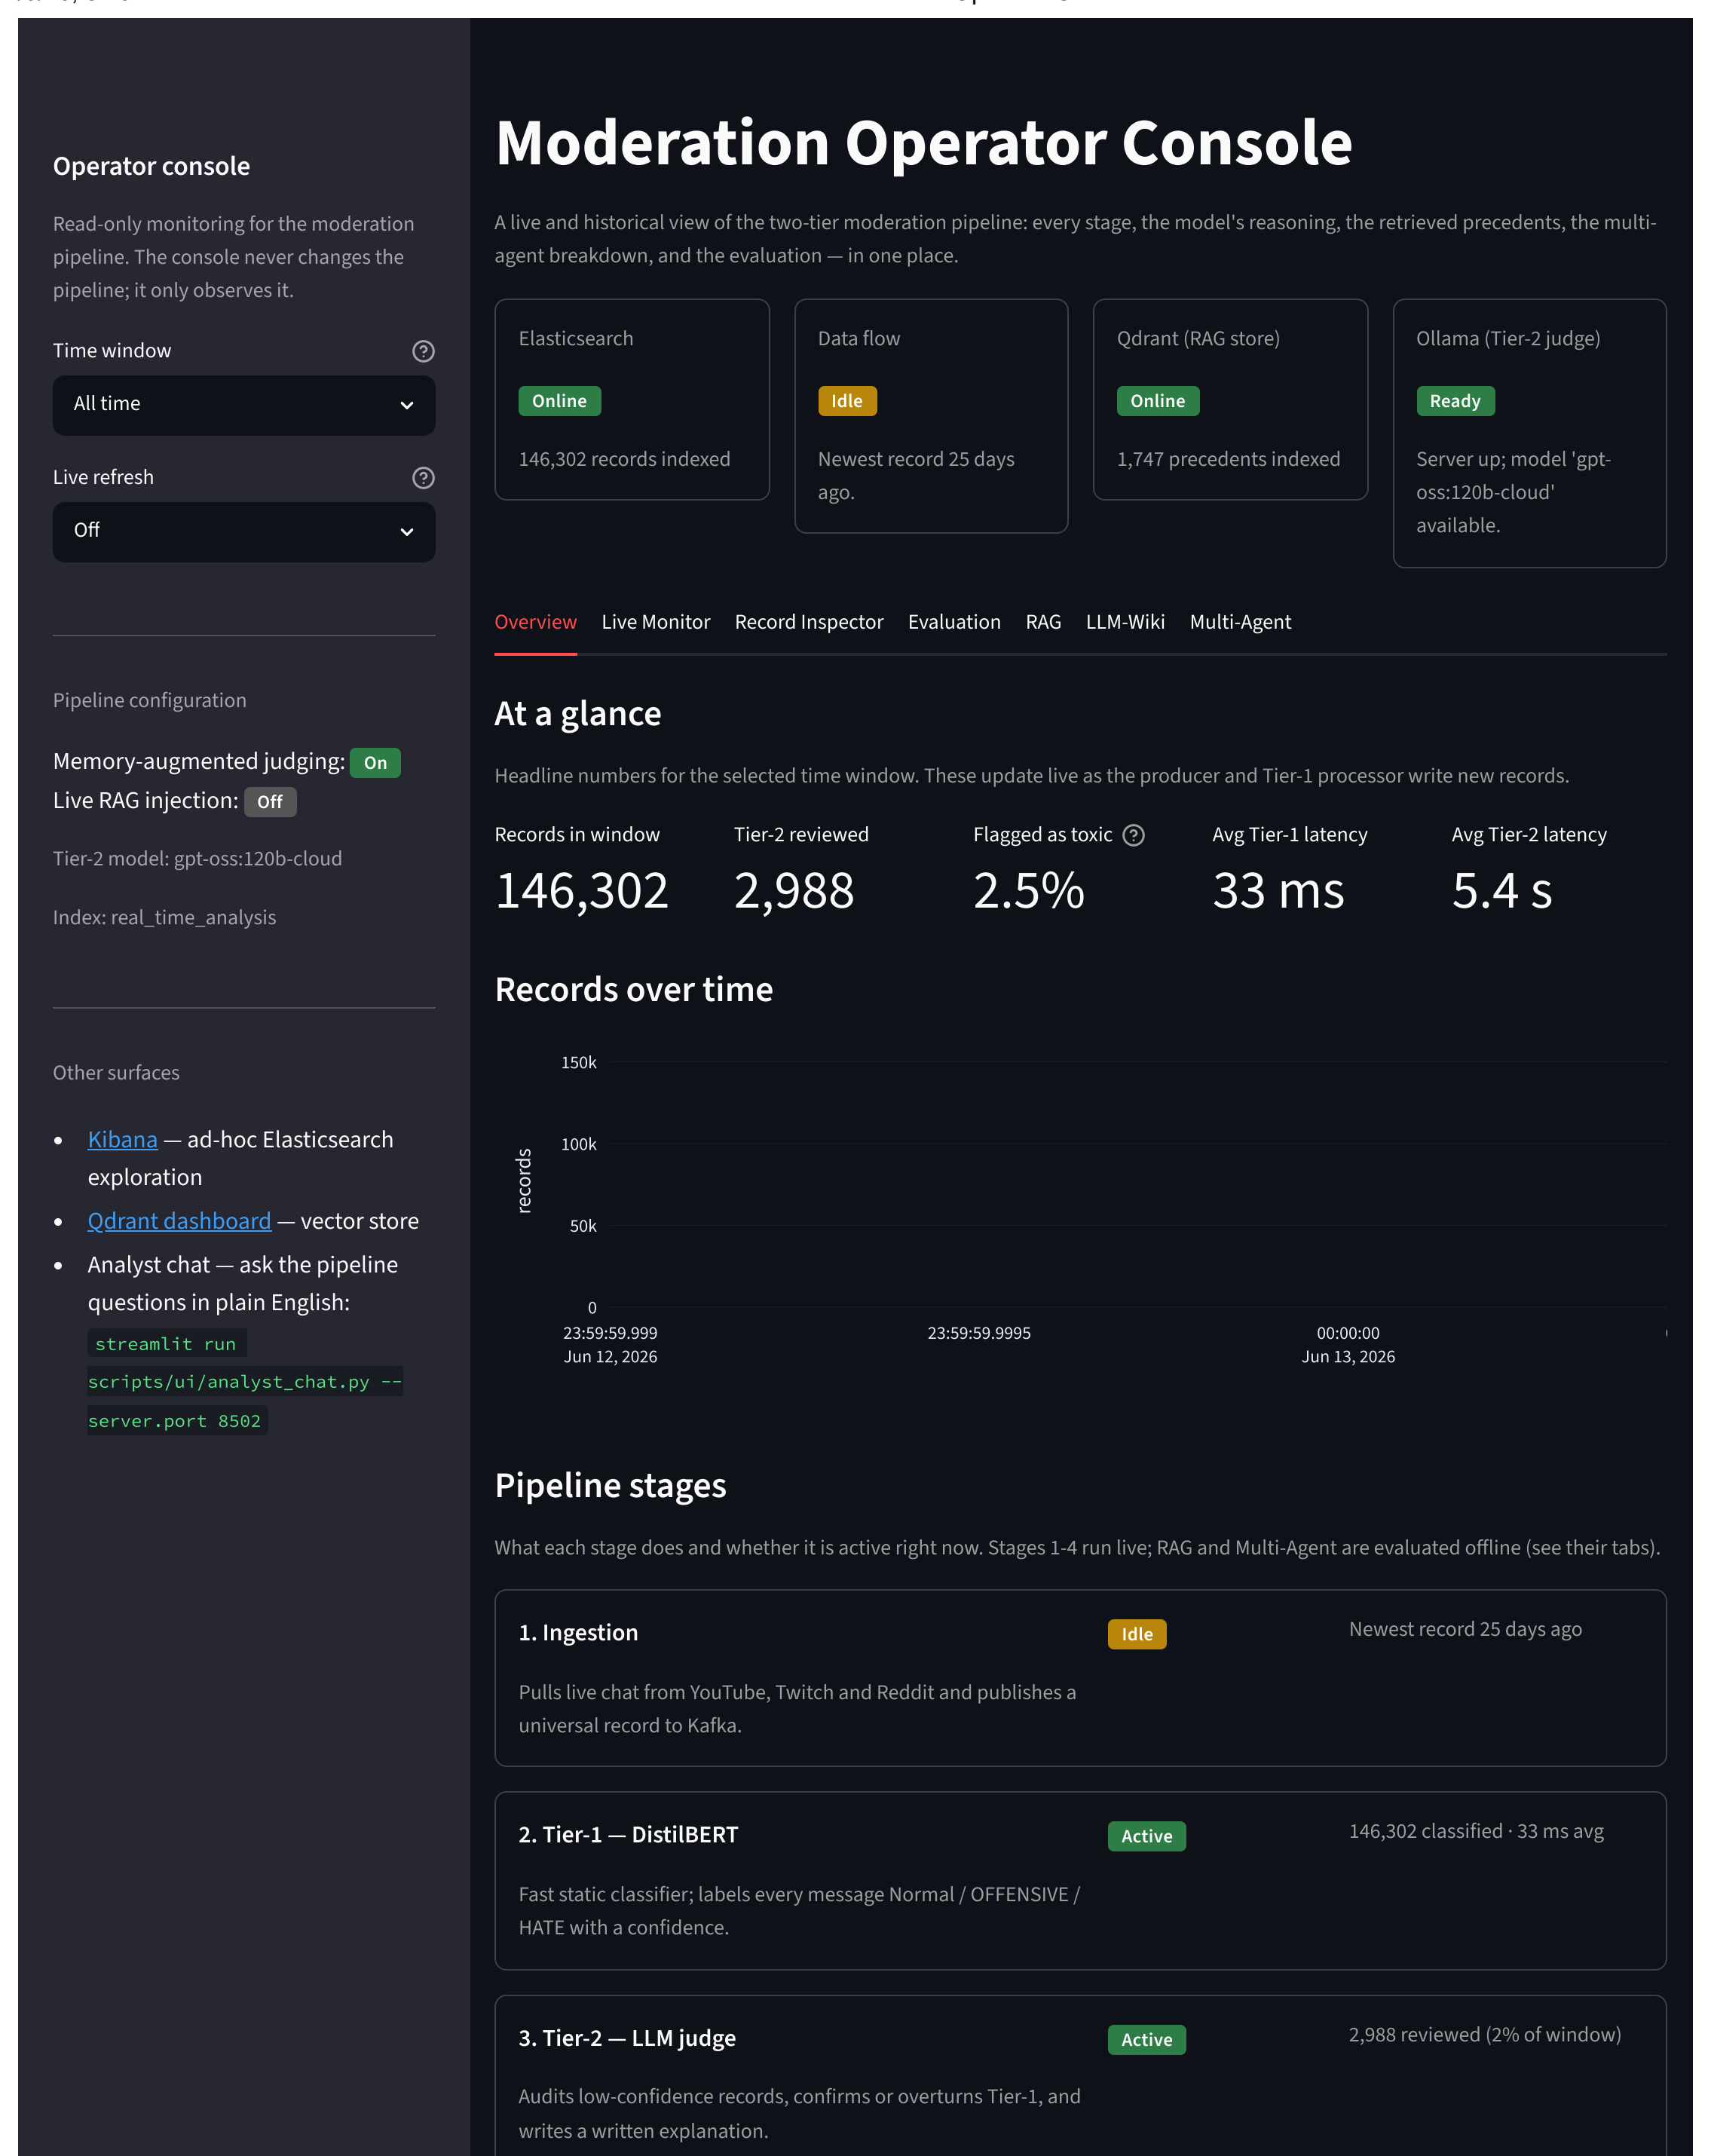
\includegraphics[width=1.5\linewidth,height=0.85\textheight,keepaspectratio]{figures/dashboard_overview.png}
\caption{The operator dashboard (Overview tab), built in Streamlit: the live status strip, the at-a-glance headline numbers, and the per-stage pipeline view.}
\end{figure}

\begin{figure}[H]
\centering
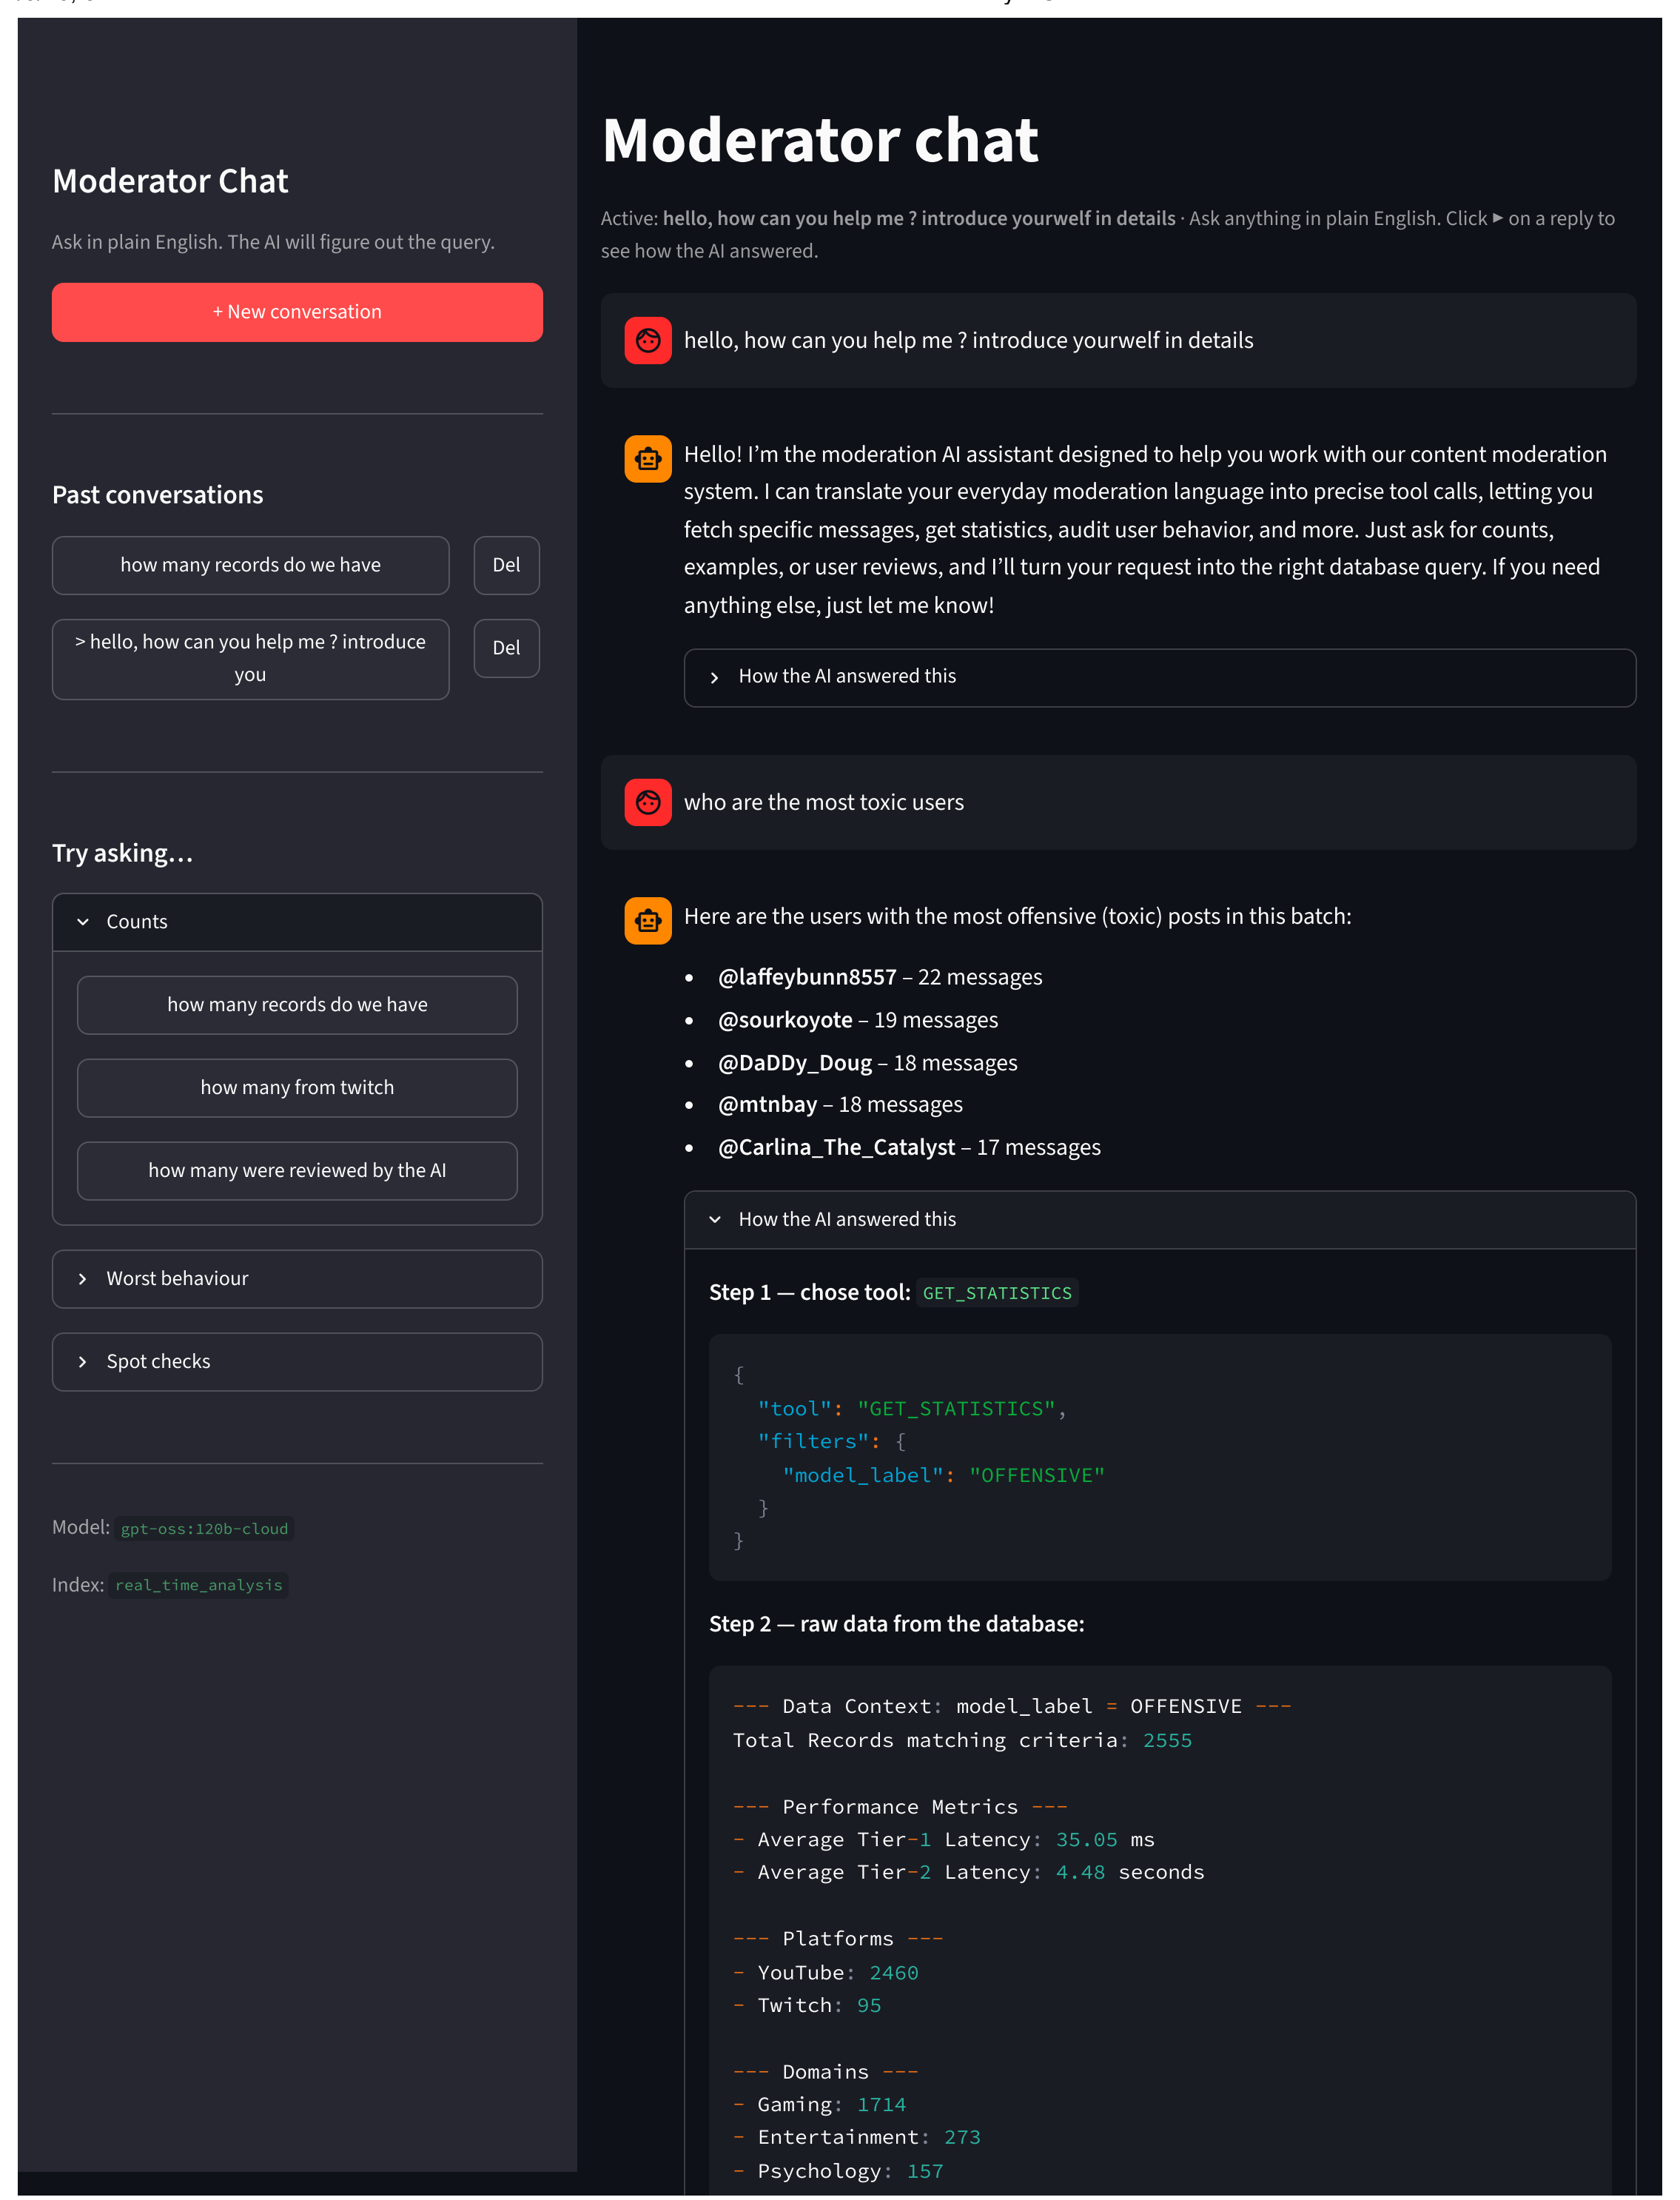
\includegraphics[width=1.5\linewidth,height=0.85\textheight,keepaspectratio]{figures/analyst_chat.png}
\caption{The natural-language analyst console: a plain-English question (``who are the most toxic users'') is turned into a tool call, and the expandable ``How the AI answered this'' panel shows the chosen tool and the raw data behind the reply.}
\end{figure}

\section{The Universal Schema}\label{the-universal-schema}

Two contracts hold the pipeline together. Keeping them apart was deliberate.

The first is the \textbf{Universal Kafka payload}, the shape every producer must emit and the processor consumes. It carries the message text, the source platform, the Context Agent's fields (domain, sub-genre, strictness, and the reasoning behind them), and a nested bag of platform-specific metadata: message and thread identifiers, author, role flags. Its one job is to guarantee the processor never breaks on a missing field. Anything a platform wants to add goes in the metadata bag, and nothing downstream has to care.

The second is the \textbf{Elasticsearch document}, which is what the processor writes and what the dashboards and agents read. It begins as the Tier-1 record, with identity, source context, author, and the DistilBERT prediction and its latency. Tier-2 then \emph{overlays} its verdict and explanation on top, and as the thesis progresses each variant gets its own named slot: memory, retrieval, multi-agent. Those slots never overwrite each other. That is what keeps the original baseline numbers reproducible no matter how many reasoning strategies get layered on afterwards.

Here i used two schemas instead of one shared object,Because producers and analysts care about genuinely different things. A producer has no business knowing a Tier-2 memory field exists. A dashboard should see exactly what is in storage and never an ingestion-side internal leaking through. The seam between the two is precisely where Tier-1 hands off to everything that follows.

\section{Deployment and reproducibility}\label{deployment-and-reproducibility}

The entire infrastructure is defined in a single \texttt{docker-compose} file, so anyone can stand it up and try it in their own environment.

Following the comparisons above, the final set of tools is: Kafka and Zookeeper for the broker, a Spark master and worker for distributed compute, Elasticsearch and Kibana for storage and visualisation, and Qdrant for vectors, all on one private network with persistent volumes.

The LLM is the only component outside that stack, reached through Ollama. A 120-billion-parameter judge does not fit the modest 4\,GB GPU the rest of the system was designed around, so the experiments reported here run \texttt{gpt-oss:120b} on Ollama's hosted endpoint. The same interface also serves a fully local model with no change to the pipeline, and that matters for more than convenience. A local open-weight model such as \texttt{dolphin-llama3} is not bound by the content policies that hosted providers apply, and those policies are a real obstacle in this field: a moderation system has to reason about the very language a general-purpose assistant is trained to refuse. Moving the judge on-premise, on adequate hardware, is therefore a one-line configuration change rather than a redesign, and it buys both privacy and freedom from a refusal that would otherwise arrive mid-evaluation.

\chapter{Methods and Implemented Modules}\label{methods-and-implemented-modules}

Chapter~\ref{system-architecture} described \emph{what} the pipeline is. This chapter is about \emph{how} each part works: the data it learns from, the two classifiers, the context modules layered on the second one, and the rules used to judge all of them. Every configuration value, model name, and threshold appears here, so each result can be traced back to the settings that produced it. The order follows the path a message takes, from the model that sees it first to the agents that argue over the hard cases.

\section{Overview}\label{overview}

Static models are far faster than language models. That single fact sets the shape of the method: Tier-1, the static model, handles the bulk of the traffic quickly, and the slow model is called in only for the cases that need more care.

What the slow model brings is context, which is exactly what the fast one lacks. Before it runs, that context is assembled in four ways, each built as its own module and each measured on its own: memory of what a user has done before, retrieval of similar past cases, a curated knowledge base, and a multi-agent chain that splits the decision across four specialised agents.

Because they sit behind a common interface, they can be switched on one at a time. That is what makes the comparison in Chapter~\ref{evaluation-and-results} a fair one rather than a tangle of confounded changes.

The chain is the same one the architecture used: question, requirement, choice, test. Where a section answers to a particular research question that is noted at its head, and the summary table in Chapter~\ref{evaluation-and-results} closes the loop for all three. Section~\ref{reproducibility-summary} then gathers every parameter named anywhere in this chapter into one table, so nothing has to be hunted for.

\section{Datasets}\label{datasets}

The project uses two datasets, and they do different jobs. One trains the fast classifier. The other tests the whole pipeline.

\textbf{Dataset A : the training corpus.} The training corpus holds 52,972 labelled comments merged from three established sources: Davidson et al., contributing 24,783 rows of informal, slang-heavy social media text \citep{davidson2017}; HateXplain, 19,229 rows with human rationales resolved by majority vote \citep{hatexplain2021}; and ToxiGen, 8,960 machine-generated rows carrying implicit, non-obvious toxicity \citep{toxigen2022}. The merge is deliberate, since each corpus covers a weakness the others leave open. Trained on all three, the model sees explicit slurs, subtle implicit hate, and everyday slang instead of one flavour of the problem. Labels are the three classes introduced in Chapter~\ref{state-of-the-art} (hate, offensive, and normal), and text is truncated at 128 tokens. That length was not arbitrary: it already covers the 95th percentile of comment lengths (Figure~\ref{fig:class-distribution}), so cutting there costs almost nothing.

\textbf{Dataset B : the evaluation benchmark.} Metrics come from a separate hand-labelled benchmark, not from held-out training data. The reason is that the object under test is the \emph{pipeline in context}, not a classifier on data resembling its own. So the benchmark is drawn from live records and labelled by hand into the same three classes. How those records were picked matters for reading the results, and it belongs here rather than in Chapter~\ref{evaluation-and-results}.

Drawing them at random would have been the simpler course, and it would have left almost nothing to measure. Toxic messages are thin on the ground in collected traffic to begin with, and thinner still because both platforms let a channel stop the worst of them before viewers see them. YouTube can hold the messages its system flags until the channel approves them, and Twitch's AutoMod holds flagged messages for moderator review, while a short chat delay, set in seconds, gives moderators time to remove a message before it appears \citep{youtubelivechat2026, twitchapi2026}. A pipeline that reads chat as a viewer never receives those messages. Section~\ref{limitations} takes up what that costs the study as a whole. The benchmark carries its own evidence for it: of the two hundred-odd records taken at random, not one proved toxic once a human had read it.

The selection is therefore weighted. Records are scored for how much they are worth labelling by hand, with weight given to three things: a toxic Tier-1 prediction, a disagreement between the two tiers, and low Tier-1 confidence. The sampler reserves a quarter of its quota for records taken at random from the confidently-normal majority and fills the rest from the top of that ranking, so the judge is also scored on cases it ought to leave alone. In the finished benchmark that random share came to 204 of the 1,748 records. Weighting is what put eighty positives in the set at all, and it is the same choice that stops the set standing in for ordinary traffic. What it could not remove is the rarity of toxic content itself, and that rarity is why raw accuracy is set aside in favour of toxic-class metrics, as Section~\ref{evaluation-methodology} explains.

\begin{figure}[H]
\centering
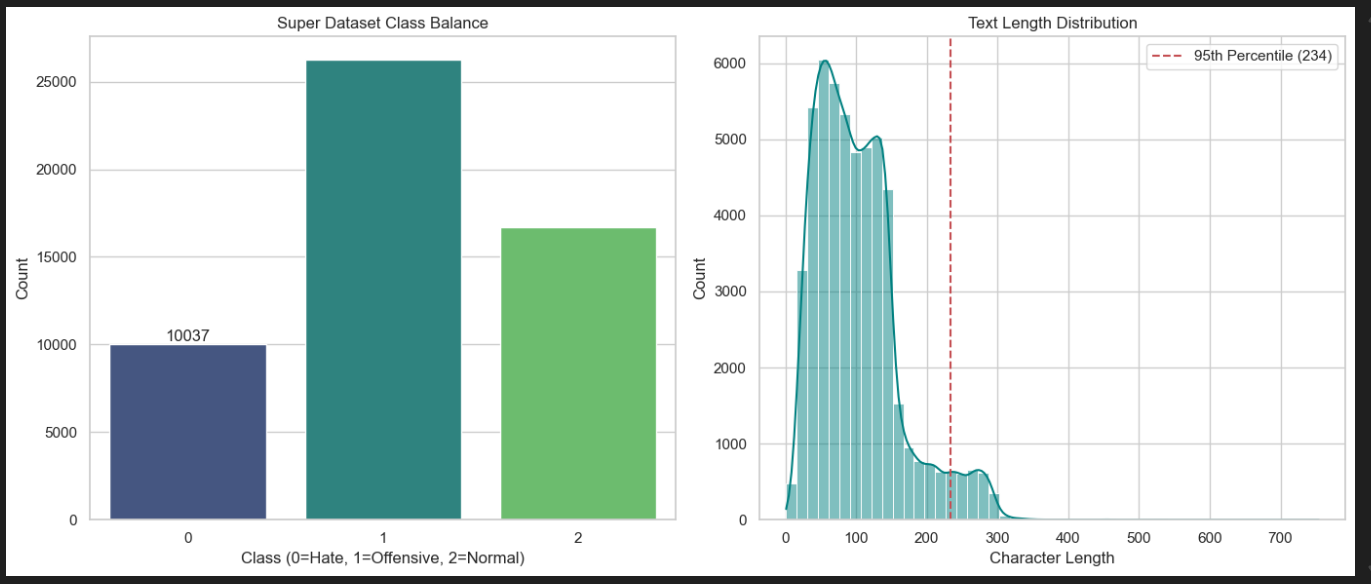
\includegraphics[width=1\linewidth,height=0.85\textheight,keepaspectratio]{figures/class_distribution.png}
\caption{Dataset A. Left: the three-class balance of the 52,972-message training corpus (offensive is the majority class, hate the smallest). Right: the character-length distribution, with the 95th percentile at 234 characters, which is why inputs are truncated at 128 tokens with almost no loss.}\label{fig:class-distribution}
\end{figure}

\section{Tier-1: the fast static classifier}\label{tier-1-the-fast-static-classifier}

\emph{Two questions meet here. Tier-1 has to be quick enough to carry RQ1's real-time claim, and wrong in the particular way that leaves RQ2 something worth correcting.}

Speed is the constraint this model is chosen around, because it has to keep up with a live stream.

\textbf{Classical baselines.} Two simpler models set the bar. A Logistic Regression and a linear SVM, both over TF-IDF features, trained on all 52,972 messages, split 80/20 with a fixed random seed. They are cheap, need no GPU, and land at 75.6 and 75.0 per cent accuracy on the 10,595 held-out messages. Their real value is as a control: they show how far plain word-counting gets, and therefore how much the transformer actually adds. Where they fail is any case that turns on meaning rather than vocabulary, a reclaimed slur used affectionately, or sarcasm that inverts what the words say, because a bag of TF-IDF weights has no way to represent ``this word means the opposite of what it usually does here.''

\textbf{DistilBERT.} The chosen Tier-1 model is a fine-tuned \texttt{distilbert-base-uncased}, a six-layer distilled transformer that keeps most of BERT's language understanding at a fraction of its size and latency \citep{distilbert2019}.

The choice was as much about hardware as about the model, and the arithmetic is worth showing rather than asserting. Everything here was trained and run on a laptop with 12 GB of system memory and a GPU carrying 4 GB of video memory. The fine-tuned Tier-1 model holds 67.0 million parameters across six layers and takes about 269 MB on disk. BERT-base, and with it HateBERT, which keeps BERT's architecture, holds 110 million across twelve layers, roughly 1.6 times as many. Fine-tuning costs more than the weights, though: it needs the weights plus their gradients, plus the optimiser's two moment estimates per parameter, plus the activations held for the backward pass. The working requirement is several times the model size, and at that multiple the larger encoder leaves no workable headroom in 4 GB. The same ceiling is why the training batch size is 8 rather than the conventional 32.

Training itself is unremarkable: two epochs, weight decay 0.01, 100 warm-up steps, and sequences padded and truncated to 128 tokens, with the optimiser and learning rate left at the library defaults of AdamW and 5e-5. To keep fine-tuning time manageable on the laptop GPU, DistilBERT was trained on a random sample of 43,000 of the 52,972 messages rather than on all of them, split 80/20 into 34,400 for training and 8,600 for evaluation. That split was drawn without a fixed seed, so its exact partition cannot be regenerated. Appendix~\ref{hardware-and-software-environment} lists the full environment.

On its 8,600 evaluation messages the model reaches about 79 per cent accuracy and F1 around 0.80, a few points above the classical baselines. Because the baselines were scored on a different held-out set, that gap is indicative rather than exact. The like-for-like comparison is the set of 500 live messages described below, which all three models labelled: on the toxic class, DistilBERT reaches an F1 of 0.38, against 0.27 for Logistic Regression and 0.24 for the SVM. But accuracy is not why it was picked. Latency is. DistilBERT labels a message in roughly 31 milliseconds on this hardware (Section~\ref{latency-and-computational-cost}), which is what lets it sit in front of a live stream without adding lag anyone would notice (throughput is measured in Section~\ref{throughput-scalability}).

Each prediction is a soft-max over the three classes. The highest-scoring class becomes the label, and its probability is the \emph{confidence} that decides whether the second tier is needed (Section~\ref{tier-2-the-llm-judge}).

Figure~\ref{fig:bert-confusion} shows the model's real weakness, and it is the whole reason a second tier exists. The set is 500 messages from a single YouTube stream, labelled by hand and collected separately from the Chapter~\ref{evaluation-and-results} benchmark. DistilBERT gets almost all the normal traffic right, 435 of 452. Then it collapses on the toxic classes. Of 25 genuinely offensive messages it calls 23 of them normal, and it scatters the hate class across all three labels. A model this blind to toxicity in context is a useful fast filter and nothing more, which is exactly the role it is given.

\begin{figure}[H]
\centering
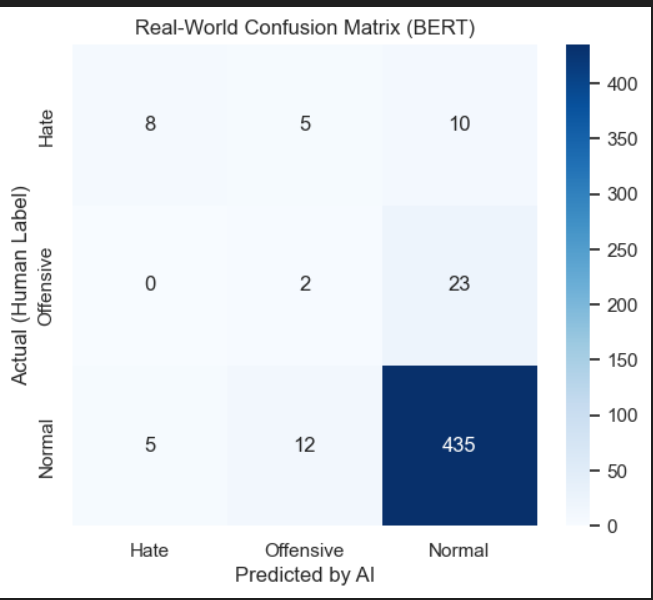
\includegraphics[width=0.9\linewidth,height=0.85\textheight,keepaspectratio]{figures/bert_confusion_matrix.png}
\caption{DistilBERT confusion matrix on 500 hand-labelled messages from one YouTube stream (actual human label vs.~predicted). The model handles normal content well but misreads most toxic messages as normal, motivating the Tier-2 judge.}\label{fig:bert-confusion}
\end{figure}

\section{The Context Agent}\label{the-context-agent}

Before a message is classified at all, the pipeline works out what kind of place it came from.

The naive way would be to hand the model a fixed menu of categories and make it choose. That turns discovery into guesswork the moment a stream fits nothing on the menu. So the Context Agent does the opposite: it asks an LLM to read the stream's metadata, its title, channel, and description, and describe in free text what the stream is about and how strictly it should be moderated. A live esports final comes back as gaming, low strictness, because aggression is expected there. A political broadcast comes back high.

That free-text answer is then normalised onto a stable set of canonical domains (Figure~\ref{fig:context-agent}) so the downstream analytics stay consistent, and the model's original wording is kept beside it. Keeping the raw proposal matters twice over. It is auditable, and it is itself a finding, a record of the categories the model reached for unprompted, including ones outside the seed list. On the benchmark those are common: 628 of the 1,748 records, 36 per cent, carry a domain the seed list did not contain. If the LLM call fails, the agent falls back to safe defaults instead of blocking ingestion, so a hiccup in the reasoning layer never stops the stream.

There is a further consequence, and it is the reason this design was chosen over a fixed list. The canonical domains live in an operator-editable file, \texttt{config/taxonomy.yaml}, not in the code, and every off-list proposal is logged rather than discarded. When a new game, a new platform, or a fresh piece of slang starts appearing, an operator watches it accumulate in those logs and promotes it into the taxonomy without touching a line of Python. The system's sense of context can therefore follow trends as they emerge, which matters a great deal in a setting where the vocabulary of both ordinary speech and abuse keeps shifting. A taxonomy frozen at training time would be stale within months. This one grows with the platforms it watches, and that adaptability is part of what the ``agentic'' claim is meant to deliver.

\begin{figure}[H]
\centering
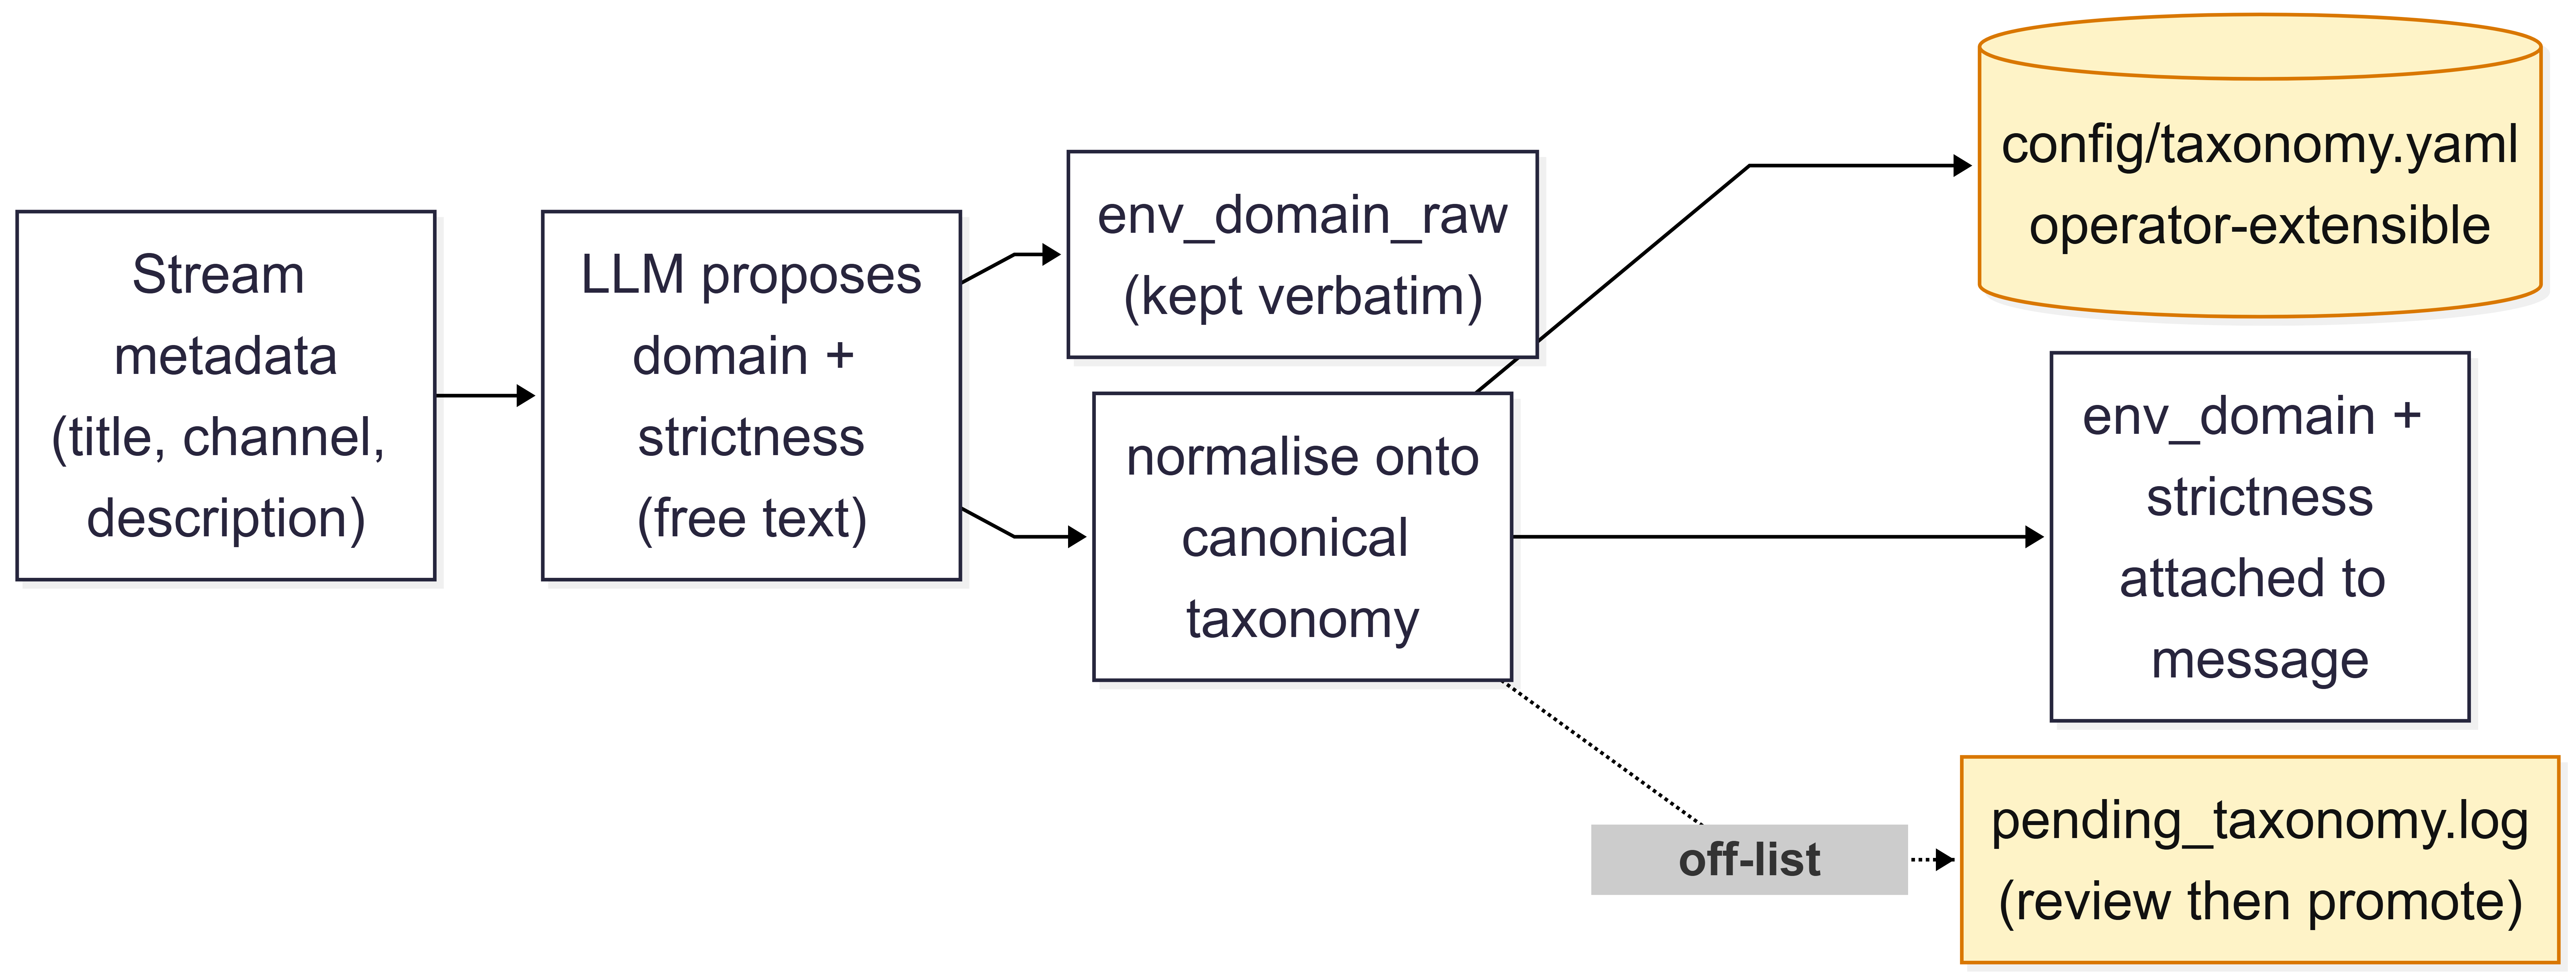
\includegraphics[width=0.9\linewidth,height=0.85\textheight,keepaspectratio]{figures/contextAgent.png}
\caption{The Context Agent: agentic discovery of domain and strictness, then normalisation onto the operator-extensible taxonomy.}\label{fig:context-agent}
\end{figure}

\section{Tier-2: the LLM judge}\label{tier-2-the-llm-judge}

The second tier is where context finally enters the decision. It is a large language model, \texttt{gpt-oss:120b}, an open-weight mixture-of-experts model with 116.8 billion parameters, of which 5.1 billion are active for any one token \citep{gptoss2025}, reached through Ollama under the tag \texttt{gpt-oss:120b-cloud} and used as a judge in the sense of the LLM-as-a-judge literature \citep{llmjudge2023}. The experiments here reach it on Ollama's hosted endpoint, since a model that size will not fit a 4\,GB GPU, but the same interface serves a fully local model such as \texttt{dolphin-llama3} unchanged where the hardware allows.

What it does is narrow. It reads the message, the Tier-1 verdict and its confidence, and the stream's context, then returns one of three verdicts, that Tier-1 was correct, that it was a false positive, or that it was a false negative, along with a written explanation.

Two choices make it behave like a classifier instead of a chatbot. Inference is pinned to temperature zero, so the same input gives the same verdict as nearly as a hosted endpoint allows, since its batching and hardware sit outside the pipeline's control. And the model must return structured JSON, so its output parses without guesswork, with one automatic retry if it ever strays. The explanation is not decoration. It is what lets a human moderator see the reasoning behind an overturned decision, which a bare probability from Tier-1 could never provide.

The judge, on the other hand, is expensive, so it is rationed. It runs only on messages Tier-1 was unsure about, confidence below 0.80, and it runs asynchronously (Figure~\ref{fig:two-tier}), reading its work from storage rather than sitting in the live path. The effect is the one the whole architecture is built around: the model that takes seconds never touches the model that takes milliseconds. It is the difference between answering every email the moment it lands and setting the awkward ones aside for a batch later. The inbox never backs up because of the slow ones. That is the deployed behaviour; the single place where the evaluation departs from it is recorded in Section~\ref{evaluation-methodology}.

One thing about that threshold should be said plainly. The 0.80 figure is a design parameter, not a tuned one. It was fixed before any evaluation, as a round value that pushes clearly-uncertain cases upward while leaving the confident majority alone, and no sweep across candidate thresholds was run to find the value that maximises any particular metric. Which direction the trade runs is easy enough to see: lower the gate and the judge reviews less traffic and misses more of the hard cases, raise it and the reverse happens at greater cost. Where that curve actually turns is left open. Answering it properly would take a calibration study across a range of thresholds, measuring cost against toxic-class recall at each, and that is a study this thesis does not attempt.

Every prompt used here is reproduced verbatim in Appendix~\ref{prompt-library}.

\begin{figure}[H]
\centering
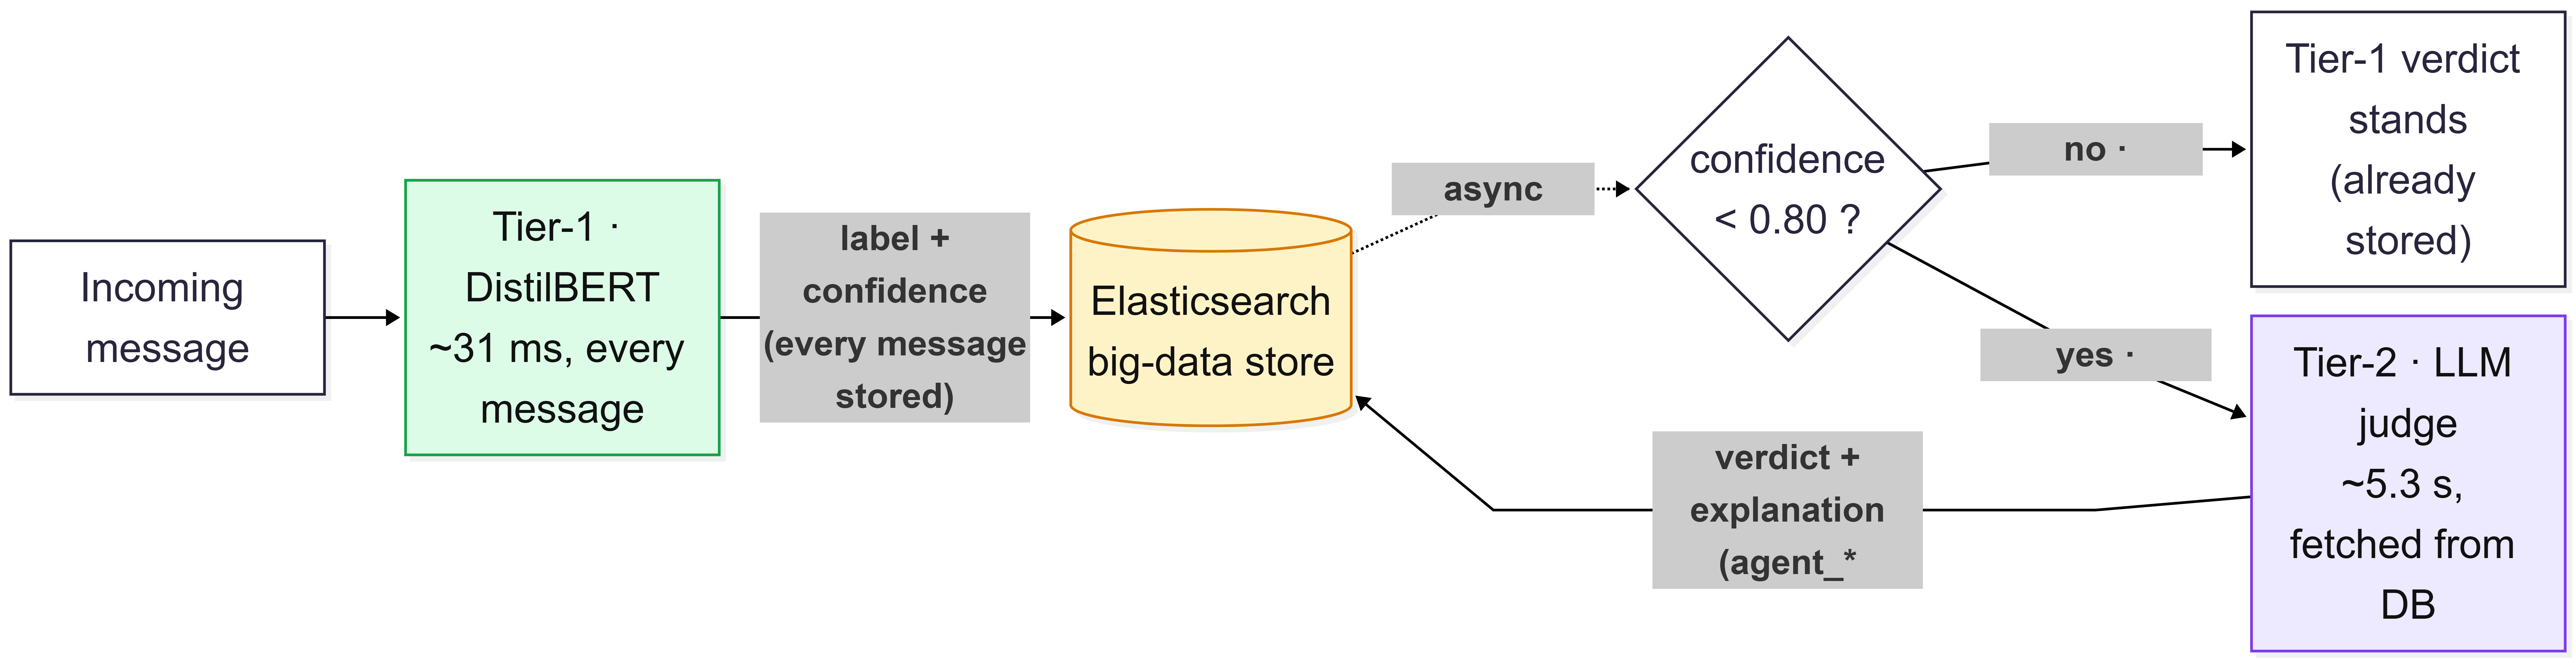
\includegraphics[width=0.95\linewidth,height=0.85\textheight,keepaspectratio]{figures/two_tier_flow.png}
\caption{The two-tier design: a fast static classifier with a confidence gate that escalates only the uncertain minority to the slow LLM judge, asynchronously.}\label{fig:two-tier}
\end{figure}

\section{Temporal memory}\label{temporal-memory}

\emph{The next four sections take the context mechanisms in turn. Each is built to be switched off without disturbing the others, which is what lets RQ3 be answered module by module instead of in aggregate.}

A single message is thin evidence. The same three words can be a shrug or a threat depending on who typed them and what came just before, and Tier-2 on its own sees only the isolated line.

The memory module fixes that by pulling three things out of storage before the judge decides (Figure~\ref{fig:temporal-memory}): the author's recent messages, the last few messages in the same thread, and a short behavioural fingerprint summarising how often that author has been normal, offensive, or hateful lately.

The intuition behind it is ordinary. A regular who has posted a hundred harmless messages and then writes something borderline is probably joking. The same line from an account flagged twice this week reads differently. A moderator who knew both histories would treat them differently, and memory gives the judge that history.

It is bounded on purpose, so the prompt stays a sensible size and old behaviour does not drown out the present. The judge sees the author's last ten messages from the past twenty-four hours, the five messages that came just before this one in the same thread, and a fingerprint computed over the author's last twenty labelled messages from the same twenty-four hours. All four windows are configuration values rather than constants in the code, so any of them can be widened or narrowed without touching the pipeline.

\begin{figure}[H]
\centering
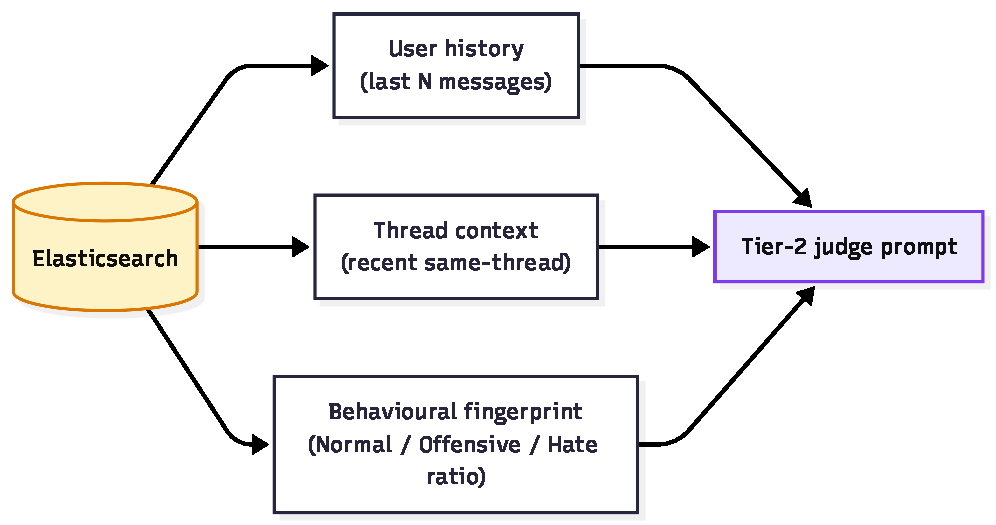
\includegraphics[width=0.9\linewidth,height=0.85\textheight,keepaspectratio]{figures/temporal_memory.pdf}
\caption{Temporal memory: the user history, thread context, and behavioural fingerprint pulled from Elasticsearch into the judge prompt.}\label{fig:temporal-memory}
\end{figure}

\section{Retrieval-augmented moderation (RAG)}\label{retrieval-augmented-moderation-rag}

Memory looks at the \emph{author}. Retrieval looks at \emph{other, similar cases}.

The RAG module embeds the current message into a 384-dimensional vector using a compact sentence-transformer, \texttt{all-MiniLM-L6-v2} \citep{sbert2019}, then asks a Qdrant vector database for the five past messages whose vectors sit closest by cosine similarity, keeping only those above 0.55. Those nearest cases, with the verdicts they received, go to the judge as precedent, following the retrieval-augmented pattern \citep{rag2020}.

Think of it as case law. Faced with an ambiguous message, the judge is shown how comparable messages were handled before, and can lean on that consistency instead of deciding from scratch each time. For evaluation the retrieval is leave-one-out, so the current message is always excluded from its own results and can never retrieve itself to inflate the score. The embedder, the neighbour count of five, and the 0.55 threshold all live in one file, \texttt{config/rag.yaml}, so swapping the embedder is a one-line change.

\section{The LLM-Wiki backend and the switchable interface}\label{the-llm-wiki-backend-and-the-switchable-interface}

RAG grounds the judge in past \emph{cases}. The LLM-Wiki grounds it in curated \emph{knowledge}. Setting those two against each other is one of the experiments this thesis was built to run.

Where RAG retrieves whatever the corpus happens to hold, the Wiki reads from a small hand-written knowledge base: a core policy page defining the three labels; rule pages for gaming, for politics and news, and for reviews, with a general page for every other domain; a glossary of coded language and evasion tricks; and a set of edge-case rulings covering reclaimed slurs, sarcasm, and quoting without endorsing. For any given message the module always supplies the core policy and that message's domain page, then adds the most relevant glossary or edge-case entries, found using the same embedder RAG uses. Keeping the encoder identical was deliberate. Both backends then judge relevance the same way, so the main difference between them is \emph{what} gets retrieved, curated rules or past examples, and that keeps the comparison as clean as two different corpora allow.

That decision is also where this implementation parts company with the pattern it borrows. At the scale Karpathy describes, a hundred or so sources, the wiki needs no retrieval at all: an index page tells the model which files to open and they go straight into the context window, with search recommended only once a collection outgrows that \citep{karpathy2026llmwiki}. The knowledge base here is smaller still, so loading it directly would have served perfectly well. It is indexed anyway, and the reason is methodological rather than technical. Reading the pages straight into the prompt would have changed two variables at once, the corpus and the means of reaching it, leaving no way to attribute any difference in the results to either. Reusing RAG's encoder holds the means of retrieval constant, so the corpus is the main thing that varies, although each backend keeps its own count and cut-off. The knowledge base's eight content pages are split at every second-level heading into 34 entries, a ninth page serving only as navigation and carrying no knowledge of its own. Those entries are embedded once with the same MiniLM encoder and held in memory, and a query returns the four most relevant above a cosine similarity of 0.15, on top of the policy and domain pages that are always included. Those values live in \texttt{config/wiki.yaml}. The threshold sits well below RAG's 0.55 on purpose, because a policy page is relevant to a message in a much looser sense than a near-duplicate past case is, and holding both to the same bar would starve the Wiki of anything to say.

Each is good at a different kind of case. A coded phrase like a ``great replacement'' dog-whistle rarely has a close neighbour among past messages, so RAG may return nothing useful, while the Wiki's glossary names it outright. The trade runs the other way for a message whose meaning lives in one very specific prior case that no policy page anticipated.

Both sit behind a single interface, \texttt{retrieval.py}, and one configuration flag, \texttt{RETRIEVAL\_BACKEND}, picks between them (Figure~\ref{fig:retrieval-backends}): \texttt{rag}, \texttt{wiki}, or \texttt{none}. Switching the live pipeline from vector retrieval to the knowledge base is one line, with nothing else touched. That is the concrete meaning of the switchable backend this thesis claims. A graph-structured variant, GraphRAG, is left as future work.

\begin{figure}[H]
\centering
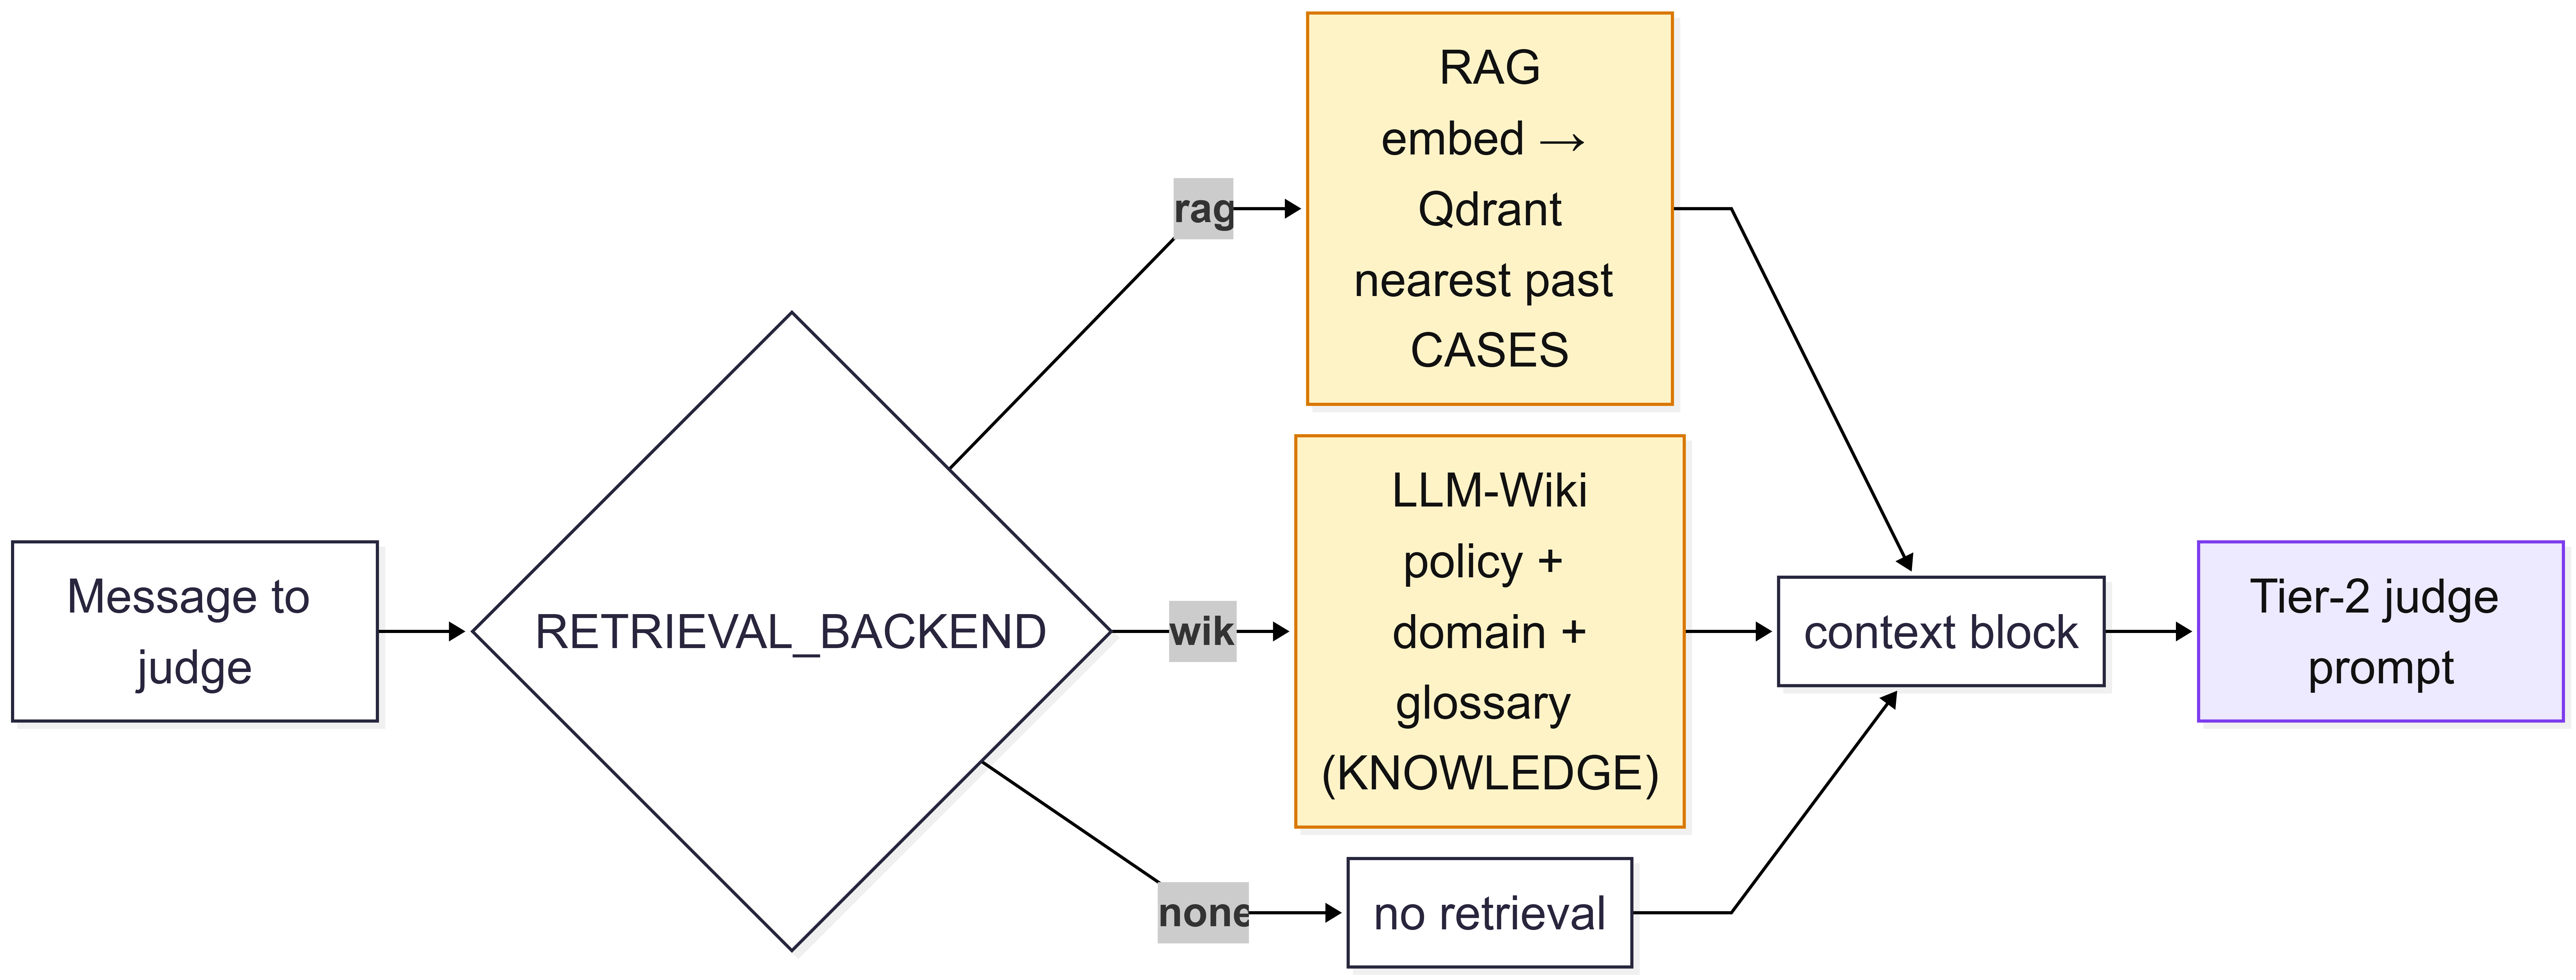
\includegraphics[width=0.9\linewidth,height=0.85\textheight,keepaspectratio]{figures/retrieval_backends.png}
\caption{The switchable retrieval backend: a single flag selects RAG (nearest past cases) or the LLM-Wiki (curated knowledge), feeding the same judge prompt slot.}\label{fig:retrieval-backends}
\end{figure}

\section{The multi-agent chain}\label{multi-agent-decomposition}

So far the judge is one call doing everything at once: reading the content, weighing the author, deciding. The multi-agent chain breaks that into four smaller calls, each with a narrow job, run in sequence (Figure~\ref{fig:multi-agent}).

\begin{enumerate}
\def\labelenumi{\arabic{enumi}.}
\tightlist
\item \textbf{Risk Scorer} reads only the message content and rates its toxicity from 0 to 1, with no knowledge of who sent it.
\item \textbf{Behaviour Profiler} reads only the author's history and rates the account low, medium, or high risk, with no knowledge of the current message.
\item \textbf{Escalator} takes those two signals and decides how to route the case (clear it automatically, flag it automatically, or send it to a human).
\item \textbf{Supervisor} reads everything the others produced and issues the final verdict in the same three-way format as every other variant (Tier-1 correct, false positive, or false negative), so it stays directly comparable.
\end{enumerate}

Why split a job one prompt could do? For the same reason a newsroom separates the reporter from the editor. When one person does both, a mistake afterwards is impossible to place, in the facts or in the judgement. Separate the steps and each one leaves a record. If the final verdict is wrong, the stored risk score, behaviour rating, and routing decision show which step went astray, and that per-step trace is what the dashboard's Multi-Agent tab displays and what Section~\ref{inside-the-multi-agent-chain} analyses. The cost is four LLM calls per message instead of one, which is affordable only because, like the rest of Tier-2, this runs on the flagged minority alone.

\begin{figure}[H]
\centering
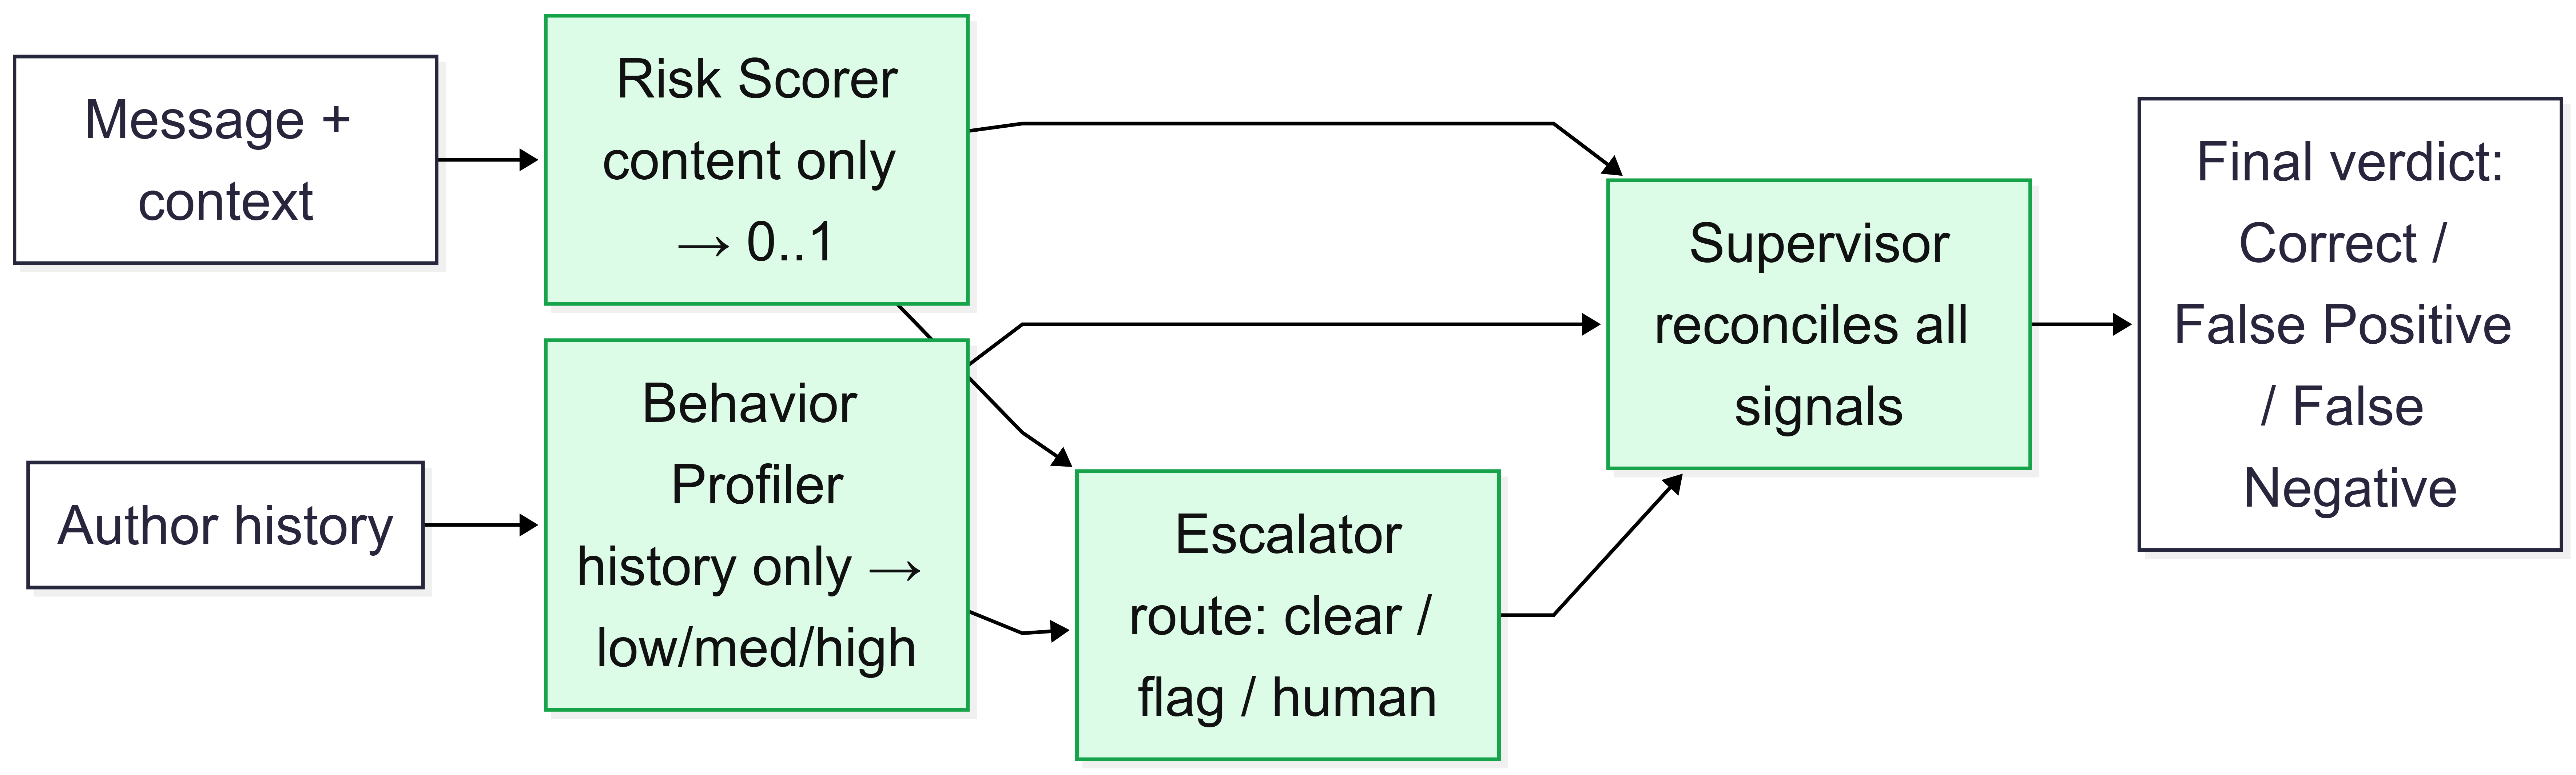
\includegraphics[width=0.9\linewidth,height=0.85\textheight,keepaspectratio]{figures/Multi-agent.png}
\caption{The multi-agent chain: the Risk Scorer and Behaviour Profiler feed an Escalator and a Supervisor that issues the final verdict.}\label{fig:multi-agent}
\end{figure}

\section{Evaluation methodology}\label{evaluation-methodology}

One departure from the live configuration should be recorded before anything else. In deployment the confidence gate decides what the judge ever sees; for the evaluation it was set aside, and every variant judged all 1,748 records whatever Tier-1's confidence had been. That is what lets the configurations be compared on identical rows rather than on whichever subset each happened to receive, and it is also what makes the control group meaningful, since those confident cases are precisely the ones a judge should decline to overturn.

The rest of the method is shaped by one awkward fact: toxic content is rare, in live traffic and in this benchmark alike. A model that labelled everything ``normal'' would score 95.4 per cent accuracy here and catch not one toxic message. Raw accuracy here is not merely unhelpful. It is actively misleading, because reporting it would reward the model for doing nothing.

So the evaluation leads with the toxic class. Every variant is reported with precision, recall, and F1 on hate-plus-offensive content, alongside confusion matrices showing exactly where the errors land, with three-class and binary accuracy kept as secondary figures only. To put the variants on equal footing, their different verdict formats are first mapped to a common label: a ``correct'' verdict keeps Tier-1's label, a ``false positive'' becomes normal, a ``false negative'' becomes toxic. Because a false-negative verdict does not say which toxic class was missed, the three-class accuracy counts it as offensive. A memory verdict and a multi-agent verdict can then be scored the same way against the same ground truth. Finally, since differences between variants can be small on a benchmark holding few toxic cases, each pairwise difference is tested with McNemar's test, in its continuity-corrected form, the standard paired test for two classifiers on one dataset \citep{mcnemar1947, dietterich1998}. McNemar's test counts every verdict, so it measures overall correctness, which the normal majority dominates; the toxic-F1 difference is therefore also given a paired bootstrap confidence interval \citep{efron1993}. Together they are what separate a real improvement from a lucky one, and it runs throughout Chapter~\ref{evaluation-and-results}.

\section{Summary of settings and parameters}\label{reproducibility-summary}

The settings behind the results appear above, next to the arguments that motivate them. Table~\ref{tab:params} gathers all of them in one place, so no setting has to be hunted for in the chapter or in the source. Where a value was forced by the hardware or chosen for a particular reason, the text gives that reason, and library defaults are named as such. None of the thresholds, though, were arrived at by sweeping a range and keeping whichever score came out highest. They are design settings, the confidence gate and the two retrieval cut-offs alike, and the text says so where each is introduced.

Three things complete the picture. Every prompt, for the Context Agent, the judge, and each of the four agents, appears verbatim in Appendix~\ref{prompt-library}, because a prompt shapes a result as surely as a learning rate does. The hardware and software environment, down to package versions and container tags, is in Appendix~\ref{hardware-and-software-environment}. And the whole stack comes from one \texttt{docker-compose} file, so the same Kafka, Spark, Elasticsearch, and Qdrant start with a single command, after which the evaluation scripts run against the same benchmark file.
\renewcommand{\arraystretch}{1.5} 

\begin{longtable}{@{}
  >{\raggedright\arraybackslash}p{\dimexpr 0.22\linewidth - 1.6\tabcolsep \relax}
  >{\raggedright\arraybackslash}p{\dimexpr 0.30\linewidth - 1.6\tabcolsep \relax}
  >{\raggedright\arraybackslash}p{\dimexpr 0.26\linewidth - 1.6\tabcolsep \relax}
  >{\raggedright\arraybackslash}p{\dimexpr 0.22\linewidth - 1.6\tabcolsep \relax}@{}}
\caption{Every configuration value behind the reported results, with where it is set.}\label{tab:params}\tabularnewline
\toprule
\textbf{Component} & \textbf{Setting} & \textbf{Value} & \textbf{Where set} \\
\midrule
\endfirsthead
\toprule
\textbf{Component} & \textbf{Setting} & \textbf{Value} & \textbf{Where set} \\
\midrule
\endhead
\bottomrule
\endlastfoot

Tier-1 model & base checkpoint & \texttt{distilbert-\allowbreak base-\allowbreak uncased} & \texttt{models/\allowbreak bert\_final} \\
 & training data & random sample of 43,000 of the 52,972 messages & training notebook \\
 & epochs / batch size & 2 / 8 & training notebook \\
 & optimiser & AdamW, lr 5e-5 (both library defaults), weight decay 0.01, 100 warm-up steps & training notebook \\
 & max sequence length & 128 tokens & training and inference \\
 & checkpoint directory & \texttt{models/bert\_final} & \texttt{MODEL\_DIR} \\
 & inference device & CPU by default, GPU selectable & \texttt{DEVICE} \\
 & train/evaluation split & 80/20; seeded for the baselines, unseeded for DistilBERT & training notebook \\
\addlinespace[1em]

Confidence gate & escalate to Tier-2 below & 0.80 (design choice, not calibrated) & processor \\
\addlinespace[1em]

Tier-2 judge & model & \texttt{gpt-oss:120b-\allowbreak cloud} via Ollama & \texttt{OLLAMA\_MODEL} \\
 & temperature & 0 (near-deterministic on a hosted endpoint) & judge call \\
 & output format & structured JSON, one retry on parse failure & judge call \\
\addlinespace[1em]

Temporal memory & author history window & 10 messages & \texttt{MEMORY\_\allowbreak USER\_\allowbreak WINDOW\_\allowbreak SIZE} \\
 & thread context window & 5 messages & \texttt{MEMORY\_\allowbreak THREAD\_\allowbreak WINDOW\_\allowbreak SIZE} \\
 & look-back (author history and fingerprint) & 24 hours & \texttt{MEMORY\_\allowbreak LOOKBACK\_\allowbreak HOURS} \\
 & fingerprint window & 20 messages & \texttt{MEMORY\_\allowbreak FINGERPRINT\_\allowbreak WINDOW} \\
\addlinespace[1em]

RAG & embedding model & \texttt{all-MiniLM-L6-v2}, 384 dimensions & \texttt{config/rag.yaml} \\
 & neighbours retrieved & 5 & \texttt{config/rag.yaml} \\
 & similarity threshold & 0.55, cosine & \texttt{config/rag.yaml} \\
 & self-exclusion & on (leave-one-out) & \texttt{config/rag.yaml} \\
\addlinespace[1em]

LLM-Wiki & embedding model & identical to RAG, by design & \texttt{config/rag.yaml} \\
 & knowledge base & 8 content pages, 34 entries split at second-level headings & \texttt{wiki/} \\
 & always supplied & core policy plus the domain page & \texttt{config/\allowbreak wiki.yaml} \\
 & entries retrieved & 4 & \texttt{config/\allowbreak wiki.yaml} \\
 & similarity threshold & 0.15, cosine & \texttt{config/\allowbreak wiki.yaml} \\
\addlinespace[1em]

Retrieval backend & selector & \texttt{rag} / \texttt{wiki} / \texttt{none} & \texttt{RETRIEVAL\_\allowbreak BACKEND} \\
\addlinespace[1em]

Multi-agent & calls per message & 4, run in sequence & agent chain \\
 & risk score range & 0 to 1, continuous & Risk Scorer \\
 & behaviour rating & low / medium / high & Behaviour Profiler \\
 & routing actions & auto\_clear / auto\_flag / human\_review & Escalator \\
 & failure handling & defaults to \texttt{human\_review} on a parse failure & agent chain \\
\addlinespace[1em]

Kafka & topic / partitions / replication & \texttt{universal\_stream} / 1 / 1 & \texttt{docker-\allowbreak compose.yml} \\
 & retention & 24 hours or 1 GB & \texttt{docker-\allowbreak compose.yml} \\
\addlinespace[1em]

Elasticsearch & index & \texttt{real\_time\_\allowbreak analysis} & \texttt{INDEX\_NAME} \\
\addlinespace[1em]

Qdrant & collection / distance & \texttt{moderation\_\allowbreak records} / cosine & \texttt{QDRANT\_\allowbreak COLLECTION} \\

\end{longtable}
% Reset arraystretch to default for the rest of the document
\renewcommand{\arraystretch}{1.0}

\section{The operator surface: dashboard and analyst chat}\label{the-operator-surface-dashboard-and-analyst-chat}

Everything so far runs without anyone watching. But a moderation system nobody can see into is a system nobody can trust, so the last implemented module is the human side: two Streamlit applications, an operator dashboard and a natural-language chat. Why they were built rather than left to Kibana is answered in Section~\ref{layer-5-context-injection-and-the-analyst-surface}. What follows is what they do.

\textbf{The dashboard} gathers the pipeline into one tabbed console, and every tab answers a question an operator or reviewer actually asks:

\begin{itemize}
\tightlist
\item \textbf{Status strip and Overview} answer ``is it working right now?'' The strip shows, at a glance, whether messages are flowing, how fresh the last record is, and whether Elasticsearch, Qdrant, and Ollama are up; the overview shows volume and the mix of labels. This is the view an operator keeps open during a live event.
\item \textbf{Live Monitor} answers ``what is happening in the stream?'' Label, platform, and domain breakdowns update as messages arrive, so a spike in toxicity during a hate raid is visible as it happens rather than afterwards.
\item \textbf{Record Inspector} answers ``why was this one message decided that way?'' Picking a single record lays out its full trace: the ingest context, the Tier-1 label and confidence, the Tier-2 verdict with its written explanation, the memory bundle, and, for benchmark records, the RAG, Wiki, and multi-agent verdicts. It is the tool for auditing or debugging an individual decision.
\item \textbf{Evaluation} answers ``which configuration is better?'' It renders the per-variant comparison, confusion matrices, and deltas that make up the results of Chapter~\ref{evaluation-and-results}, so the numbers can be inspected live rather than exported.
\item \textbf{RAG} and \textbf{LLM-Wiki} answer ``what context did the judge actually get?'' Each shows the backing store's statistics and lets a reviewer paste a message and watch the retrieval happen, the precedents or the knowledge entries the judge would receive.
\item \textbf{Multi-Agent} answers ``how did the four agents reason?'' It surfaces the risk score, behaviour rating, routing decision, and each agent's rationale behind a verdict.
\end{itemize}

The dashboard assumes a reviewer who knows where to click. \textbf{The analyst chat} assumes one who does not. A moderator types a question in plain language, and a small fixed tool registry turns it into an Elasticsearch query and a written answer. ``How many toxic messages came from Twitch today?'' returns a count. ``Show me the worst offenders'' returns the top users by toxic volume. ``Was this account's behaviour a problem?'' returns a per-user review. ``List the messages the AI wrongly flagged'' returns the false positives. That registry is deliberately small and closed, so the agent can search, aggregate, and audit, and can do nothing at all outside that remit. It is what stops a conversational model from inventing actions it should never take.

Between them the two applications serve both audiences at once: the moderator who has to watch and question a live stream without writing a query, and the researcher or supervisor who has to open up every stage and compare every variant. Two purpose-built applications cover both, which an off-the-shelf dashboard could not do alone.

\chapter{Evaluation and Results}\label{evaluation-and-results}

This chapter reports what the pipeline actually does. It lays out the benchmark and the metrics, gives the headline comparison across all six configurations, then looks closer at where each one wins and loses, and finishes by testing whether the differences are real or just chance. What the numbers mean for the thesis is Chapter 6's business. Here the aim is narrower: state the results plainly.

\section{The benchmark}\label{the-benchmark}

Every number in this chapter rests on human judgement before it rests on any model. The benchmark is \textbf{1,748 messages}, each read and labelled by hand into one of the three classes, and every score reported below is a measurement of how closely a machine reproduces those human decisions. It is worth stating plainly what that means: the ground truth is not a downloaded label set but the outcome of reading 1,748 live chat messages one at a time, in the context each arrived in.

The messages come from live traffic on two platforms, 1{,}259 from YouTube and 489 from Twitch, spanning eleven domains from gaming and entertainment through to relationships and news.

They are also, by construction, the hard cases, and the reason bears restating. Sampling at random would have produced a benchmark with almost no positives in it: of the records taken at random for the control group, not one proved toxic once labelled. So the sampler weights its selection instead, as Section~\ref{datasets} describes, scoring each record on a toxic Tier-1 prediction, a disagreement between the tiers, and low Tier-1 confidence, then filling three quarters of the set from the top of that ranking and the last quarter at random from confidently-normal traffic. The result shows in the confidence distribution: Tier-1 confidence runs from 0.34 to 0.97 with a median of 0.64, and 1,536 of the 1,748 messages, 87.9 per cent, fall below the 0.80 escalation gate. The remaining 212 sit above the gate, and every one of them is a message Tier-1 called normal with high confidence, a median of 0.94. Two hundred and four of those are the random top-up; the other eight were pulled in because the two tiers had disagreed about them in spite of that confidence. So the benchmark is drawn from the second tier's own workload, with a control group of easy cases the judge should leave alone.

That 87.9 per cent describes how the benchmark was built, and it should not be mistaken for how often the pipeline escalates in ordinary running. The comparison worth making is against the collection run the benchmark was drawn from, since that holds the sampling effect apart from anything that changed between one run and another. That run captured 144,480 messages, and 8.3 per cent of them fell below the same 0.80 gate. Live chat is mostly confidently ordinary, so in normal operation the judge is called on roughly one message in twelve, against nearly nine in ten inside the benchmark. Earlier runs put the live figure between eight and fourteen per cent, so the exact rate moves with the streams being watched, but it stays an order of magnitude below the benchmark's in every case.

Of the 1,748, only \textbf{80 are toxic}, 59 offensive and 21 hateful. The other \textbf{1,668 are normal}. That is one toxic message in about twenty-two.

That ratio needs reading carefully, because two things follow from the same decision. Weighting the selection towards the hard cases is what put eighty positives in the set at all, and it is equally what stops the set standing in for ordinary traffic. Every score in this chapter therefore describes the pipeline on the difficult slice, not on an average hour of chat. What the weighting could not remove is the rarity of toxic content itself. Eighty against 1,668 is still a heavy imbalance, and having to cope with it is what rules out the obvious metric, as the next section explains.

Every configuration is scored against the same 1,748 labels, so the comparison is fair. Where a variant ran on only part of the set, from an earlier round of data collection, its score counts only the rows it covers, and that row count is reported next to it.

\section{Metrics}\label{metrics}

On a set this lopsided the tempting metric is accuracy, and it is easy to see why to avoid it. A model that ignored the text entirely and labelled everything ``normal'' would be right 1,668 times out of 1,748. Over 95 per cent accuracy, and not a single toxic message caught. Accuracy here rewards silence.

So the evaluation leads with the \textbf{toxic class} instead: precision, meaning of the messages flagged how many were truly toxic; recall, meaning of the truly toxic messages how many were caught; and F1, which combines the two. Three-class and binary accuracy still appear, but as background rather than headline.

The variants answer in different formats, so each verdict is first mapped to a common label, as Section~\ref{evaluation-methodology} describes. A memory verdict and a multi-agent verdict then get scored the same way against the same ground truth. Significance is checked with McNemar's test \citep{mcnemar1947}.

\renewcommand{\arraystretch}{1.5} 

\begin{longtable}{@{}
  >{\raggedright\arraybackslash}p{\dimexpr 0.1667\linewidth - 1.67\tabcolsep \relax}
  >{\raggedright\arraybackslash}p{\dimexpr 0.1667\linewidth - 1.67\tabcolsep \relax}
  >{\raggedright\arraybackslash}p{\dimexpr 0.1667\linewidth - 1.67\tabcolsep \relax}
  >{\raggedright\arraybackslash}p{\dimexpr 0.1667\linewidth - 1.67\tabcolsep \relax}
  >{\raggedright\arraybackslash}p{\dimexpr 0.1667\linewidth - 1.67\tabcolsep \relax}
  >{\raggedright\arraybackslash}p{\dimexpr 0.1667\linewidth - 1.67\tabcolsep \relax}@{}}
\caption{Per-variant results (n = 1,748).}\label{tab:headline}\tabularnewline
\toprule
\textbf{Variant} & \textbf{3-class acc} & \textbf{Binary acc} & \textbf{Toxic P} & \textbf{Toxic R} & \textbf{Toxic F1} \\
\midrule
\endfirsthead
\toprule
\textbf{Variant} & \textbf{3-class acc} & \textbf{Binary acc} & \textbf{Toxic P} & \textbf{Toxic R} & \textbf{Toxic F1} \\
\midrule
\endhead
\bottomrule
\endlastfoot

Tier-1 DistilBERT & 71.4\% & 72.0\% & 0.07 & 0.44 & 0.13 \\
\addlinespace[0.75em] % Separates the small baseline

Tier-2 baseline & 90.2\% & 91.0\% & 0.27 & 0.57 & 0.37 \\
\addlinespace[0.75em] % Separates the large baseline

Tier-2 + memory & 89.9\% & 90.6\% & 0.25 & 0.53 & 0.34 \\
Tier-2 + RAG & 90.6\% & 91.4\% & 0.27 & 0.51 & 0.35 \\
Tier-2 + LLM-Wiki & 88.3\% & 89.1\% & 0.23 & 0.57 & 0.33 \\
\addlinespace[0.75em] % Groups the isolated context strategies together

\textbf{Tier-2 multi-agent} & \textbf{92.6\%} & \textbf{93.2\%} & \textbf{0.33} & 0.47 & \textbf{0.39} \\

\end{longtable}
% Reset arraystretch to default for the rest of the document
\renewcommand{\arraystretch}{1.0}


One jump stands out above all the others: the step from Tier-1 to the Tier-2 baseline, where toxic F1 more than doubles from 0.13 to 0.37. Among the context modules the multi-agent setup leads clearly, on F1 at 0.39 and on both accuracy columns. The rest sit close to the baseline. The following sections take them one at a time.

\begin{figure}[H]
\centering
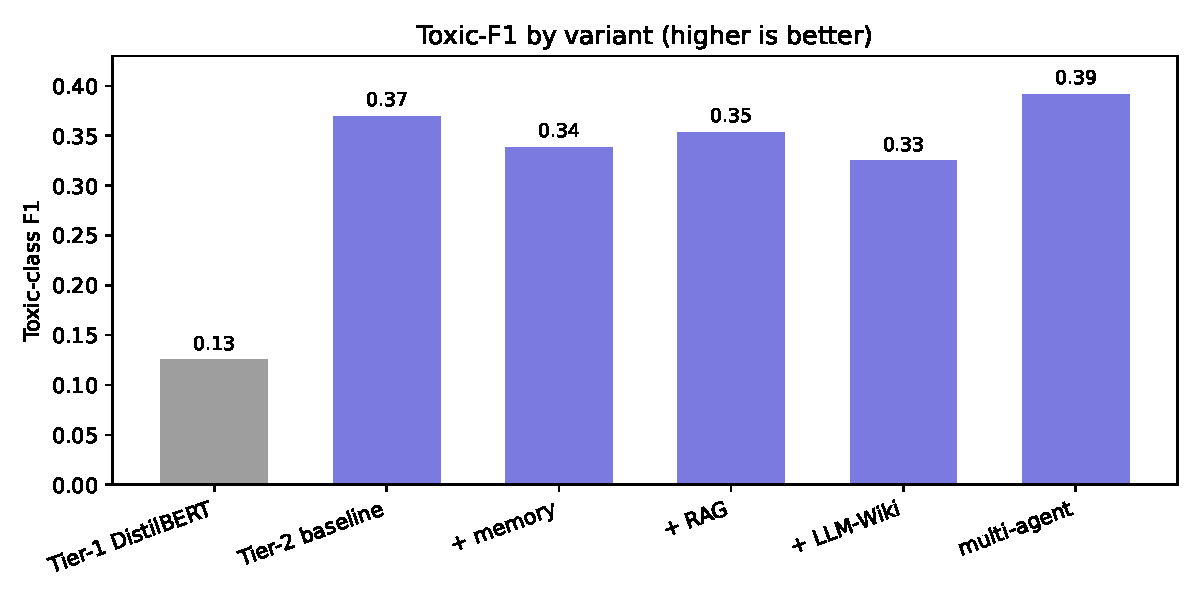
\includegraphics[width=0.9\linewidth,height=0.85\textheight,keepaspectratio]{figures/toxic_f1_by_variant.pdf}
\caption{Toxic-class F1 by variant. The two-tier baseline more than doubles Tier-1, and the multi-agent configuration leads the context variants.}\label{fig:toxicf1}
\end{figure}

\section{Reading the results}\label{reading-the-results}

\textbf{Tier-1 alone is a poor judge, and that is the point.} Its toxic F1 is 0.13 and its precision 0.07. Put plainly: when the static model shouts ``toxic,'' it is wrong roughly fourteen times out of fifteen. This is not a flaw. It is why the model sits first and not last, being fast, blind, good for surfacing suspects and useless as the final word. Those false alarms are exactly what the second tier is there to clean up.

\textbf{The two-tier design keeps its main promise.} Adding the LLM judge lifts toxic F1 from 0.13 to 0.37 and precision from 0.07 to 0.27. Behind the numbers, the judge is catching the static model's over-flagging: messages that look toxic to a word-counting model but read as ordinary in context, gaming trash talk, an angry but fair product review, get corrected. This answers RQ2, and it is the biggest effect in the study.

\textbf{Memory and RAG barely move the needle.} Memory nudges F1 down slightly, 0.37 to 0.34, and RAG down a touch to 0.35. Both stay next to the baseline. Knowing an author's recent history or seeing a handful of similar past cases simply did not change many verdicts here.

Section~\ref{why-memory-and-rag-stayed-neutral} goes into why this is happening, but the short answer is about the data and it can be quantified. The 1,748 messages come from 1,364 distinct authors. Of those, 1,134, or 83.1 per cent, appear exactly once, and the median author contributes a single message. A memory module asked to profile an author from one prior line has almost nothing to work with, and the same thinness limits the pool of past cases RAG can draw a close precedent from.

That is a limit of the data, not a mark against the context research. The most toxic content is deleted by moderators and automated filters before anyone can collect it, so the benchmark holds only eighty toxic messages, and the very cases these modules are built for are rare by nature. On a score driven by those eighty, a real gain on the normal majority hardly shows at all.

\textbf{The gap here is scarcity, not the modules themselves.} Splitting the set by collection order gives a partial check on that claim. Table~\ref{tab:scaling-toxic} scores the same variants first on the early subset, which held forty-four toxic messages, and then on the full eighty. Every configuration scores higher once the extra toxic examples arrive. The ordering stays inside the noise, and no context module overtakes the plain baseline at either size, so the headline conclusion is unchanged. But the direction is telling: as the toxic class grows, scores go up, not down. That is what a starved metric looks like, not a broken module, and it is the concrete reason the future-work chapter calls for growing the toxic class.

\begin{longtable}{@{}lll@{}}
\caption{Toxic-class F1 as the toxic set grows from 44 to 80 messages.}\label{tab:scaling-toxic}\tabularnewline
\toprule
Variant & F1 (44 toxic) & F1 (80 toxic) \\
\midrule
\endfirsthead
\toprule
Variant & F1 (44 toxic) & F1 (80 toxic) \\
\midrule
\endhead
\bottomrule
\endlastfoot
Tier-1 & 0.10 & 0.13 \\
Tier-2 baseline & 0.29 & 0.37 \\
Tier-2 + memory & 0.33 & 0.34 \\
Tier-2 + RAG & 0.27 & 0.35 \\
Tier-2 + LLM-Wiki & 0.28 & 0.33 \\
Tier-2 multi-agent & 0.35 & 0.39 \\
\end{longtable}

\textbf{The LLM-Wiki trades precision for recall, and loses the trade.} It matches the baseline on recall at 0.57, tied for the highest in the table, then drops to the lowest precision of any Tier-2 variant, 0.23, for an F1 of 0.33. The curated policy and glossary make the judge more suspicious. It catches as much toxicity as anything else and flags more innocent messages doing it, behaving rather like a moderator who has just read the rulebook cover to cover and now sees a violation everywhere.

\textbf{The multi-agent setup wins, and it wins by being careful rather than eager.} Its F1 of 0.39 is the best in the table. The shape of that win matters, though. It comes from the highest precision, 0.33, not the highest recall; its recall of 0.47 is in fact the lowest of the group. Splitting the decision across a risk scorer, a profiler, an escalator, and a supervisor produces a more cautious judge. It flags less. When it does flag, it is right more often.

\begin{figure}[H]
\centering
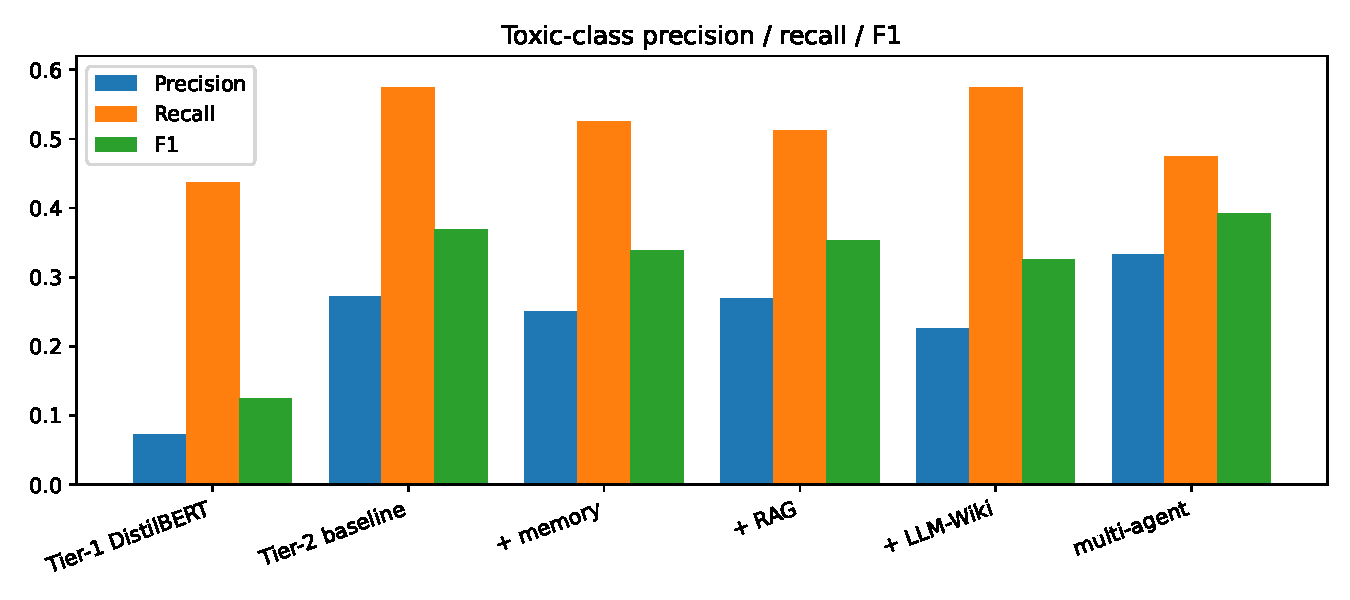
\includegraphics[width=0.9\linewidth,height=0.85\textheight,keepaspectratio]{figures/toxic_prf_by_variant.pdf}
\caption{Toxic-class precision, recall, and F1 side by side, showing the precision-recall trade-off each variant strikes.}\label{fig:toxicprf}
\end{figure}

\section{Inside the multi-agent chain}\label{inside-the-multi-agent-chain}

Each specialist writes its own signal to the record, so the winning variant can be opened up instead of treated as a black box. Doing that explains both what it achieved and what it did not. Table~\ref{tab:routing} gives the escalation router's decisions across the benchmark.

\begin{longtable}{@{}lll@{}}
\caption{Routing decisions made by the escalation agent (n = 1,748).}\label{tab:routing}\tabularnewline
\toprule
Action & Messages & Share \\
\midrule
\endfirsthead
\toprule
Action & Messages & Share \\
\midrule
\endhead
\bottomrule
\endlastfoot
Cleared automatically & 1,647 & 94.2\% \\
Flagged automatically & 57 & 3.3\% \\
Sent to human review & 44 & 2.5\% \\
\end{longtable}

Two things follow from that table.

First, the escalation path is live rather than ornamental. The router sent 44 messages to a person, flagged 57 on its own, and cleared the rest, which shows the three available actions are genuinely told apart instead of collapsing onto one default. The seam the design reserves for a human is therefore reached in practice, not merely declared. What it does not settle is the staffing question, and the gap between the two is wider than the figure suggests. One in forty is the rate inside the benchmark, and the benchmark is not ordinary traffic. Chaining the measured rates together gives a rough sense of the live equivalent: about eight per cent of messages reach the second tier at all, and about two and a half per cent of those are routed onward, which puts human review closer to one message in four hundred. Even that is an estimate rather than a measurement, and a generous one, since the benchmark's low-confidence portion is itself weighted towards difficult cases and will overstate how often the router reaches for a person. Whether any such load is workable then depends on arrival rate, on how long a reviewer needs per case, and on how many reviewers there are, none of which this study measures. The number shows the mechanism functions. Sizing it for a real moderation team is a separate exercise.

Second, and more interesting: the behaviour profiler returned low risk on \emph{every one} of the 1,748 records, covering 1,364 distinct authors. Not one came back medium or high. This is not a parse failure, since the chain falls back to ``medium'' when a response cannot be read. It is the profiler doing its job on data that gives it nothing. With 83.1 per cent of authors appearing exactly once, there is no pattern of prior behaviour to find, so the profiler correctly reports the absence of one, and the agent meant to contribute author history contributes a constant instead.

That sharpens how the multi-agent win should be read. The gain in precision cannot be coming from behavioural profiling, because that signal never varied at all. It comes from what is left: a risk score computed on content alone, a routing decision, and a supervisor forced to reconcile them. The same data sparsity that flattened memory and RAG also silenced one of the four agents, and the decomposition still won. Which suggests the benefit lies in splitting the judgement itself, rather than in any extra information the individual steps were supposed to supply.

\section{Confusion matrices}\label{confusion-matrices}

The confusion matrices in Figure~\ref{fig:confusion} show where the errors fall, not just how many there are. They tell the same story as the F1 column in a more concrete form. Tier-1's matrix is full of false positives in the top-right cell. The two-tier baseline shrinks that cell sharply. The Wiki variant lets it grow again as it over-flags. And the multi-agent matrix has the smallest false-positive cell of all, while still keeping a competitive count of true positives.

\begin{figure}[H]
\centering
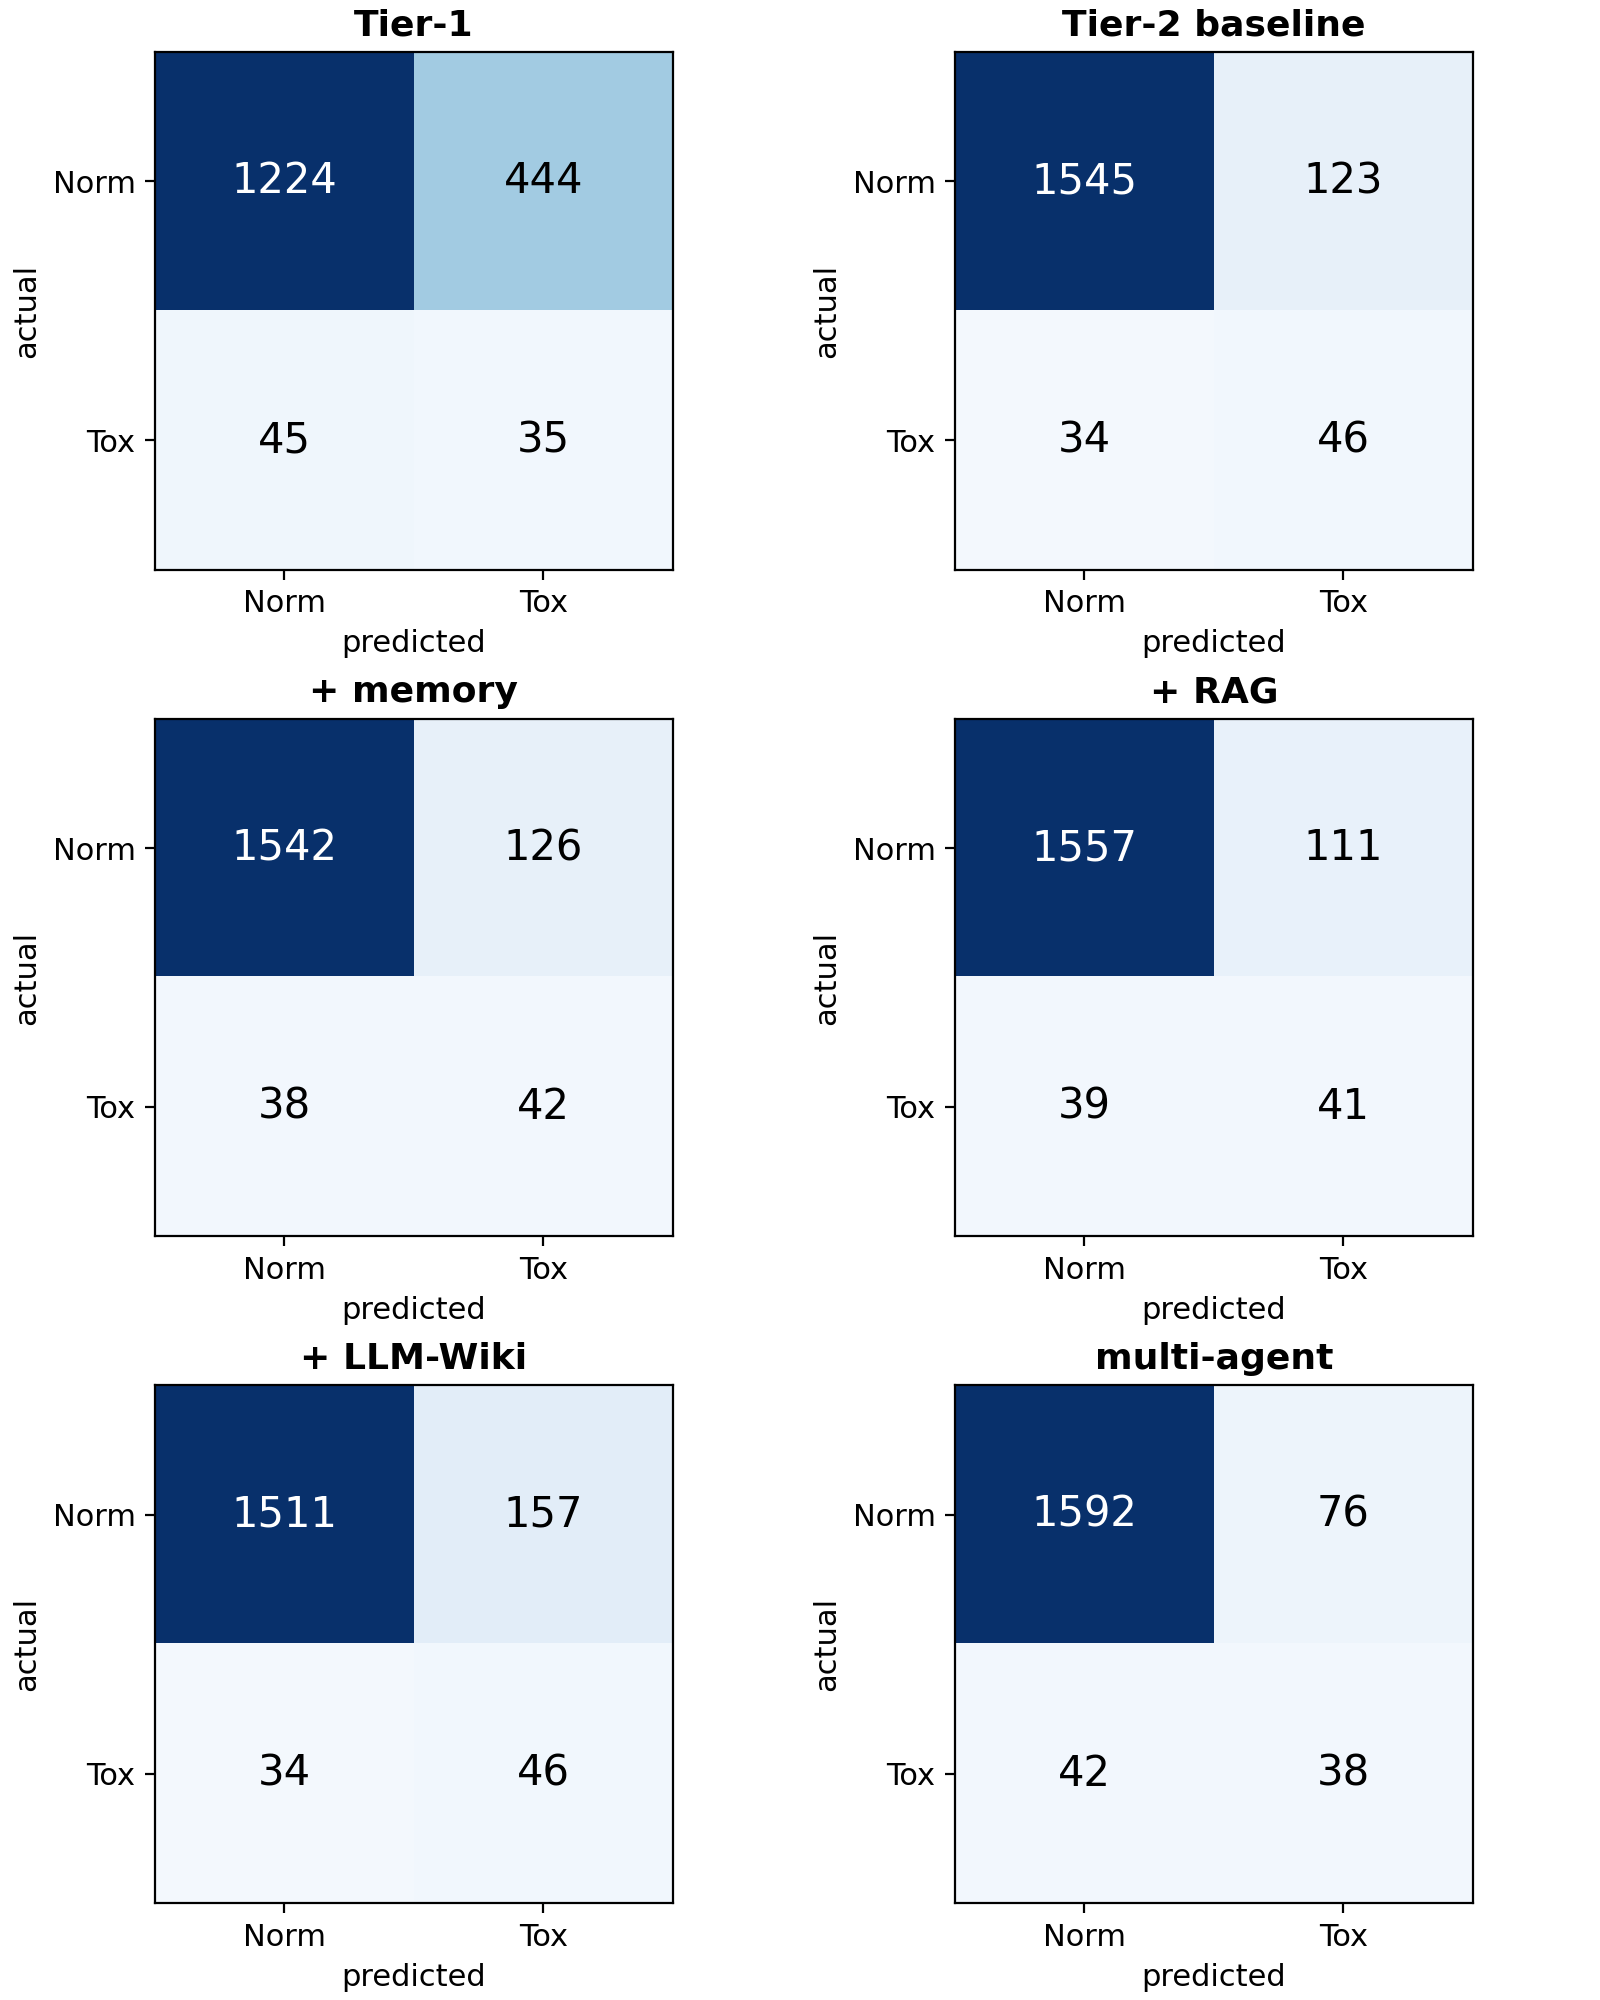
\includegraphics[width=0.9\linewidth,height=0.85\textheight,keepaspectratio]{figures/confusion_matrices_by_variant.png}
\caption{Binary confusion matrices per variant.}\label{fig:confusion}
\end{figure}

\section{Statistical significance}\label{statistical-significance}

With only 80 toxic messages, a handful of verdicts can swing an F1 score. So the real question is whether the gaps in Table~\ref{tab:headline} are solid. McNemar's test answers it by looking only at the messages where two systems disagree, then asking whether a variant fixes more of the baseline's mistakes than it creates. Table~\ref{tab:mcnemar} sets each variant against the Tier-2 baseline.

\begin{longtable}{@{}
  >{\raggedright\arraybackslash}p{\dimexpr 0.2000\linewidth - 1.60\tabcolsep \relax}
  >{\raggedright\arraybackslash}p{\dimexpr 0.2000\linewidth - 1.60\tabcolsep \relax}
  >{\raggedright\arraybackslash}p{\dimexpr 0.2000\linewidth - 1.60\tabcolsep \relax}
  >{\raggedright\arraybackslash}p{\dimexpr 0.2000\linewidth - 1.60\tabcolsep \relax}
  >{\raggedright\arraybackslash}p{\dimexpr 0.2000\linewidth - 1.60\tabcolsep \relax}@{}}
\caption{McNemar's test vs the Tier-2 baseline (toxic-vs-normal correctness).}\label{tab:mcnemar}\tabularnewline
\toprule
Variant & Baseline right, variant wrong & Variant right, baseline wrong & p-value & Verdict \\
\midrule
\endfirsthead
\toprule
Variant & Baseline right, variant wrong & Variant right, baseline wrong & p-value & Verdict \\
\midrule
\endhead
\bottomrule
\endlastfoot
+ memory & 63 & 56 & 0.582 & not significant \\
+ RAG & 52 & 59 & 0.569 & not significant \\
+ LLM-Wiki & 85 & 51 & \textbf{0.005} & significant, favours \textbf{baseline} \\
\textbf{multi-agent} & 40 & 79 & \textbf{\textless{} 0.001} & significant, favours \textbf{multi-agent} \\
\end{longtable}

Two results are significant, and they point in opposite directions.

The multi-agent system fixes 79 messages the baseline got wrong and breaks only 40. A genuine gain, not luck. The LLM-Wiki does the reverse: it changes many verdicts, 136 in all, more than any other variant, but the baseline is right on 85 of them against the Wiki's 51, so its over-flagging is a real effect rather than noise. Memory and RAG land in the middle, each disagreeing with the baseline about as often as it agrees, neither difference significant. Which is the statistical way of saying they neither helped nor hurt here.

\section{RAG versus the LLM-Wiki}\label{rag-versus-the-llm-wiki}

This is the head-to-head the two retrieval backends were built for.

On F1, vector RAG at 0.35 just edges out the curated-knowledge Wiki at 0.33, and they get there differently. RAG keeps the baseline's precision of 0.27 and trims recall. The Wiki keeps the baseline's recall and drops precision. Put simply: past cases nudged the judge toward caution, curated knowledge nudged it toward suspicion. Neither beat the plain baseline on this set, but the Wiki's effect was the larger of the two, and by Table~\ref{tab:mcnemar} the only significant one. Chapter 6 picks up what that says about the two ways of grounding a judge.

\begin{figure}[H]
\centering
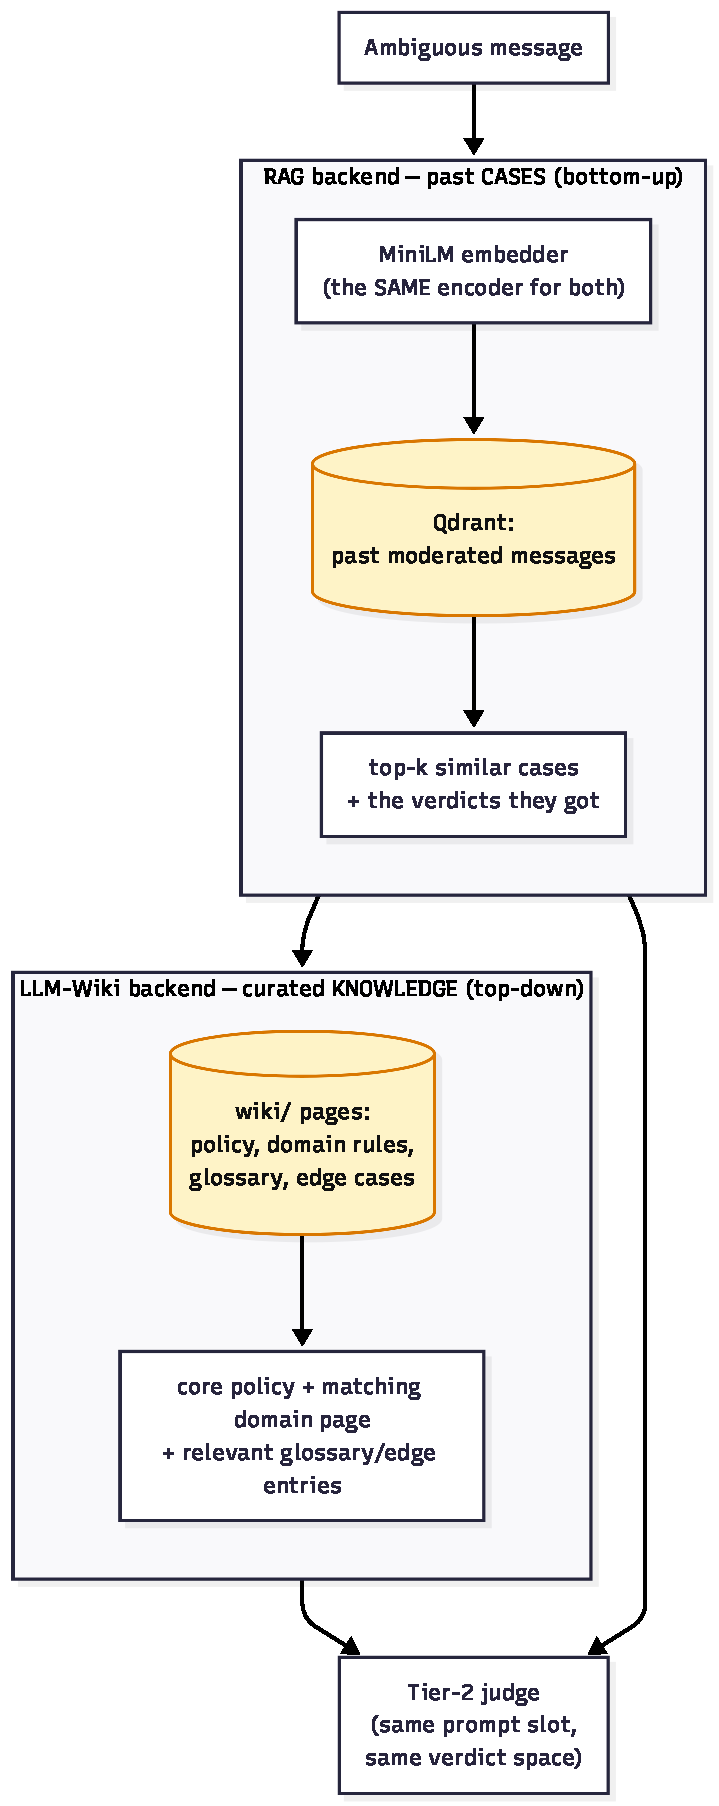
\includegraphics[width=0.9\linewidth,height=0.85\textheight,keepaspectratio]{figures/rag_vs_wiki.pdf}
\caption{RAG versus the LLM-Wiki: the two backends share the same embedder but draw on different corpora, RAG on past cases and the Wiki on curated knowledge, feeding the same judge in the same verdict space.}\label{fig:ragwiki}
\end{figure}

\section{Latency and computational cost}\label{latency-and-computational-cost}

Accuracy is only half the picture. What each verdict costs is the other half, and it is where the two tiers split most sharply. Table~\ref{tab:latency} has the timings.

\begin{longtable}{@{}lllll@{}}
\caption{Per-message latency for the two tiers.}\label{tab:latency}\tabularnewline
\toprule
Stage & Mean & Median & 95th pct & 99th pct \\
\midrule
\endfirsthead
\toprule
Stage & Mean & Median & 95th pct & 99th pct \\
\midrule
\endhead
\bottomrule
\endlastfoot
Tier-1 (DistilBERT) & 31 ms & 28 ms & 49 ms & 86 ms \\
Tier-2 (LLM judge) & 5.3 s & 4.6 s & 9.1 s & 12.8 s \\
\end{longtable}

Tier-1 labels a message in about 31 milliseconds. A single Tier-2 judgement takes about 5.3 seconds. That is a 174-fold gap, and it is the whole reason the second tier is used sparingly: running a five-second model on every message of a live stream is not an option, so it is saved for the low-confidence minority and run off the live path where it does not slow the stream.

The context modules add to that Tier-2 cost by different amounts, which matters when reading Table~\ref{tab:headline}. Memory adds a quick history lookup. RAG and the Wiki each add an embedding step and a search. The multi-agent setup makes four LLM calls instead of one, so it costs about four times the baseline judge, roughly twenty seconds a message. Table~\ref{tab:cost} puts cost next to benefit.

\begin{longtable}{@{}llll@{}}
\caption{Computational cost per message, by stage and variant.}\label{tab:cost}\tabularnewline
\toprule
Stage / variant & LLM calls & Typical latency & Toxic F1 \\
\midrule
\endfirsthead
\toprule
Stage / variant & LLM calls & Typical latency & Toxic F1 \\
\midrule
\endhead
\bottomrule
\endlastfoot
Tier-1 DistilBERT & 0 & 31 ms & 0.13 \\
Tier-2 baseline & 1 & 5.3 s & 0.37 \\
Tier-2 + memory & 1 (+ history fetch) & 5.3 s & 0.34 \\
Tier-2 + RAG & 1 (+ embed + search) & 5.5 s & 0.35 \\
Tier-2 + LLM-Wiki & 1 (+ embed + lookup) & 5.5 s & 0.33 \\
Tier-2 multi-agent & 4 & 21 s & \textbf{0.39} \\
\end{longtable}

Read together, that table changes how the multi-agent result looks. Its win on F1 is real and significant, and it comes at four times the cost of a single-shot judge. Any real deployment would have to decide whether the extra accuracy is worth the extra spend. The discussion of limits returns to this.

\section{Throughput, scalability, and resource use}\label{throughput-scalability}

Before the numbers, a word on how they were obtained, since a performance claim is only as good as its protocol. The latency figures in Table~\ref{tab:latency} are not estimates: the pipeline records the wall-clock time of every Tier-1 inference and every Tier-2 judgement as a field on the stored record, so the percentiles are computed over all 1,748 benchmark messages rather than sampled. Throughput was measured separately, by running the same fine-tuned classifier over messages drawn from the collected stream log in a loop, with a warm-up pass excluded and model loading timed apart from inference, and with Kafka and Elasticsearch out of the path so the figure reflects the model rather than the plumbing. Resource use was sampled once every two seconds during a sustained run, from the operating system and from the container runtime. All three are driven by scripts kept in the repository, so a reader can reproduce them on their own hardware and get a comparable set of numbers.

Latency is how long one message takes. Throughput is how many the pipeline handles per second, and it is the figure that decides whether the system can keep up with a live stream. Measured this way, Tier-1 handles about \textbf{thirty messages a second} on the single laptop used throughout, with full specifications in Appendix B. That is roughly 1,800 a minute, all on CPU. A busy live chat rarely runs past a few messages a second, so one machine has plenty of room to spare.

The raw rate matters, but so does whether it grows when compute is added. Table~\ref{tab:scaling} shows what happens as classifier processes are added, each pinned to one core. Throughput climbs, but by less each time, because one process already spreads across the laptop's four cores and they fill up fast. The real point is the direction, not the ceiling: adding compute adds throughput.

Two things should be said plainly about how far that extends. The deployment measured here runs Kafka with a single partition, so in the live pipeline exactly one Tier-1 consumer draws from the stream at a time; the numbers in Table~\ref{tab:scaling} come from running the classifier itself in parallel, which measures the compute tier rather than the full ingest path. Growing beyond one node therefore means raising the partition count first, after which consumers can be added on the same machine or on others with no change to producers, schema, or downstream code. That step is a configuration change, not a redesign, but it was not needed here and so was not measured. One node is capped by its cores; the architecture is not, and the distinction between what was measured and what follows from the design is drawn deliberately.

\begin{longtable}{@{}ll@{}}
\caption{Tier-1 throughput as CPU cores are added.}\label{tab:scaling}\tabularnewline
\toprule
Classifier processes & Throughput \\
\midrule
\endfirsthead
\toprule
Classifier processes & Throughput \\
\midrule
\endhead
\bottomrule
\endlastfoot
1 core & 17 msg/s \\
2 cores & 22 msg/s \\
4 cores & 25 msg/s \\
All cores, single process & 30 msg/s \\
\end{longtable}

Resource use under a steady load shows where the cost sits. Table~\ref{tab:resource} has the figures. Driving the classifier flat out pushes the CPU to its limit while the GPU stays almost idle, which confirms Tier-1 is CPU-bound, as expected for a small model run without GPU offload, and that the graphics card is not the bottleneck. Memory is the tighter limit on this machine. The containers themselves are cheap: Qdrant, Spark, Kafka, and Elasticsearch together use a fraction of a core and a few hundred megabytes while Tier-1 runs, because the heavy work is the model, not the plumbing.

\begin{longtable}{@{}ll@{}}
\caption{Resource use while Tier-1 runs under sustained load.}\label{tab:resource}\tabularnewline
\toprule
Component & Use under load \\
\midrule
\endfirsthead
\toprule
Component & Use under load \\
\midrule
\endhead
\bottomrule
\endlastfoot
Host CPU & 100\% peak, 88\% average \\
GPU & about 300 MB, under 10\% \\
Host memory & about 94\% \\
Containers (Kafka, Spark, Elasticsearch, Qdrant) & under 1\% CPU, a few hundred MB total \\
\end{longtable}

Put next to the latency figures, these answer RQ1 directly. The pipeline labels live messages from more than one platform at a median of 28 milliseconds and a steady thirty a second, on one modest laptop. For the target setting, that is real-time.

One distinction matters here more than anything else in the section, because only half of it has been tested. That throughput grows as cores are added is a measured result, and Table~\ref{tab:scaling} is the evidence for it. That the same would hold across separate machines is not. It follows from the architecture, since a partitioned log feeding stateless consumers is built to spread precisely that way, but a design supporting something and a thesis demonstrating it are different claims. Multi-node scaling is therefore recorded here as a capability the architecture provides and a validation still outstanding, not as a finding. Running that cluster benchmark is the obvious next step, and it belongs to future work rather than to this evaluation.

\section{Answering the research questions}\label{rq-summary}

The evidence in this chapter lines up with the three research questions, one row each. The design that motivated the study, from Chapters 3 and 4, fills the left of each row; this chapter fills the right. The path from question to answer can be followed straight across. Table~\ref{tab:rq} lays it out.

\renewcommand{\arraystretch}{1.5} 

\begin{longtable}{@{}
  >{\raggedright\arraybackslash}p{\dimexpr 0.07\linewidth - 1.6\tabcolsep \relax}
  >{\raggedright\arraybackslash}p{\dimexpr 0.25\linewidth - 1.6\tabcolsep \relax}
  >{\raggedright\arraybackslash}p{\dimexpr 0.22\linewidth - 1.6\tabcolsep \relax}
  >{\raggedright\arraybackslash}p{\dimexpr 0.26\linewidth - 1.6\tabcolsep \relax}
  >{\raggedright\arraybackslash}p{\dimexpr 0.20\linewidth - 1.6\tabcolsep \relax}@{}}
\caption{Each research question traced from design choice to experiment, evidence, and answer.}\label{tab:rq}\tabularnewline
\toprule
\textbf{RQ} & \textbf{Design choice} & \textbf{Experiment (metric)} & \textbf{Evidence} & \textbf{Answer} \\
\midrule
\endfirsthead
\toprule
\textbf{RQ} & \textbf{Design choice} & \textbf{Experiment (metric)} & \textbf{Evidence} & \textbf{Answer} \\
\midrule
\endhead
\bottomrule
\endlastfoot

\textbf{RQ1} & Partitioned Kafka log, decoupled tiers, per-platform adapters & Latency, throughput, scaling, resources (Sections~\ref{latency-and-computational-cost} and~\ref{throughput-scalability}) & 28 ms median, about 30 msg/s, rises with cores; two platforms, eleven domains & \textbf{Yes.} Real-time, multi-platform, easy to extend \\
\addlinespace[1em]

\textbf{RQ2} & Fast DistilBERT with a 0.80 confidence gate and a selective LLM auditor & Tier-1 vs Tier-2 baseline (Table~\ref{tab:headline}) & Toxic F1 from 0.13 to 0.37, precision from 0.07 to 0.27 & \textbf{Yes.} The study's largest effect \\
\addlinespace[1em]

\textbf{RQ3} & Temporal memory, RAG/Wiki, and multi-agent as switchable modules & Per-variant F1 and McNemar's test (Tables~\ref{tab:headline} and~\ref{tab:mcnemar}) & Multi-agent 0.39 (p \textless{} 0.001); memory and RAG not significant; Wiki significantly worse & \textbf{Partly.} Only the multi-agent decomposition helps \\

\end{longtable}
% Reset arraystretch to default for the rest of the document
\renewcommand{\arraystretch}{1.0}

RQ3 is the one qualified answer, and the qualification is the finding itself. Added context helps when it gives the decision structure, as the agent breakdown does. It does not help when it merely hands more information to a single judge.

\chapter{Discussion}\label{discussion}

The results in Chapter~\ref{evaluation-and-results} are more interesting for their shape than their size. The headline is not that one configuration scored highest. It is that four ways of adding context behaved so differently from one another, and that the only two significant effects point in opposite directions. This chapter works through why.

\section{Context helps, but only the right kind}\label{context-helps-but-only-the-right-kind}

A flat assumption sits behind a great deal of ``add more context'' engineering: that more information can only help. These results push back on it.

Two of the four modules, memory and RAG, left the score essentially unchanged. A third, the LLM-Wiki, made it significantly worse. Only the multi-agent chain produced a significant gain, and that gain is in overall correctness: it removes false alarms rather than catching more toxicity. So whatever ``context helps'' means here, it is clearly conditional, and the condition has less to do with how much context is added than with how that context is structured and used.

\section{The central tension: precision against recall}\label{the-central-tension-precision-against-recall}

Almost everything in Chapter~\ref{evaluation-and-results} is a story about one trade-off.

Toxic messages are rare, so every system is walking a tightrope. Lean towards flagging and it catches more toxicity but also more innocents: recall up, precision down. Lean towards restraint and it makes fewer false accusations but misses more: precision up, recall down. It is the tension a smoke alarm faces. Too sensitive and it goes off whenever someone makes toast, so people stop trusting it. Too dull and it stays silent during a real fire. F1 is just a way of scoring how well a system balances the two.

Seen through that lens the variants line up cleanly. The baseline sits in the middle. The Wiki turns the sensitivity up, holding recall and losing precision, the alarm that cries toast. The multi-agent chain turns it down. It does give up some toxicity, eight fewer toxic messages caught than the baseline, but it removes far more false alarms, 47 fewer, which is why it is the only one whose balance actually improves.

\section{Why memory and RAG stayed neutral}\label{why-memory-and-rag-stayed-neutral}

The likeliest explanation is not that the ideas are wrong but that the data starves them.

Both depend on there being something to retrieve. Memory needs an author to have a history. RAG needs the message to have close neighbours among past cases. On this benchmark, gathered in a single day from many short-lived live sessions, most authors appear only once, and author history reached the judge for fewer than one message in ten (Section~\ref{reading-the-results}), so the ``history'' the memory module works with is usually empty. A profile built on one prior message is barely a profile. RAG hits a softer version of the same wall: with a modest precedent pool, the nearest past case is frequently not very near, and a weak analogy is easy for the judge to ignore. Pavlopoulos and colleagues met the same wall from the other side: context changed how people labelled comments, yet making classifiers context-aware brought no measurable gain, and they too concluded that larger datasets annotated in context were needed \citep{pavlopoulos2020context}.

This reading has a testable consequence, which matters for a thesis. Both modules should come alive on data where authors recur and the precedent pool is dense. This benchmark does not offer that kind of data, and collecting it is left to future work (Section~\ref{future-work}). It is also the reason to report these two as \emph{neutral on this benchmark} rather than as failures.

\section{Why the curated knowledge over-flags}\label{why-the-curated-knowledge-over-flags}

The Wiki result is the most instructive of the four, because it fails legibly.

Feeding the judge a policy page, a dog-whistle glossary, and a list of edge cases made it more suspicious, and the suspicion was indiscriminate: recall held steady while precision fell. The knowledge base is, in effect, a briefing on everything that can go wrong, and a judge who has just read it starts seeing hazards everywhere, much the way a first-aid course can leave someone convinced every headache is serious.

That diagnosis points at the fix rather than away from it. The starter knowledge base is broad and blunt. It names categories of harm without the precise boundaries that stop a rule from over-firing. A glossary entry saying ``watch for coded replacement rhetoric'' could flag any mention of immigration; the same entry, scoped with counter-examples, would not. So the low precision is a property of a small, early knowledge base, not of the curated-knowledge idea itself.

It also sharpens the contrast this thesis set out to draw. On this benchmark, retrieving past \emph{cases} disturbed the baseline less than injecting general \emph{rules}, plausibly because a specific precedent is self-limiting in a way a general rule is not. Whether a carefully scoped knowledge base closes that gap is the natural next experiment, and a graph-structured version, GraphRAG, is one route to the precision a flat base lacks.

\section{What the multi-agent win actually shows}\label{what-the-multi-agent-win-actually-shows}

The multi-agent chain is the one significant success, and it is worth being precise about why, because the obvious explanation is not quite right.

It did not win by being smarter about toxicity in general. Its recall is the lowest of the Tier-2 variants. It won by being disciplined. Splitting the judgement into a risk score, a behaviour profile, a routing decision, and a final reconciliation forces the model to separate ``is this content risky'' from ``what should happen next'', and a verdict that has to survive several steps is harder to reach carelessly. The chain also asks ``is this author risky'', but on this benchmark that step contributed nothing, since the Behaviour Profiler rated every author low risk (Section~\ref{inside-the-multi-agent-chain}), so the gain has to come from the other three. On this reading the gain is not extra knowledge but reduced impulsiveness, which fits the fact that it shows up as higher precision. A committee tends to overturn fewer sound decisions than a single hurried reviewer for a similar reason: the friction is the feature.

\section{How the judge fails}\label{how-the-judge-fails}

The judge is not infallible, and its mistakes are as informative as its successes. Its errors lean towards leniency. The baseline judge misses 34 of the 80 toxic messages, 43 per cent, while wrongly flagging 123 of the 1,668 normal ones, 7 per cent. The internship phase of this work studied such misses closely and traced them to one root cause, which it named \emph{implicit-bias blindness}, with three patterns recurring inside it. The first can be checked on this benchmark; the other two come from that earlier error analysis.

The first is over-correction in permissive domains. In a stream tagged low-strictness, gaming for instance, the judge learns that aggression is usually just trash talk, then carries that expectation too far and waves through almost all hostile language as banter. A reasonable assumption hardening into a blind spot, the way a lifeguard who has seen a hundred false alarms grows slow to the hundred-and-first. The benchmark bears this out: in gaming streams the judge caught only 2 of the 14 toxic messages, and across low-strictness streams it missed 19 of 36, against 10 of 35 in high-strictness ones.

The second is veiled sarcasm and semantic drift. The judge reads a literal message well. A sentence whose harm lives in its tone, or in a meaning that has drifted from the plain words, slips past. A polite surface wrapped around hostile intent is exactly what a single-shot reading handles worst.

The third is the hardest: the niche dogwhistle. Some coded language cannot be resolved from one message at all. Deciding whether a phrase is innocent or an attack requires knowing that this particular user has used it as an attack before. That is not a gap the judge can close on its own, and it is the strongest argument in the whole thesis for the mechanisms that reach outside the single message, temporal memory and, in the last resort, a human. The internship system made that last resort explicit as a Targeted Behavioural Review tool, letting a human moderator pull a user's full history and rule on the pattern rather than the line. The lesson carries into this work unchanged: automated layers clear the high-volume noise, and the deepest, most context-dependent cases still land on a person's desk, by design rather than by failure.

\section{The human role these results actually show}\label{the-human-role}

It would be easy to read Chapter~\ref{evaluation-and-results} as a comparison of six automated configurations. That reading misses the fact that people are present at three separate points in this study, and that one of them, although never measured, may have shaped the results more than any configuration did.

The first is annotation. Every score in this thesis is a measurement against 1,748 messages read and labelled by hand. No model in the comparison ever encounters ground truth; it encounters one person's judgement about what a message meant in the place it appeared, and the entire evaluation is an account of how closely each configuration reproduces those judgements. That labour is the foundation the other two chapters stand on, and it is worth naming rather than treating as a preprocessing step.

The second is escalation. The multi-agent chain routed 44 messages to human review and cleared 94.2 per cent automatically, which puts the human-in-the-loop idea this thesis borrows from Crossmod and Automoderator \citep{chandrasekharan2019crossmod, jhaver2019automod} into concrete form: the machine takes the volume and a person is called for a minority of cases. What that minority would amount to in a working deployment is not something this study can answer, since it depends on arrival rate and reviewer capacity rather than on the share alone. The direction still matters, though. A system referring a quarter of its traffic to a moderator would be unusable, and one referring nothing would be the unaccountable automation the literature warns against \citep{gillespie2018custodians}. What the results establish is that the route exists and is taken, which is the precondition for tuning it.

The third was never measured directly: the human moderators working upstream, on the platforms the data came from. The likeliest reason the toxic class stayed at eighty messages, set out in Section~\ref{limitations}, is that moderators and their automated tools remove the worst content before an ingestion pipeline can see it.

Read the other way round, the central difficulty of this thesis is consistent with existing human moderation being effective. The scarcity that starved the memory and RAG modules, that left only eighty positives to compute F1 over, and that forced every conclusion about small effects to be hedged, may be the visible shadow of moderators doing their job well. This is worth stating because it cuts against the framing that usually motivates work like this. Automated moderation is not needed because humans are failing; on well-run channels they appear to be succeeding, at a cost in labour and exposure the literature documents carefully \citep{roberts2019behindscreen, wohn2019volunteer}. What automation offers is scale and speed at the moments a small volunteer team cannot cover, which is precisely the division of labour that Section~\ref{context-helps-but-only-the-right-kind} onward has been describing.

\section{Limitations}\label{limitations}

Several limits bound how far these results should be pushed.

\textbf{The toxic class is small.} Eighty toxic messages is enough to detect a strong effect, since the multi-agent chain's gain in overall correctness clears the significance bar comfortably, but not enough to resolve small ones, and its gain in toxic F1 alone stays within the uncertainty. The neutral readings for memory and RAG should be read as ``no detectable effect on this set,'' not ``no effect,'' and the priority for the next round is more labelled toxicity.

\textbf{Collecting toxic data is harder than it sounds.} A practical obstacle shaped the whole dataset. On well-run channels, automated filters hold the most toxic messages back for review, and a short chat delay lets moderators remove others before they appear \citep{youtubelivechat2026, twitchapi2026}, so much of that content never reaches a pipeline that reads chat as a viewer does. The system is, in effect, trying to study a phenomenon the environment is actively erasing, and that is the deeper reason the toxic class stayed small however long collection ran. The lesson for future data work is to sample from lightly-moderated or unmoderated spaces, where toxic content survives long enough to be recorded, rather than from the very platforms whose job is to remove it.

\textbf{A single annotator.} The ground truth was labelled by one reviewer, so it carries one person's reading of the borderline cases, and hate-speech judgements are known to vary between annotators \citep{ross2017reliability, disagreerationales2026}. A second labeller on a subset, with an agreement score, would firm up the foundation the whole comparison rests on.

\textbf{Latency and cost.} Every gain from the second tier is bought with LLM calls that take seconds, and the multi-agent variant spends four of them per message. The tiered design keeps that off the live path, but the cost is real and would shape any production deployment.

\textbf{Scope.} The benchmark is English-language, text-only, and drawn from two platforms, YouTube and Twitch, both of them live-chat sources. Two further sources were considered and set aside: Reddit, whose API grants script credentials only to an established account, and Trustpilot, which refuses automated collection. Both are access restrictions rather than design limits, but the effect on this study is the same, and nothing here shows how the findings travel to threaded discussion or to long-form review text. Nor does anything here speak to images, audio, other languages, or the coordinated behaviour that plays out across many messages rather than within one.

\textbf{Screen blindness.} The judge reads a stream's domain from its metadata, but it never sees the live audio or video, and that gap has real consequences. A broadcast whose topic shifts halfway through keeps a context tag that has quietly gone stale. A joking or misleading stream title sends the Context Agent down the wrong path from the very first message. And any harm living in what is shown or said aloud, rather than typed, is simply invisible to the system. The pipeline reasons about text in a world that is audiovisual, and wherever the two diverge, it is guessing. Closing that gap means giving the context layer access to more of the stream than its title, which is a direction rather than a fix.

\chapter{Conclusion and Future Work}\label{conclusion-and-future-work}

This thesis set out to build a moderation pipeline that could be fast and context-aware at once, then to measure honestly how much each kind of added context was really worth. This closing chapter states what was achieved against the research questions, addresses the ethical questions the system raises, and lays out the work that follows from it.

\section{Summary}\label{summary}

What was delivered is a modular, real-time Big Data pipeline for hate-speech detection.

A containerised stack of Kafka, Spark, Elasticsearch, and Qdrant carries messages from more than one platform through a single schema. A fast DistilBERT tier labels every one of them in tens of milliseconds. An asynchronous LLM judge then reviews only the uncertain minority, grounded, at the operator's choice, in temporal memory, retrieved precedents, or a curated knowledge base, or decomposed across four specialist agents. Every one of those configurations was evaluated against a hand-labelled benchmark using imbalance-aware metrics and significance testing, and the whole pipeline was left reproducible from a single command.

\section{Answers to the research questions}\label{answers-to-the-research-questions}

\textbf{RQ1, the infrastructure, is answered in the affirmative.} The pipeline classifies live messages from YouTube and Twitch through one schema, at a median Tier-1 latency of 28 milliseconds and a sustained rate of about thirty messages a second on a single laptop, and that rate rises as cores are added. It also absorbed new context modules and an entire second retrieval backend during the project without any change to the layers beneath them. The modularity was not a claim made on paper. It was exercised repeatedly.

\textbf{RQ2, the two-tier design, is answered clearly, and it is the study's strongest result.} Decoupling a fast static classifier from a selective LLM auditor more than doubled toxic F1, from 0.13 to 0.37, and lifted precision from 0.07 to 0.27, by cleaning up exactly the domain-specific false positives that static models are known to produce. Large, and unambiguous.

\textbf{RQ3, whether extra context improves detection, is answered with a careful ``it depends,'' and that nuance is itself the finding.} Of the three context strategies, only the multi-agent decomposition produced a statistically significant improvement over the single-shot judge (p \textless{} 0.001). Temporal memory and retrieval-augmented moderation left the score statistically unchanged, most plausibly because the data was too sparse in repeat authors and close precedents to feed them. The curated-knowledge LLM-Wiki changed behaviour significantly, but in the wrong direction, its broad rules pushing the judge to over-flag. So the honest answer is that context helped only where it imposed discipline, as the agent decomposition does, rather than mere suspicion, as the flat knowledge base does, or where it depended on data the benchmark could not yet supply.

\section{Ethical considerations}\label{ethical-considerations}

A system that flags people's speech automatically cannot leave its ethics to the end. Two commitments are built in, a third is a balance rather than a guarantee, and one problem stays open.

Privacy is handled at ingestion. The common schema carries only the message, an identifier, and timing, stripping personally identifying information before anything reaches the LLM, so the reasoning layer never sees more of a person than the decision requires. Human authority is preserved by design: the pipeline flags and explains, the multi-agent escalator routes genuinely uncertain cases to a person, and no automated component is given the last word on a ban.

Fairness is the third commitment, and it cuts both ways. Static classifiers inherit the biases of their training data, and those biases surface most often as false positives against distinct dialects and subcultures, a bag-of-words model reading African-American Vernacular English or gaming slang as aggression. The contextual judge softens that bias directly, overriding the static model's rigid thresholds with reasoning, which is part of why the two-tier design cuts false positives so sharply. But it brings a bias of its own in the opposite direction, the leniency documented in Section~\ref{how-the-judge-fails}. Fairness here is therefore not a solved property. It is a balance struck across two tiers, with a human holding final authority over the decisions that cannot be undone.

The open problem is that ``safe'' is not one thing. What counts as acceptable moderation on a public gaming stream is not what counts in a medical or financial setting, and a pipeline built to be domain-agnostic inherits that variability. The right long-term answer is to make the boundary itself dynamic, letting the context layer inject not just a domain label but the privacy and retention rules that domain demands, so the system's own limits flex with the sensitivity of what it is reading. A direction, not a solved problem, and flagged here as such.

\section{Future work}\label{future-work}

Several lines follow directly from the results.

\textbf{Grow the toxic class.} The most immediate need is more labelled toxicity. Eighty toxic messages resolved the large multi-agent effect but not the small ones. A few hundred would turn the neutral readings for memory and RAG from ``undetectable here'' into a firm answer either way, and it is the cheapest high-value work available.

\textbf{Give memory and RAG the data they need.} Section~\ref{why-memory-and-rag-stayed-neutral} traces their flat results to sparse histories and thin precedents, so the natural test is author-dense data where both have something to work with. A measurement gap, not a design one.

\textbf{Distil the judge back into the classifier.} The Tier-2 judge produces something valuable almost as a by-product: a steadily growing set of messages labelled with context-aware verdicts and written explanations. Those verdicts could be captured as a new, context-aware training set and used to fine-tune Tier-1, a teacher-to-student loop in which the slow contextual model teaches the fast blind one. If it worked, the static tier would inherit some of the judge's sense of context, catch more on its own, and gradually lighten the load on the expensive second tier. Whether that loop actually lifts Tier-1, and by how much, is a clean experiment the pipeline is already positioned to run, since every judged record is stored with its verdict. It also turns the running system into its own source of better training data over time.

\textbf{Ensemble self-labelling by inter-variant vote.} A cheaper route to new data follows from a simple observation: the pipeline already holds several genuinely different views of the same message. The baseline judge reasons from the text alone. The memory variant adds the author's history. RAG adds retrieved precedent, the LLM-Wiki adds curated rules, and the multi-agent chain adds a decomposed decision. Treat each as an independent annotator, combine their verdicts by majority or weighted vote, and silver labels appear automatically, in the same spirit that datasets such as Davidson's \citep{davidson2017} and HateXplain \citep{hatexplain2021} were built from the majority vote of several human coders, but without the human cost. Agreement across variants is a natural confidence signal, and their disagreement is arguably worth more still: those are the genuinely ambiguous cases, and routing them to a human instead of discarding them turns the scheme into the human-in-the-loop labelling loop the earlier chapters argue for. The honest caveat is that these voters are not independent the way separate annotators are, since they share one underlying judge, so a shared bias would be amplified rather than cancelled. A dataset built this way would need validating against a small human-labelled gold set before it could train the next model. Used with that guard, it is a low-cost way to grow exactly the toxic-class data these results were short of.

\textbf{Scope the knowledge base.} The LLM-Wiki over-flags because its rules are broad. Tighter, counter-example-rich entries should recover the precision it currently spends, and a graph-structured retrieval such as GraphRAG is one route to the specificity a flat base lacks. The switchable-backend design means either can be dropped in and measured against the vector RAG already in place.

\textbf{Cross-domain validation.} Extending the evaluation to consumer reviews would test whether the findings hold outside live chat. The Trustpilot adapter was written for exactly this, but the site returned HTTP 403 to automated collection, so a published review dataset is the sensible proxy. The ingestion path is already built to receive it, and the same access obstacle applies to Reddit, whose API requires an established account.

\textbf{Stronger Tier-1 baselines.} DistilBERT was chosen for speed on constrained hardware, but the static tier is a swap-in component. Comparing it against stronger encoders, RoBERTa \citep{roberta2019}, DeBERTa \citep{deberta2021}, the domain-specific HateBERT \citep{hatebert2021}, or a purpose-built safety classifier such as Llama Guard \citep{llamaguard2023}, would show whether a better first pass reduces how often the expensive judge has to be called at all.

\textbf{Beyond text, and beyond moderated data.} Two of the study's own limitations mark the last directions. Giving the context layer access to more of a stream than its title, its audio, its video, its shifting topic, would begin to close the screen-blindness gap. And collecting from lightly-moderated sources, where toxic content is not deleted before it can be seen, would build the denser benchmark the toxic-class results have been waiting for.

\textbf{Validate the scale-out path.} Throughput was shown to grow as cores are added on one machine, but the multi-node case rests on the architecture rather than on measurement. Raising the Kafka partition count and running consumers across separate hosts would test whether the ceiling rises as the design predicts. It is a configuration change rather than a redesign, so the experiment is cheap once a cluster is available, and it would convert the horizontal-scaling claim from a property of the design into a result.

\textbf{Edge-aware optimisation and federated learning.} Quantising the static tier for cheaper edge deployment, and training it in a federated, privacy-preserving way, are natural extensions of this architecture. Both are left here as discussed future work rather than implemented, in keeping with the scope agreed for this thesis.

\section{Closing}\label{closing}

The lasting result of this work is not a single best number. It is a demonstration, tested honestly, that context in moderation is neither free nor uniform.

A two-tier design pays for itself handsomely. A disciplined decomposition of the decision pays for itself more modestly, but really. And simply pouring in more information, whether an author's thin history or a broad book of rules, can leave a system no better off or actively worse. For a field that tends to assume more context is always an improvement, that is the finding worth carrying forward.


\appendix
\chapter{Prompt Library}\label{prompt-library}

Every prompt the system sends to an LLM is collected in a single module (\texttt{src/shared\_utils/prompts.py}) rather than scattered through the agents, so the whole prompting strategy can be read, cited, and reused in one place. All calls run at temperature 0 (deterministic, classifier-like behaviour) and force a JSON response, with one automatic retry if the model returns unparseable output. In the templates below, \texttt{\{placeholder\}} marks a value substituted at call time.

\section{Context Agent}\label{context-agent}

Discovers the domain and moderation strictness of a stream from its metadata. The model is \emph{not} shown a fixed taxonomy; it proposes in free text and a downstream normaliser maps the proposal to a canonical key (Section~\ref{the-context-agent}).

\begin{verbatim}
You are a Trust & Safety analyst classifying an incoming live stream 
so downstream moderation can adapt to its context.

--- STREAM METADATA ---
Platform: {source_platform}
{metadata_key}: {metadata_value}   (one line per metadata field)
-----------------------

Reason about three things, in order:

1. env_domain — What is this stream primarily about? Use the shortest
   natural category name (one or two words) an analyst would write
   after watching for a minute. Do not invent compound names with
   slashes. If ambiguous, use "General".
2. env_subgenre — A narrower refinement, one to three words, or "" 
   if none. (Examples of the shape, not a closed list: "Esports", 
   "Talk show", "Live news", "Cooking".)
3. env_strictness — How strictly should hate-speech rules be enforced?
   Decide from PRINCIPLES, not the domain name:
   - "low":    audience expects casual slang and banter
               (many gaming/comedy streams).
   - "medium": mixed general audience, common-sense norms.
   - "high":   serious/professional setting 
               (many news/political/medical streams).
   Justify the choice in env_strictness_reasoning (one sentence).

OUTPUT FORMAT: Return ONLY a valid JSON object with exactly these 
four keys:
{"env_domain": "...", "env_subgenre": "...", "env_strictness": 
"low|medium|high", "env_strictness_reasoning": "..."}
\end{verbatim}

\section{The shared forensic rules}\label{the-shared-forensic-rules}

A single block of four rules is embedded verbatim into every Tier-2 judge prompt, so the judge reasons consistently whatever extra context it is given.

\begin{verbatim}
ADVANCED FORENSIC RULES:
1. Sarcasm & In-Game Events: If the domain is Gaming, analyse whether
   the text is in-game action, celebration, or sarcastic trash talk
   (e.g. "kill him", "you psycho"). Override DistilBERT if it is 
   standard gameplay rhetoric.
2. Evasion & Dogwhistles: Hunt for leetspeak (e.g. "n1gg3r"), symbol
   replacement, or known political dogwhistles (e.g. innocent words 
   used to target groups). Expose the true intent.
3. Cultural Context: Factor in regional/cultural slang. A severe slur
   in high-strictness US politics may be a colloquialism in 
   low-strictness international gaming.
4. Instigator/Troll Detection: If DistilBERT labelled this 'Normal' 
   but the text is manipulative, passive-aggressive, or baiting, 
   rule it a False Negative.
\end{verbatim}

\section{Tier-2 baseline judge}\label{tier-2-baseline-judge}

The Tier-2 judge in its simplest form: message plus Tier-1 verdict plus context, no memory or retrieval.

\begin{verbatim}
[ROLE: XAI CONTEXT JUDGE - TRUST & SAFETY ADVISOR]
Evaluate the following prediction made by a static DistilBERT model.

TEXT TO ANALYZE: "{raw_text}"
PREDICTION: {original_prediction} (Confidence: {confidence})
DOMAIN: {domain} | SUBGENRE: {subgenre} | STRICTNESS: {strictness}

{forensic rules from earlier}

TASK:
1. Validate: Is DistilBERT's prediction Correct, a False Positive, 
   or a False Negative?
2. Explain: Detail exactly why, referencing the forensic rules 
   where they apply.

OUTPUT FORMAT: Output ONLY valid JSON: 
{"decision": "...", "explanation": "..."}
The decision MUST be exactly one of: "Correct", "False Positive", 
"False Negative".
\end{verbatim}

\section{Memory-augmented judge}\label{memory-augmented-judge}

Adds three temporal-context blocks before the forensic rules (Section~\ref{temporal-memory}).

\begin{verbatim}
[ROLE: XAI CONTEXT JUDGE - TRUST & SAFETY ADVISOR]
... (identical header to baseline judge) ...

USER BEHAVIOR FINGERPRINT (last messages, oldest-to-newest counts):
  {user_fingerprint}

RECENT USER HISTORY (this author's messages across all streams, 
newest first):
{user_history_text}

THREAD CONTEXT (messages immediately before this one in the same 
chat, newest first):
{thread_context_text}

{forensic rules from earlier}

ADDITIONAL CONTEXTUAL RULES:
5. Behavioral Pattern: use the fingerprint and history to tell a 
   regular posting one odd message from a user with a pattern of 
   toxic posts.
6. Conversational Continuity: use thread context to detect pile-ons 
   or banter that explains an otherwise inflammatory single message.
7. Memory is Evidence, Not Verdict: history alone never overrides 
   a clear-cut case.

TASK / OUTPUT FORMAT: as in baseline judge.
\end{verbatim}

\section{RAG judge}\label{rag-judge}

Adds a block of semantically similar past cases (Section~\ref{retrieval-augmented-moderation-rag}).

\begin{verbatim}
[ROLE: XAI CONTEXT JUDGE - TRUST & SAFETY ADVISOR]
... (identical header to baseline judge) ...

RETRIEVED PRECEDENTS (semantically similar past cases — score is 
cosine similarity 0..1):
{precedents_text}

{forensic rules from earlier}

ADDITIONAL CONTEXTUAL RULES:
5. Precedent Reasoning: use precedents as analogies; weight 
   consistent past labels, treat disagreement as genuine ambiguity 
   and fall back on the forensic rules.
6. Precedents Are Evidence, Not Verdict: a precedent is a hint; the 
   current text's literal content wins when it clearly indicates 
   a verdict.

TASK / OUTPUT FORMAT: as in baseline judge.
\end{verbatim}

\section{LLM-Wiki judge and knowledge-base structure}\label{llm-wiki-judge-and-knowledge-base-structure}

\subsection{The Wiki judge prompt}\label{the-wiki-judge-prompt}

Injects a block of curated knowledge (policy, domain rules, glossary, edge cases) instead of past cases (Section~\ref{the-llm-wiki-backend-and-the-switchable-interface}). Structurally the switchable twin of the RAG judge.

\begin{verbatim}
[ROLE: XAI CONTEXT JUDGE - TRUST & SAFETY ADVISOR]
... (identical header to baseline judge) ...

MODERATION KNOWLEDGE BASE (authoritative policy, domain rules, 
and glossary for THIS case):
{knowledge_text}

{forensic rules from earlier}

ADDITIONAL CONTEXTUAL RULES:
5. Knowledge Reasoning: treat the knowledge base as the governing 
   policy; apply its label definitions, the domain page's strictness,
   and any matching glossary/edge-case entry.
6. Knowledge Guides, Content Governs: the base tells you HOW to judge;
   the literal content decides the verdict. A matching glossary term 
   is a signal, not an automatic label.

TASK / OUTPUT FORMAT: as in baseline judge.
\end{verbatim}

\subsection{The knowledge-base structure}\label{the-knowledge-base-structure}

The \texttt{\{knowledge\_text\}} block above is assembled from a version-controlled set of markdown pages under \texttt{wiki/}, so the knowledge is editable without touching code. The structure:

\begin{itemize}
\tightlist
\item \textbf{Page types} (by filename prefix):
  \begin{itemize}
  \tightlist
  \item \texttt{policy\_*} --- core label definitions and principles. \emph{Always} injected.
  \item \texttt{domain\_*} --- one page of rules per domain (gaming, politics/news, reviews, general). The page matching the message's domain is \emph{always} injected.
  \item \texttt{glossary\_*} --- dogwhistle and evasion glossaries. Retrieved by similarity.
  \item \texttt{edge\_*} --- edge-case rulings (reclaimed slurs, sarcasm, quoting-not-endorsing). Retrieved by similarity.
  \end{itemize}
\item \textbf{Entry format.} Each page is split into entries by its \texttt{\#\#} headings, so a page's sub-sections become individually retrievable units.
\item \textbf{Retrieval (config in \texttt{config/wiki.yaml}).} For a message, the module always includes the core policy and the matching domain page, then adds the top-k most cosine-similar glossary and edge-case entries, using the \emph{same} MiniLM embedder as RAG. The only difference from RAG is the corpus (curated knowledge vs past cases), which is what makes the two backends directly comparable.
\end{itemize}

Example page skeleton:

\begin{verbatim}
# Domain Rules — Gaming and Esports (low strictness)

## Normal in this domain
Combat and competition language ("kill him", "ez", "get rekt") 
describes in-game action, not real-world harm...

## Still flagged in this domain
Slurs or attacks tied to a protected characteristic are HATE even 
in casual gaming chat...

## Common trap
Because so much aggression is benign here, the mistake to avoid 
is over-flagging...
\end{verbatim}

\section{Multi-agent prompts}\label{multi-agent-prompts}

Four specialist prompts run in sequence (Section~\ref{multi-agent-decomposition}). Each is a separate LLM call.

\subsection{Risk Scorer (content only)}\label{risk-scorer-content-only}

\begin{verbatim}
[ROLE: RISK SCORING AGENT]
You score the toxicity RISK of a single chat message, looking ONLY 
at its content (ignore author history — another agent handles that).

MESSAGE: "{raw_text}"
DOMAIN: {domain} | SUBGENRE: {subgenre} | STRICTNESS: {strictness}

Consider: slurs, threats, harassment, dogwhistles, leetspeak 
evasion, and whether aggressive language is genuine hostility vs 
domain-normal banter (e.g. gaming trash talk).

OUTPUT ONLY valid JSON: {"risk_score": 0.0, "rationale": "..."}
risk_score is a float 0.0 (clearly benign) to 1.0 (clearly toxic). 
0.5 = genuinely ambiguous.
\end{verbatim}

\subsection{Behaviour Profiler (history only)}\label{behavior-profiler-history-only}

\begin{verbatim}
[ROLE: BEHAVIORAL PROFILING AGENT]
You characterise a user's behavioural pattern from their recent 
history. You do NOT judge the current message — only the pattern.

USER: {author_name}
BEHAVIOUR FINGERPRINT: {fingerprint}
RECENT HISTORY (newest first):
{user_history_text}

OUTPUT ONLY valid JSON:
{"behavior_risk": "low", "profile_summary": "one sentence..."}
behavior_risk is one of: "low" (consistently normal), "medium" 
(occasional issues), "high" (repeated toxicity).
\end{verbatim}

\subsection{Escalator (routing)}\label{escalator-routing}

\begin{verbatim}
[ROLE: ESCALATION ROUTING AGENT]
You decide how a flagged message should be ROUTED, given upstream 
signals. You do not make the final hate/normal call.

MESSAGE: "{raw_text}"
CONTENT RISK SCORE: {risk_score}
AUTHOR BEHAVIOUR RISK: {behavior_risk}
STRICTNESS: {strictness}
THREAD CONTEXT (newest first):
{thread_context_text}

Routing policy:
- "auto_clear"   : low content risk AND low behaviour risk.
- "auto_flag"    : high content risk OR (medium content AND 
                   high behaviour).
- "human_review" : ambiguous, conflicting, or subtle/implicit 
                   cases needing a person.

OUTPUT ONLY valid JSON:
{"action": "auto_clear", "escalate_to_human": false, 
 "rationale": "one sentence"}
\end{verbatim}

\subsection{Supervisor (final verdict)}\label{supervisor-final-verdict}

\begin{verbatim}
[ROLE: SUPERVISOR AGENT — final Trust & Safety authority]
You reconcile all specialist signals into a final verdict on 
DistilBERT's prediction.

MESSAGE: "{raw_text}"
DISTILBERT PREDICTION: {original_prediction} (confidence {confidence})
DOMAIN: {domain} | SUBGENRE: {subgenre} | STRICTNESS: {strictness}

SPECIALIST SIGNALS:
- Risk Scorer: score={risk_score}, "{risk_rationale}"
- Behavior Profiler: behaviour_risk={behavior_risk}, 
  "{profile_summary}"
- Escalator: action={escalation_action}
SIMILAR PAST CASES: {precedents_text}   (included only when 
RAG precedents are available)

TASK: Decide whether DistilBERT's prediction was Correct, a False 
Positive (over-flagged a benign message), or a False Negative 
(missed real toxicity). Weigh the specialist signals, but the 
message content is the final authority.

OUTPUT ONLY valid JSON: 
{"decision": "...", "explanation": "one to two sentences"}
decision MUST be exactly one of: "Correct", "False Positive", 
"False Negative".
\end{verbatim}

\section{Analyst chat prompts}\label{analyst-chat-prompts}

The natural-language chat (Section~\ref{the-operator-surface-dashboard-and-analyst-chat}) uses two prompts: a router that turns a moderator's question into a tool call, and a synthesiser that turns the tool's raw output into a plain answer.

\subsection{Intent router}\label{intent-router}

\begin{verbatim}
You are the moderation AI assistant. The user is a content moderator 
(not a developer). Translate their everyday language into a tool call.

DATABASE COLUMNS available: {db_schema_keys}

NATURAL-LANGUAGE → DATABASE MAPPING: (maps phrasings to fields and 
canonical values, e.g. "wrongly flagged" → agent_final_decision = 
"False Positive"; "toxic" → OFFENSIVE/HATE.)

TOOLS YOU MAY EMIT — choose ONE:
1. UNIVERSAL_SEARCH — to SEE specific messages/examples 
                      (returns filtered records).
2. GET_STATISTICS   — for counts, breakdowns, top users 
                      ("how many", "worst offenders").
3. XAI_JUDGE        — to audit ONE named user's behaviour.
4. GET_WEATHER      — utility.
5. DIRECT_MESSAGE   — pure chit-chat only.

CRITICAL RULES: always make a best-effort tool call (do not ask for 
clarification unless impossible); map "show me / list / examples" 
to search and "how many / count / stats" to statistics.

User Request: "{user_input}"
Respond ONLY with raw JSON. No markdown, no commentary.
\end{verbatim}

\subsection{Response synthesiser}\label{response-synthesiser}

\begin{verbatim}
You are a friendly moderation AI assistant talking to a content 
moderator (not a developer). The moderator asked: "{user_input}"

Below is the raw data the tools returned:
--- {raw_database_results} ---

Write a SHORT, CONVERSATIONAL answer. Translate technical terms into 
everyday language ("False Positive" → "wrongly flagged"; 
"False Negative" → "missed"; etc.). Lead with the answer, round 
large numbers, list 3–5 items for top-N questions, and never say 
"you didn't provide enough data". Keep it under four short sentences 
for simple questions.
\end{verbatim}
\chapter{Hardware and Software Environment}\label{hardware-and-software-environment}

The entire pipeline, including the fine-tuning of the Tier-1 classifier, was developed and run on a single consumer laptop. The constrained resources, in particular the 4 GB of GPU memory, directly shaped two design choices discussed in Chapter~\ref{methods-and-implemented-modules}: the selection of a distilled transformer for Tier-1, and the training batch size of 8. Core count and memory matter too: throughput rose as classifier processes were added up to the four physical cores, and memory sat close to full once the container stack shared the machine (Section~\ref{throughput-scalability}). Table~\ref{tab:env-hardware} gives the full specification.

\section{Hardware}\label{appendix-hardware}

\begin{longtable}{@{}
  >{\raggedright\arraybackslash}p{\dimexpr 0.4000\linewidth - \tabcolsep \relax}
  >{\raggedright\arraybackslash}p{\dimexpr 0.6000\linewidth - \tabcolsep \relax}@{}}
\caption{Hardware environment.}\label{tab:env-hardware}\tabularnewline
\toprule
Component & Specification \\
\midrule
\endfirsthead
\toprule
Component & Specification \\
\midrule
\endhead
\bottomrule
\endlastfoot
Processor (CPU) & Intel Core i5-8265U, 8th generation, 4 physical cores and 8 logical threads \\
System memory & 12 GB DDR4 RAM (8 GB + 4 GB, 2400 MHz) \\
Graphics (GPU) & NVIDIA GTX 1650 with Max-Q Design, 4 GB VRAM \\
Operating system & Windows 11 Pro \\
Tier-1 inference & CPU by default; the GPU is selectable through one configuration value, and both were measured (Section~\ref{throughput-scalability}) \\
Tier-2 inference & \texttt{gpt-oss:120b} (Ollama tag \texttt{gpt-oss:120b-cloud}) served through Ollama's hosted endpoint, a 116.8-billion-parameter model far larger than the local GPU can hold \\
\end{longtable}

\section{Software}\label{appendix-software}

The pipeline runs on \textbf{Python 3.10.11}. Table~\ref{tab:env-python} lists the Python packages that affect a reported result, and Table~\ref{tab:env-services} the containerised services, each pinned to the exact image tag used.

\begin{longtable}{@{}
  >{\raggedright\arraybackslash}p{\dimexpr 0.3000\linewidth - 1.33\tabcolsep \relax}
  >{\raggedright\arraybackslash}p{\dimexpr 0.2000\linewidth - 1.33\tabcolsep \relax}
  >{\raggedright\arraybackslash}p{\dimexpr 0.5000\linewidth - 1.33\tabcolsep \relax}@{}}
\caption{Python runtime packages.}\label{tab:env-python}\tabularnewline
\toprule
Package & Version & Role \\
\midrule
\endfirsthead
\toprule
Package & Version & Role \\
\midrule
\endhead
\bottomrule
\endlastfoot
PyTorch (\texttt{torch}) & 2.5.1 (CUDA 12.1) & Deep-learning framework for DistilBERT \\
Transformers & 5.1.0 & DistilBERT model and tokenizer \\
scikit-learn & 1.7.2 & Logistic Regression and SVM baselines, TF-IDF \\
sentence-transformers & 5.5.1 & MiniLM embedder for RAG and the LLM-Wiki \\
ollama (client) & 0.6.1 & Tier-2 LLM access \\
qdrant-client & 1.17.0 & Vector store client \\
kafka-python & 2.3.0 & Kafka producer and consumer \\
elasticsearch (client) & 7.17.9 & Elasticsearch access \\
streamlit & 1.58.0 & Operator dashboard and analyst chat \\
pandas / numpy / scipy & 2.3.3 / 2.2.6 / 1.15.3 & Data handling, metrics, McNemar's test \\
plotly & 6.8.0 & Dashboard charts \\
\end{longtable}

\begin{longtable}{@{}
  >{\raggedright\arraybackslash}p{\dimexpr 0.4000\linewidth - \tabcolsep \relax}
  >{\raggedright\arraybackslash}p{\dimexpr 0.6000\linewidth - \tabcolsep \relax}@{}}
\caption{Containerised services, as pinned in \texttt{docker-compose.yml}.}\label{tab:env-services}\tabularnewline
\toprule
Service & Image tag \\
\midrule
\endfirsthead
\toprule
Service & Image tag \\
\midrule
\endhead
\bottomrule
\endlastfoot
Apache Kafka (Confluent) & \texttt{confluentinc/cp-kafka:7.5.0} \\
Apache Zookeeper & \texttt{zookeeper:3.9} \\
Apache Spark (master and worker) & \texttt{apache/spark:3.4.1} \\
Elasticsearch (server) & \texttt{docker.elastic.co/\allowbreak elasticsearch/\allowbreak elasticsearch:8.10.2} \\
Kibana & \texttt{docker.elastic.co/kibana/kibana:8.10.2} \\
Qdrant & \texttt{qdrant/qdrant:v1.10.1} \\
\end{longtable}

One pairing is deliberate and worth flagging for anyone rebuilding the stack: the Elasticsearch \emph{client} is a 7.17 release while the \emph{server} is 8.10, which the client supports in its compatibility mode. Upgrading the client to match the server major version is the obvious-looking correction, and it breaks the ingestion path.

\section{Models}\label{appendix-models}

Table~\ref{tab:env-models} lists the three models, with their size where it constrained a design choice.

\begin{longtable}{@{}
  >{\raggedright\arraybackslash}p{\dimexpr 0.3400\linewidth - 1.33\tabcolsep \relax}
  >{\raggedright\arraybackslash}p{\dimexpr 0.3000\linewidth - 1.33\tabcolsep \relax}
  >{\raggedright\arraybackslash}p{\dimexpr 0.3600\linewidth - 1.33\tabcolsep \relax}@{}}
\caption{Models used, with size where it constrained a design choice.}\label{tab:env-models}\tabularnewline
\toprule
Model & Size & Role \\
\midrule
\endfirsthead
\toprule
Model & Size & Role \\
\midrule
\endhead
\bottomrule
\endlastfoot
\texttt{distilbert-base-uncased}, fine-tuned & 67.0M parameters, 6 layers, about 269 MB on disk & Tier-1 classifier \\
\texttt{gpt-oss:120b} via Ollama & 116.8B parameters (5.1B active per token, mixture-of-experts), hosted & Tier-2 judge and the four agents \\
\texttt{all-MiniLM-L6-v2} & 384-dimensional embeddings & Retrieval for both RAG and the LLM-Wiki \\
\end{longtable}


\bibliographystyle{unsrtnat}
\bibliography{references}

\end{document}
